\section{SIMULA}
\label{sec:SIMULA}

Como suporte às operações relacionadas à manipulação de dados georreferenciados relativos aos ambientes de simulação utiliza-se um \textit{software} especificamente desenvolvido para tal função, denominado SIMULA. Ele desempenha as funções de aquisição, tratamento e disponibilização de informações georreferenciadas ao programa que executa as simulações e ao módulo visualizador de saídas, sendo um \textit{software} que integra operações de pré-processamento, como aquisição e tratamento de dados e de pós-processamento, como a visualização de saídas gráficas de arquivos resultantes das simulações executadas. 

Na etapa de aquisição dos dados o \textit{software} realiza consultas em um Sistema Gerenciador de Banco de Dados Objeto Relacional, SGBDOR, utilizando a linguagem de consulta \textit{Structured Query Language}, SQL. Nesta etapa são obtidas informações sobre os pontos georreferenciados dos polígonos que representam os lotes e ruas do ambiente. Foi utilizado o SGBDOR PostgreSQL com a adição da extensão PostGIS, que viabiliza o armazenamento e processamento de objetos com informações georreferenciadas em bancos de dados. Por meio da extensão PostGIS os dados são importados para o banco de dados a partir de um arquivo em formato \textit{shapefile}, que é um formato de arquivos utilizado para o armazenamento de dados geoespaciais. Os arquivos \textit{shapefile} utilizados neste trabalho foram obtidos em parceria com a prefeitura da cidade de Cascavel/PR. 

Na próxima sub-seção são apresentadas as funções SQL utilizadas para obtenção das informações necessárias à representação computacional do ambiente em simulação, com o objetivo de viabilizar a execução das operações definidas na Seção \ref{sec:estruturasDadosEstrategiasImplementacao}. Por manipular grandes quantidades de dados as funções apresentadas possuem alto tempo de execução. Considerando este fato e objetivando reduzir os tempos de computação para obtenção das informações necessárias, as funções somente são executadas quando há alteração na tabela de polígonos do ambiente. Quando executadas seus resultados são armazenados em tabelas auxiliares que viabilizam a rápida recuperação dos dados. Desde modo o banco de dados armazena todas as informações pré-computadas referentes à representação do ambiente e de outras informações pertinentes. 

\newpage

\subsection{Operações Executadas no Banco de Dados}

O Código \ref{cod:sql_consultasPrincipais} ilustra as principais operações realizadas no banco, que incluem a remoção de tabelas, criação de tabelas e alteração do refinamento relacionados aos diferentes ambientes. A função de remoção de tabelas exclui as tabelas auxiliares relacionadas ao ambiente, sendo executada quando necessário atualizar as tabelas auxiliares devido à alguma mudança nos dados. A função de criação de tabelas cria as tabelas auxiliares no banco de dados. Por fim a consulta de alteração de refinamentos altera o refinamento de um determinado ambiente. O nome do ambiente alvo das funções é passado como argumento.

\lstinputlisting[caption=Consultas principais realizadas no banco de dados, label=cod:sql_consultasPrincipais, captionpos=b, language=SQL]{Codigos/Simula/Consultas/consultasPrincipais.sql}

\subsubsection{SQL de Criação das Tabelas}

O Código \ref{cod:sql_criarTabelas} ilustra a função de criação das tabelas auxiliares. São criadas durante a execução desta função dez tabelas auxiliares, que armazenam diferentes informações relevantes à representação do ambiente. As informações utilizadas à criação de cada tabela são obtidas por funções distintas que são chamadas por esta função. Estas funções são apresentadas nos Códigos \ref{cod:sql_criarTabelaPontos}, \ref{cod:sql_getPontosLotesERuas}, \ref{cod:sql_getPontosEsquinas}, \ref{cod:sql_getVizinhancasEntrePoligonos}, \ref{cod:sql_getVizinhancasMoorePontos}, \ref{cod:sql_getLotes}, \ref{cod:sql_getVertices}, \ref{cod:sql_getArestas}, \ref{cod:sql_getCentroidesEsquinas} e \ref{cod:sql_getCentroidesLotes}.

\lstinputlisting[caption=Função criarTabelas, label=cod:sql_criarTabelas, captionpos=b, language=SQL]{Codigos/Simula/Consultas/criarTabelas.sql}

\subsubsection{SQL de Remoção das Tabelas}

O Código \ref{cod:sql_removerTabelas} ilustra a função de remoção das tabelas auxiliares. São removidas as tabelas que possuam como prefixo o nome do ambiente passado à função. 

\lstinputlisting[caption=Função removerTabelas, label=cod:sql_removerTabelas, captionpos=b, language=SQL]{Codigos/Simula/Consultas/removerTabelas.sql}

\subsubsection{SQL de Interpolação de Pontos}

O Código \ref{cod:sql_interpolarPontos} ilustra a função de interpolação de pontos utilizando o método de interpolação linear. Esta função interpola pontos equiespaçados internos à um polígono, sendo o polígono e a distância de espaçamento entre os pontos passados como argumentos à função. Esta função é utilizada pela função de criação da tabela de pontos, apresentada no Código \ref{cod:sql_criarTabelaPontos}. 

\lstinputlisting[caption=Função interpolarPontos, label=cod:sql_interpolarPontos, captionpos=b, language=SQL]{Codigos/Simula/Consultas/interpolarPontos.sql}

\subsubsection{SQL de Criação da Tabela de Pontos}

O Código \ref{cod:sql_criarTabelaPontos} ilustra a função de criação da tabela de pontos que utiliza a função apresentada no Código \ref{cod:sql_interpolarPontos}. A interpolação dos pontos é realizada independentemente para cada lote pertencente ao ambiente passado como argumento à função. A execução desta função resulta na criação de uma tabela com o nome do ambiente e o sufixo \textit{"\_pontos"}. A Tabela \ref{tab:cascavel_pontos} ilustra as dez primeiras linhas dos dados gerados por esta função para o ambiente de Cascavel/PR.

\lstinputlisting[caption=Função criarTabelaPontos, label=cod:sql_criarTabelaPontos, captionpos=b, language=SQL]{Codigos/Simula/Consultas/criarTabelaPontos.sql}

\begin{table}[H]
\centering
\pgfplotstabletypeset[
col sep = semicolon,
every head row/.style={before row=\toprule,after row=\midrule},
every last row/.style={after row=\bottomrule},
string type
]{Figuras/Simula/Tabelas/cascavel_pontos.csv}
\caption{Tabela cascavel\_pontos.}
\label{tab:cascavel_pontos}
\end{table}

\subsubsection{SQL de Criação da Tabela de Pontos de Lotes e Ruas}

O Código \ref{cod:sql_getPontosLotesERuas} ilustra a função de criação da tabela que contém todos os pontos formatados com identificadores de quadra e lote, coordenadas $x$ e $y$ e o refinamento. Esta tabela é criada utilizando como base a tabela gerada pela execução da função ilustrada no Código \ref{cod:sql_criarTabelaPontos}. A tabela resultante desta função é nomeada pelo ambiente e o sufixo \textit{"\_pontosloteseruas"}. A Tabela \ref{tab:cascavel_pontosloteseruas} ilustra as dez primeiras linhas dos dados gerados por esta função para o ambiente de Cascavel/PR.

\lstinputlisting[caption=Função getPontosLotesERuas, label=cod:sql_getPontosLotesERuas, captionpos=b, language=SQL]{Codigos/Simula/Consultas/getPontosLotesERuas.sql}

\begin{table}[H]
\centering
\pgfplotstabletypeset[
col sep = semicolon,
every head row/.style={before row=\toprule,after row=\midrule},
every last row/.style={after row=\bottomrule},
string type
]{Figuras/Simula/Tabelas/cascavel_pontosloteseruas.csv}
\caption{Tabela cascavel\_pontosloteseruas.}
\label{tab:cascavel_pontosloteseruas}
\end{table}

\subsubsection{SQL de Criação da Tabela de Pontos de Esquinas}

O Código \ref{cod:sql_getPontosEsquinas} ilustra a função de criação da tabela que contém todos os pontos de esquinas. Esses pontos são obtidos utilizando-se a função \textit{st\_contains}, que pode ser empregado para verificar se um ponto está contido ou não em uma geometria. Os pontos que estão contidos em duas ruas simultaneamente são os pontos de esquina. A tabela resultante desta função é nomeada pelo ambiente e o sufixo \textit{"\_pontosesquinas"}. A Tabela \ref{tab:cascavel_pontosesquinas} ilustra as dez primeiras linhas dos dados gerados por esta função para o ambiente de Cascavel/PR.

\lstinputlisting[caption=Função getPontosEsquinas, label=cod:sql_getPontosEsquinas, captionpos=b, language=SQL]{Codigos/Simula/Consultas/getPontosEsquinas.sql}

\begin{table}[H]
\centering
\pgfplotstabletypeset[
col sep = semicolon,
every head row/.style={before row=\toprule,after row=\midrule},
every last row/.style={after row=\bottomrule},
string type
]{Figuras/Simula/Tabelas/cascavel_pontosesquinas.csv}
\caption{Tabela cascavel\_pontosesquinas.}
\label{tab:cascavel_pontosesquinas}
\end{table}

\subsubsection{SQL de Criação da Tabela de Vizinhanças entre Polígonos}

O Código \ref{cod:sql_getVizinhancasEntrePoligonos} ilustra a função de criação da tabela que armazena as vizinhanças entre polígonos. Nesta tabela são descritas as vizinhanças entre polígonos que representam os lotes e as ruas. Esta descrição das vizinhanças entre polígonos são obtidas utilizando a função \textit{st\_dwithin} da extensão PostGIS. A função \textit{st\_dwithin} retorna verdadeiro caso as duas geometrias passadas como argumento estão a uma distância menor ou igual à distância também passada como argumento. A tabela resultante desta função é nomeada pelo ambiente e o sufixo \textit{"\_vizinhancasentrepoligonos"}. A Tabela \ref{tab:cascavel_vizinhancasentrepoligonos} ilustra as dez primeiras linhas dos dados gerados por esta função para o ambiente de Cascavel/PR.

\lstinputlisting[caption=Função getVizinhancasEntrePoligonos, label=cod:sql_getVizinhancasEntrePoligonos, captionpos=b, language=SQL]{Codigos/Simula/Consultas/getVizinhancasEntrePoligonos.sql}

\begin{table}[H]
\centering
\pgfplotstabletypeset[
col sep = semicolon,
every head row/.style={before row=\toprule,after row=\midrule},
every last row/.style={after row=\bottomrule},
string type
]{Figuras/Simula/Tabelas/cascavel_vizinhancasentrepoligonos.csv}
\caption{Tabela cascavel\_vizinhancasentrepoligonos.}
\label{tab:cascavel_vizinhancasentrepoligonos}
\end{table}

\subsubsection{SQL de Criação da Tabela de Vizinhanças de Moore entre Pontos}

O Código \ref{cod:sql_getVizinhancasMoorePontos} ilustra a função de criação da tabela que armazena as vizinhanças de Moore entre os pontos. Estas vizinhanças têm papel importante durante a execução das simulações, pois definem as relações de conectividade utilizadas na movimentação de agentes. O desempenho computacional desta função é altamente dependente dos refinamentos escolhidos, pois quanto menor o refinamento, maior serão as quantidades de pontos gerados e de vizinhanças calculadas. Para obter os vizinhos de um ponto qualquer é utilizada a função \textit{st\_dwithin}, que verifica se dois pontos estão à uma distância menor ou igual à distância passada como argumento à função. A distância máxima considerada para a vizinhança de Moore é definida por $D_{max} = r_{max} * \sqrt{2} + 0.1$, em que $r_{max}$ designa o máximo dos refinamentos entre os dois pontos. Para acelerar o processo de obtenção das vizinhanças, o espaço de buscas é restrito aos próprios pontos do lote e aos pontos dos lotes vizinhos, utilizando as informações provenientes da tabela criada pelo Código \ref{cod:sql_getVizinhancasEntrePoligonos}. Desta forma, para o cálculo da vizinhança de Moore de um ponto qualquer $V$, a função \textit{st\_dwithin} somente é executada para os pontos que pertencem ao mesmo lote $l$ de $V$ ou aos lotes vizinhos de $l$. A tabela resultante desta função é nomeada pelo ambiente e o sufixo \textit{"\_vizinhancasmoorepontos"}. A Tabela \ref{tab:cascavel_vizinhancasmoorepontos} ilustra as dez primeiras linhas dos dados gerados por esta função para o ambiente de Cascavel/PR.

\lstinputlisting[caption=Função getVizinhancasMoorePontos, label=cod:sql_getVizinhancasMoorePontos, captionpos=b, language=SQL]{Codigos/Simula/Consultas/getVizinhancasMoorePontos.sql}

\begin{table}[H]
\centering
\pgfplotstabletypeset[
col sep = semicolon,
every head row/.style={before row=\toprule,after row=\midrule},
every last row/.style={after row=\bottomrule},
string type
]{Figuras/Simula/Tabelas/cascavel_vizinhancasmoorepontos.csv}
\caption{Tabela cascavel\_vizinhancasmoorepontos.}
\label{tab:cascavel_vizinhancasmoorepontos}
\end{table}

\subsubsection{SQL de Criação da Tabela de Lotes}

O Código \ref{cod:sql_getLotes} ilustra a função de criação da tabela que armazena somente os identificadores de quadra e lote para os lotes que não pertencem a uma rua. À obtenção dos lotes basta coletar aqueles que têm identificador de quadra começando pela letra \textit{"Q"}. A tabela resultante desta função é nomeada pelo ambiente e o sufixo \textit{"\_lotes"}. A Tabela \ref{tab:cascavel_lotes} ilustra as dez primeiras linhas dos dados gerados por esta função para o ambiente de Cascavel/PR.

\lstinputlisting[caption=Função getLotes, label=cod:sql_getLotes, captionpos=b, language=SQL]{Codigos/Simula/Consultas/getLotes.sql}

\begin{table}[H]
\centering
\pgfplotstabletypeset[
col sep = semicolon,
every head row/.style={before row=\toprule,after row=\midrule},
every last row/.style={after row=\bottomrule},
string type
]{Figuras/Simula/Tabelas/cascavel_lotes.csv}
\caption{Tabela cascavel\_lotes.}
\label{tab:cascavel_lotes}
\end{table}

\subsubsection{SQL de Criação da Tabela de Vértices (A*)}

O Código \ref{cod:sql_getVertices} ilustra a função de criação da tabela que armazena os vértices do grafo que representa o ambiente. São considerados como vértices do grafo todos os polígonos do ambiente. É importante destacar que este grafo não é aquele utilizado na simulação, sendo este empregado para o cálculo dos trajetos à movimentação dos agentes, por meio da execução do algoritmo A*. A tabela resultante desta função é nomeada pelo ambiente e o sufixo \textit{"\_vertices"}. A Tabela \ref{tab:cascavel_vertices} ilustra as dez primeiras linhas dos dados gerados por esta função para o ambiente de Cascavel/PR.

\lstinputlisting[caption=Função getVertices, label=cod:sql_getVertices, captionpos=b, language=SQL]{Codigos/Simula/Consultas/getVertices.sql}

\begin{table}[H]
\centering
\pgfplotstabletypeset[
col sep = semicolon,
every head row/.style={before row=\toprule,after row=\midrule},
every last row/.style={after row=\bottomrule},
string type
]{Figuras/Simula/Tabelas/cascavel_vertices.csv}
\caption{Tabela cascavel\_vertices.}
\label{tab:cascavel_vertices}
\end{table}

\subsubsection{SQL de Criação da Tabela de Arestas (A*)}

O Código \ref{cod:sql_getArestas} ilustra a função de criação da tabela que armazena as arestas do grafo que representa o ambiente. São consideradas como arestas do grafo todas as vizinhanças entre os polígonos do ambiente. É utilizado conjuntamente com as informações obtidas pelo Código \ref{cod:sql_getVertices} na execução do algoritmo A*, não sendo utilizada durante o processo de simulação. Para o cálculo das vizinhanças entre polígonos utiliza-se ideia análoga à aplicada no Código \ref{cod:sql_getVizinhancasEntrePoligonos}. A tabela resultante desta função é nomeada pelo ambiente e o sufixo \textit{"\_arestas"}. A Tabela \ref{tab:cascavel_arestas} ilustra as dez primeiras linhas dos dados gerados por esta função para o ambiente de Cascavel/PR.

\lstinputlisting[caption=Função getArestas, label=cod:sql_getArestas, captionpos=b, language=SQL]{Codigos/Simula/Consultas/getArestas.sql}

\begin{table}[H]
\centering
\pgfplotstabletypeset[
col sep = semicolon,
every head row/.style={before row=\toprule,after row=\midrule},
every last row/.style={after row=\bottomrule},
string type
]{Figuras/Simula/Tabelas/cascavel_arestas.csv}
\caption{Tabela cascavel\_arestas.}
\label{tab:cascavel_arestas}
\end{table}

\subsubsection{SQL de Criação da Tabela de Pontos Centróides das Esquinas}

O Código \ref{cod:sql_getCentroidesEsquinas} ilustra a função de criação da tabela que armazena os pontos centróides das esquinas, que são utilizados na rotina de movimentação dos agentes. A função \textit{st\_centroid} é utilizada para obter o ponto central de uma geometria fornecida como entrada. Como entrada à função \textit{st\_centroid} é passada a geometria retornada pela função \textit{st\_collect}, que retorna uma geometria única baseada em múltiplas geometrias. A tabela resultante desta função é nomeada pelo ambiente e o sufixo \textit{"\_centroidesesquinas"}. A Tabela \ref{tab:cascavel_centroidesesquinas} ilustra as dez primeiras linhas dos dados gerados por esta função para o ambiente de Cascavel/PR.

\lstinputlisting[caption=Função getCentroidesEsquinas, label=cod:sql_getCentroidesEsquinas, captionpos=b, language=SQL]{Codigos/Simula/Consultas/getCentroidesEsquinas.sql}

\begin{table}[H]
\centering
\pgfplotstabletypeset[
col sep = semicolon,
every head row/.style={before row=\toprule,after row=\midrule},
every last row/.style={after row=\bottomrule},
string type
]{Figuras/Simula/Tabelas/cascavel_centroidesesquinas.csv}
\caption{Tabela cascavel\_centroidesesquinas.}
\label{tab:cascavel_centroidesesquinas}
\end{table}

\subsubsection{SQL de Criação da Tabela de Pontos Centróides dos Lotes}

O Código \ref{cod:sql_getCentroidesLotes} ilustra a função de criação da tabela que armazena os pontos centróides dos lotes, que são utilizados pelo algoritmo A* à geração dos trajetos para os deslocamentos dos agentes. A função \textit{st\_centroid} é empregada para determinar o ponto central da geometria dos lotes. Somente os lotes que não pertencem às ruas são utilizados como entrada para a função. A tabela resultante desta função é nomeada pelo ambiente e o sufixo \textit{"\_centroideslotes"}. A Tabela \ref{tab:cascavel_centroideslotes} ilustra as dez primeiras linhas dos dados gerados por esta função para o ambiente de Cascavel/PR.

\lstinputlisting[caption=Função getCentroidesLotes, label=cod:sql_getCentroidesLotes, captionpos=b, language=SQL]{Codigos/Simula/Consultas/getCentroidesLotes.sql}

\begin{table}[H]
\centering
\pgfplotstabletypeset[
col sep = semicolon,
every head row/.style={before row=\toprule,after row=\midrule},
every last row/.style={after row=\bottomrule},
string type
]{Figuras/Simula/Tabelas/cascavel_centroideslotes.csv}
\caption{Tabela cascavel\_centroideslotes.}
\label{tab:cascavel_centroideslotes}
\end{table}

\newpage

\subsection{Módulo Gerador de Arquivos de Configuração Ambiental}

A Figura \ref{fig:inicializacaoAmbiente} ilustra o fluxograma das operações realizadas para a inicialização de um ambiente de simulação, considerando a existência de um \textit{shapefile} que represente o domínio desejado e possua identificadores de quadra e lote apropriados para cada polígono descrito no arquivo. Todas as operações de computação são realizadas diretamente no banco de dados por meio da utilização de funções disponibilizadas pela biblioteca PostGIS, como apresentado na sub-seção anterior. Os processamentos realizados localmente são aqueles relacionados à consultas no banco de dados, vetorização de estruturas e escrita de arquivos. O produto final desta operação é um arquivo de inicialização contendo todas as informações ambientais necessárias à execução de simulações. Este arquivo é lido pelo sistema de simulação e suas informações são armazenadas em estruturas de dados adequadas à computação em GPU, conforme discutido na Seção \ref{sec:estruturasDadosEstrategiasImplementacao}.

\begin{figure}[H]
  \centering
  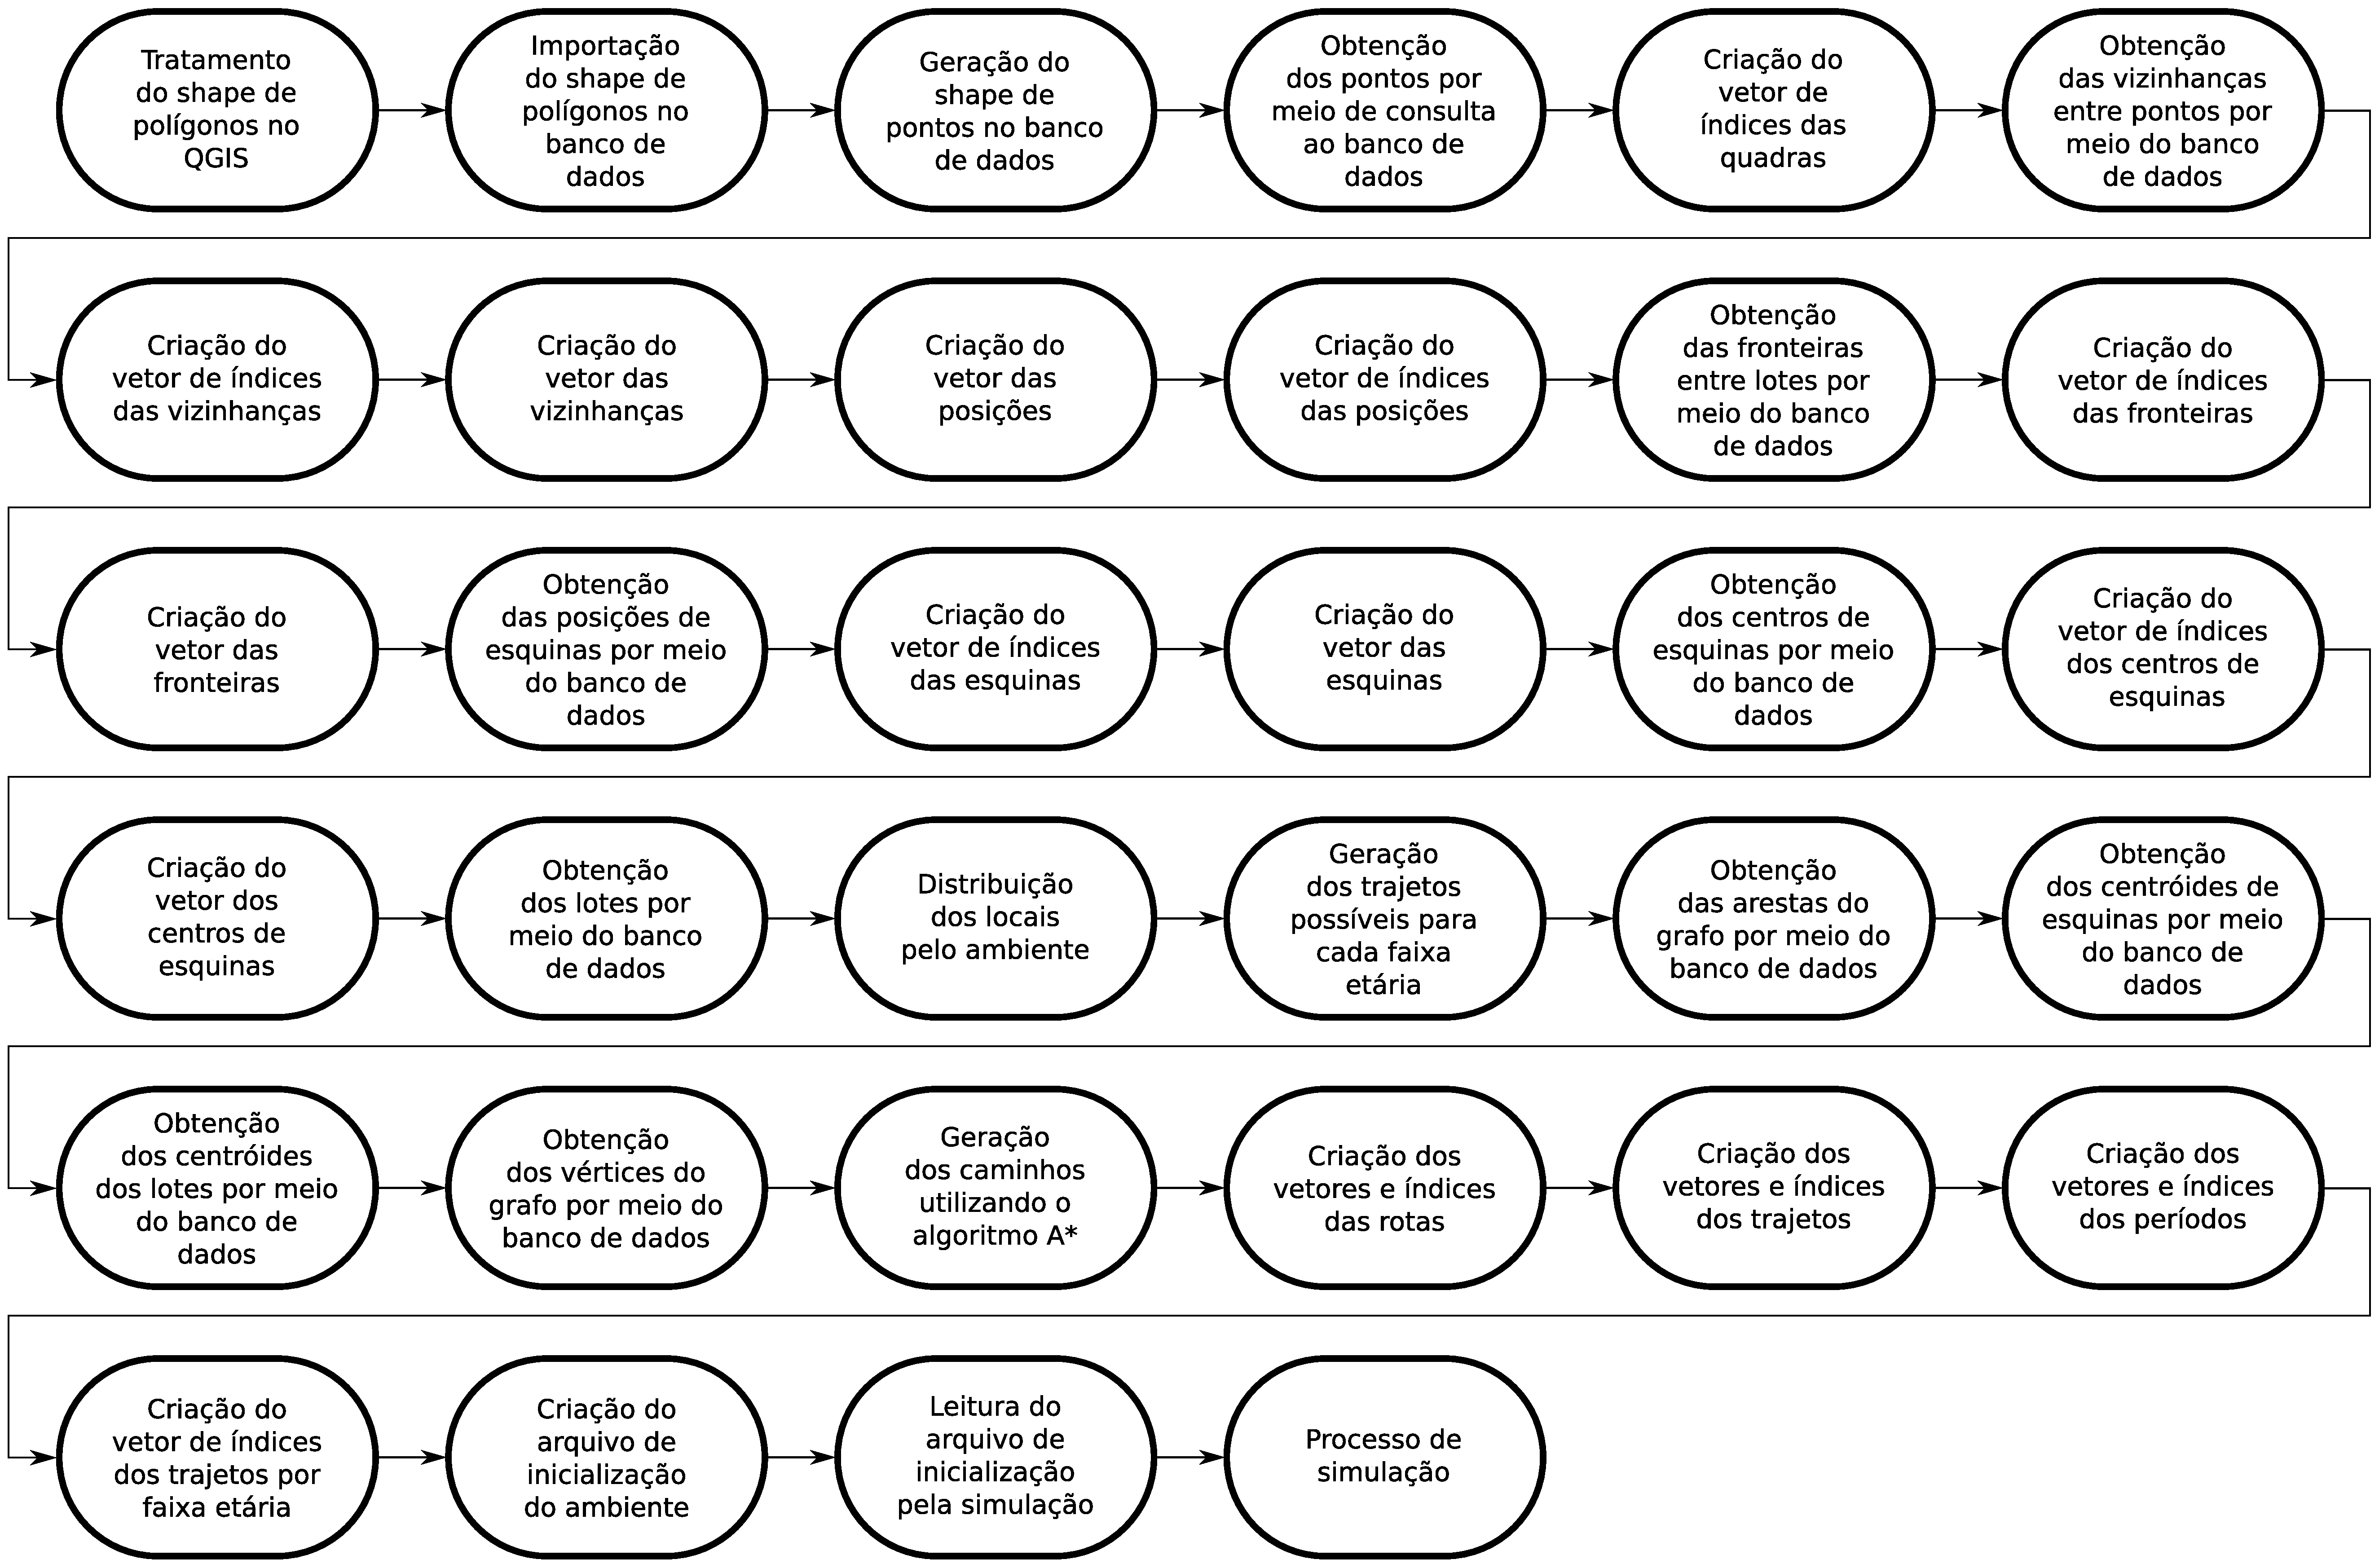
\includegraphics[width=1\textwidth]{Figuras/Simula/inicializacaoAmbiente.eps}
  \caption{Fluxograma das operações realizadas para a inicialização de um ambiente de simulação.}
  \label{fig:inicializacaoAmbiente}
\end{figure} 

\newpage

Abaixo são ilustrados os códigos fonte e algoritmos das rotinas responsáveis pela geração do arquivo de inicialização dos ambientes computacionais. Nos algoritmos os detalhes computacionais de implementação foram abstraídos para sintetizar de forma concisa os passos necessários à conclusão da rotina e transmitir de modo geral a ideia aplicada. No Código \ref{cod:mainAmb}, Algoritmo \ref{alg:mainAmb} e Figura \ref{fig:mainAmb} é apresentado o algoritmo principal que controla a geração do arquivo de inicialização de um ambiente. Este código é responsável pela execução da maioria das operações ilustradas na Figura \ref{fig:inicializacaoAmbiente}. Neste código são definidas as variáveis \textit{nCasa}, \textit{nTrabalho}, \textit{nLazer} e \textit{nEstudos}, que armazenam as quantidades de lotes que serão definidos como casa, trabalho, lazer e estudo nas rotinas de geração de trajetos. 

\subsubsection{Função Principal}

\lstinputlisting[caption=Função Principal, label=cod:mainAmb, captionpos=b, language=Java]{Codigos/Simula/Fontes/main.java}

\begin{algorithm}[H]
   \SetAlgoLined   
   \input{Codigos/Simula/Algoritmos/main.txt}
   \caption{\textsc{Função Principal à Inicialização do Ambiente.}}
   \label{alg:mainAmb}
\end{algorithm}

\begin{figure}[H]
  \centering
  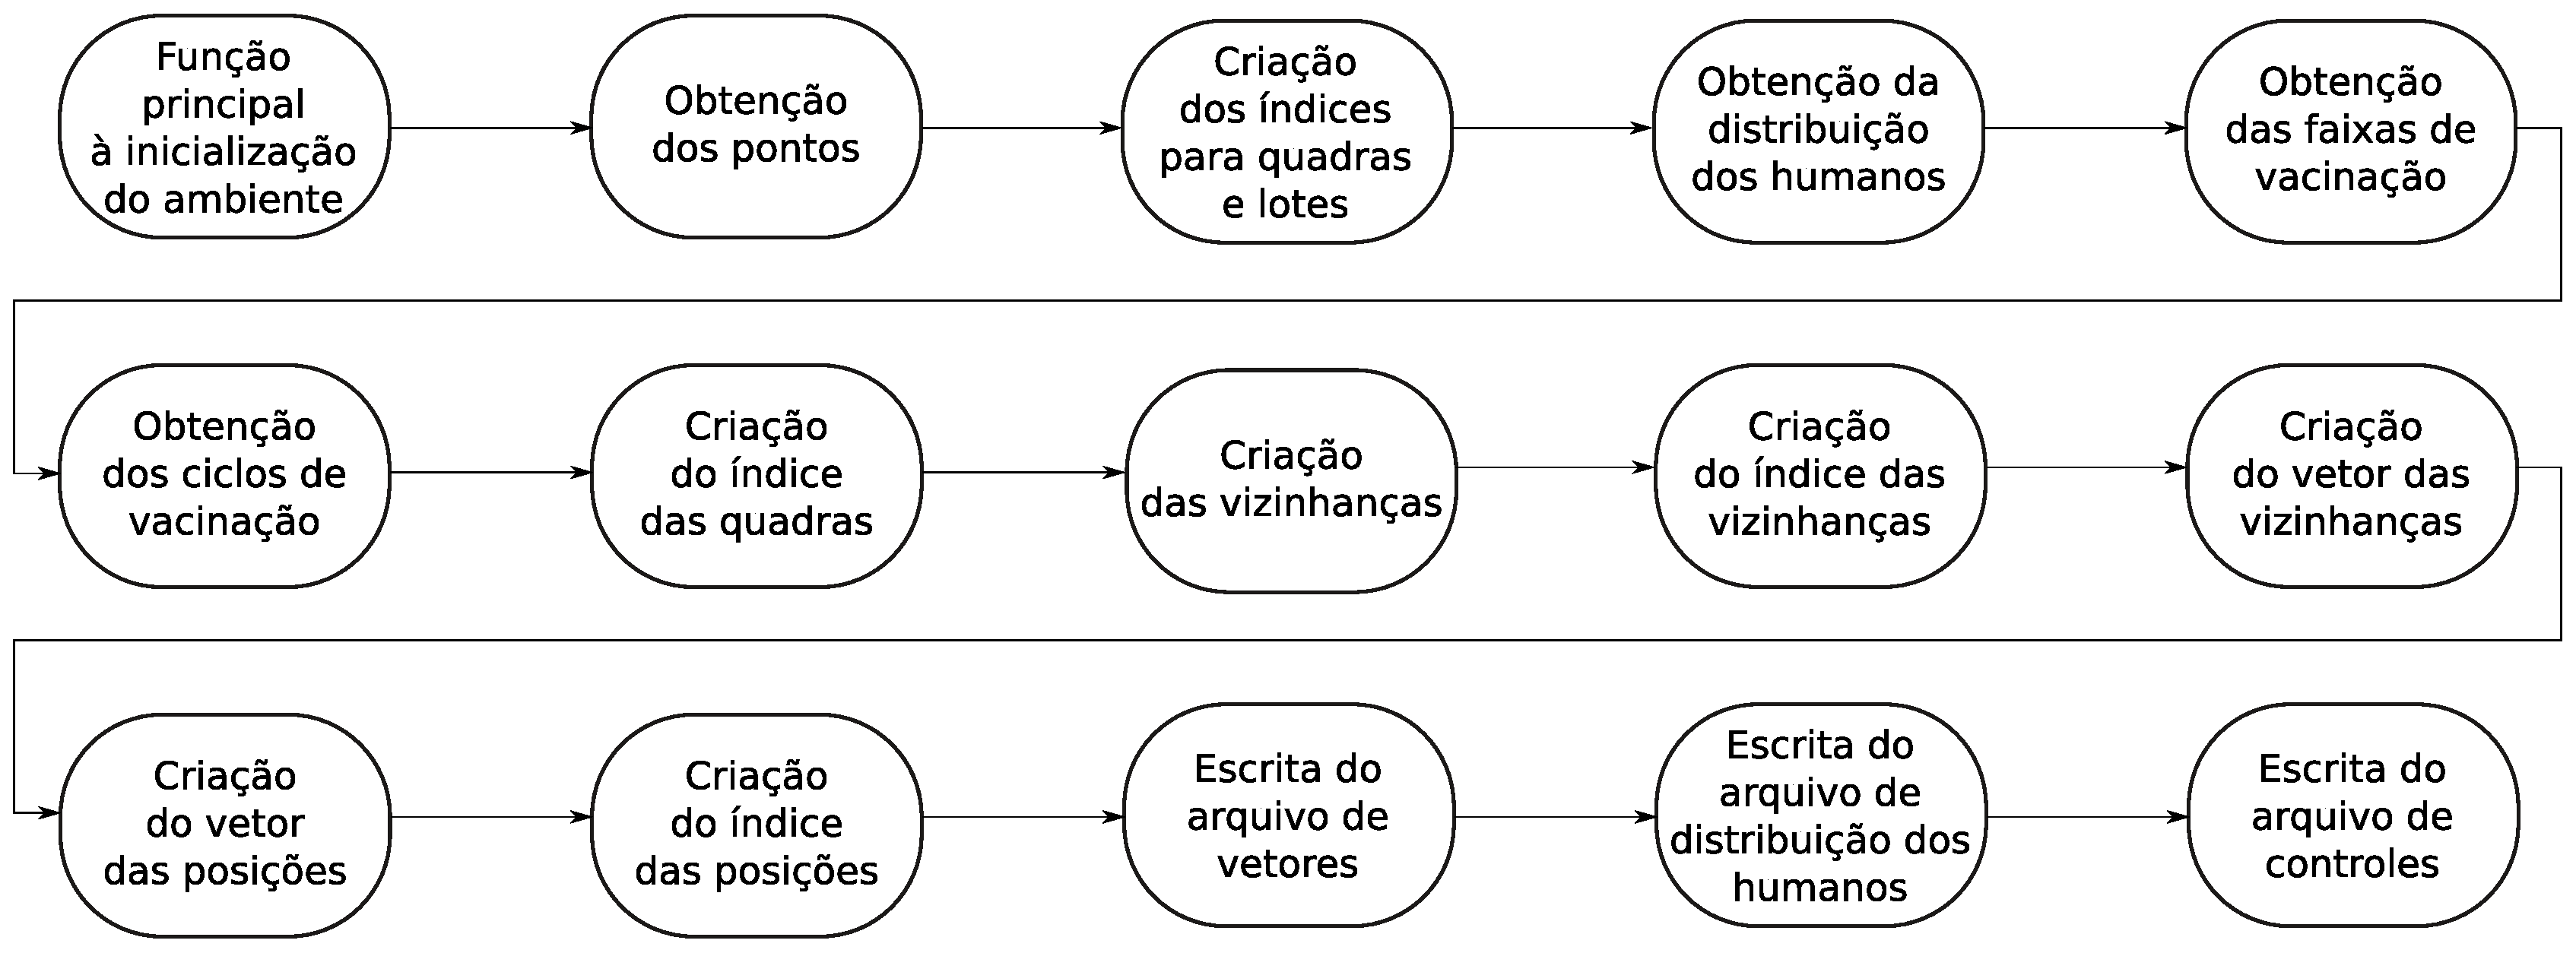
\includegraphics[width=1\textwidth]{Figuras/Simula/Fluxos/Main.eps}
  \caption{Função Principal à Inicialização do Ambiente.}
  \label{fig:mainAmb}
\end{figure} 

\newpage

\subsubsection{Função getPontosLoteseRuas}

O Código \ref{cod:getPontosLoteseRuas}, Algoritmo \ref{alg:getPontosLoteseRuas} e Figura \ref{fig:getPontosLoteseRuas} ilustram a rotina responsável pela obtenção dos pontos dos lotes e ruas. Esta rotina realiza uma consulta ao banco de dados para obter as informações armazenadas na tabela com sufixo \textit{"\_pontosloteseruas"}. A função de criação e um exemplo da tabela são ilustrados no Código \ref{cod:sql_getPontosLotesERuas} e Tabela \ref{tab:cascavel_pontosloteseruas}.

\lstinputlisting[caption=Função getPontosLoteseRuas, label=cod:getPontosLoteseRuas, captionpos=b, language=Java]{Codigos/Simula/Fontes/getPontosLoteseRuas.java}

\begin{algorithm}[H]
   \SetAlgoLined   
   \input{Codigos/Simula/Algoritmos/getPontosLoteseRuas.txt}
   \caption{\textsc{Função getPontosLoteseRuas.}}
   \label{alg:getPontosLoteseRuas}
\end{algorithm}

\begin{figure}[H]
  \centering
  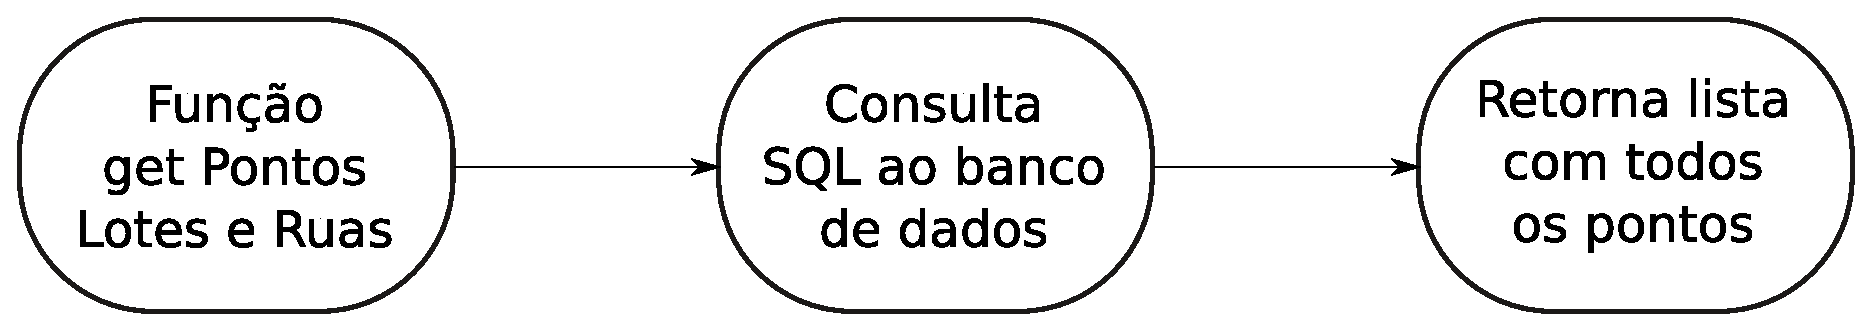
\includegraphics[width=0.7\textwidth]{Figuras/Simula/Fluxos/getPontosLoteseRuas.eps}
  \caption{Função getPontosLoteseRuas.}
  \label{fig:getPontosLoteseRuas}
\end{figure} 

\newpage

\subsubsection{Função criarIndexQuadraseLotes}

O Código \ref{cod:criarIndexQuadraseLotes}, Algoritmo \ref{alg:criarIndexQuadraseLotes} e Figura \ref{fig:criarIndexQuadraseLotes}, ilustram a rotina responsável pela criação de estruturas auxiliares ao processo que geração do arquivo de inicialização do ambiente. Estas estruturas mapeiam as cadeias de caracteres dos identificadores de quadra e lotes em números inteiros, que são utilizados posteriormente pela simulação. Deste modo, durante a simulação as quadras e lotes são identificadas por números inteiros e não por seus identificadores originais. 

\lstinputlisting[caption=Função criarIndexQuadraseLotes, label=cod:criarIndexQuadraseLotes, captionpos=b, language=Java]{Codigos/Simula/Fontes/criarIndexQuadraseLotes.java}

\begin{algorithm}[H]
   \SetAlgoLined   
   \input{Codigos/Simula/Algoritmos/criarIndexQuadraseLotes.txt}
   \caption{\textsc{Função criarIndexQuadraseLotes.}}
   \label{alg:criarIndexQuadraseLotes}
\end{algorithm}

\begin{figure}[H]
  \centering
  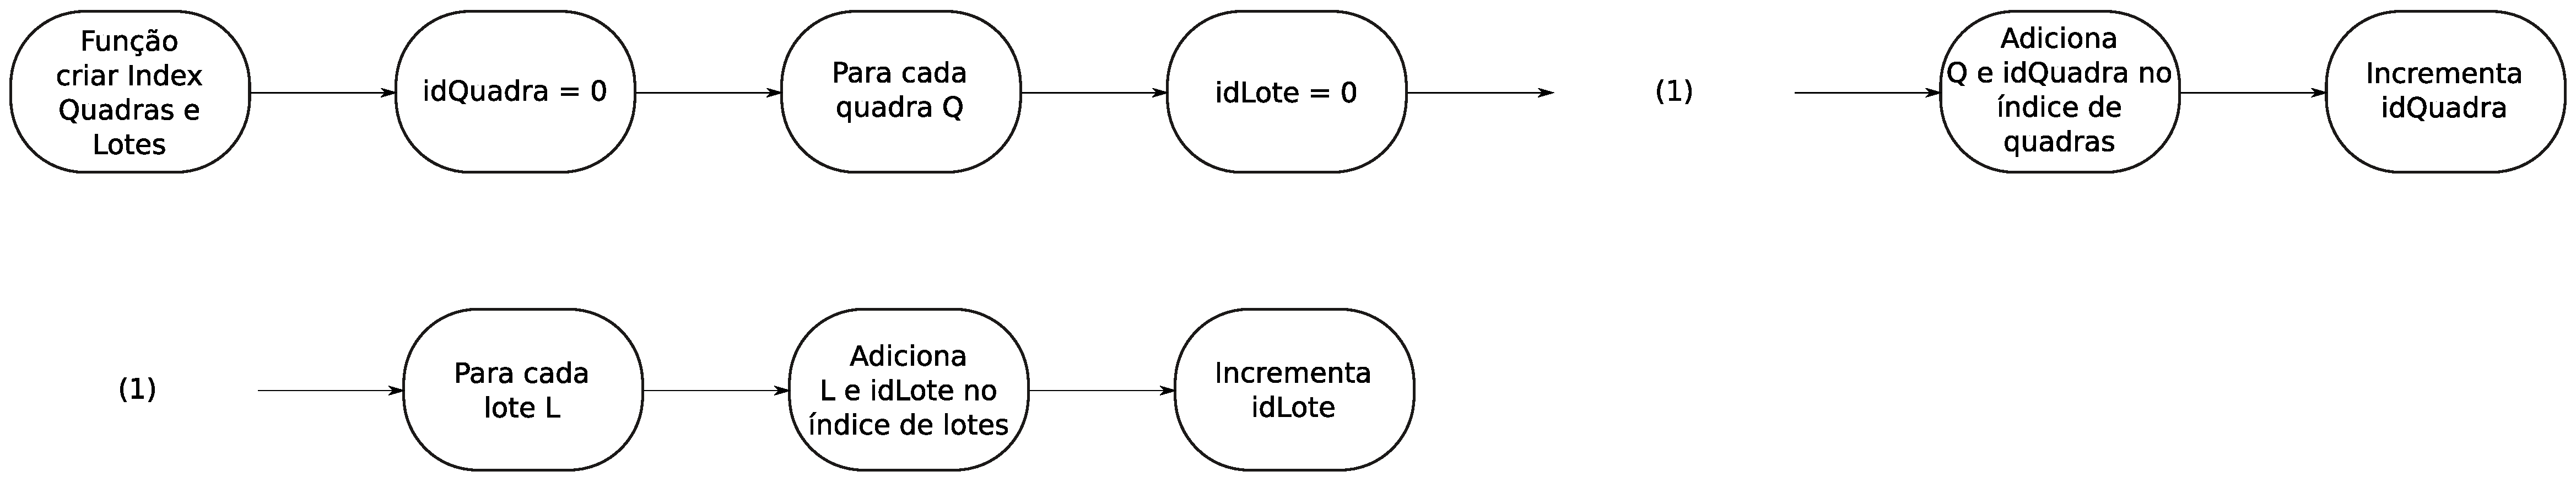
\includegraphics[width=1\textwidth]{Figuras/Simula/Fluxos/criarIndexQuadraseLotes.eps}
  \caption{Função criarIndexQuadraseLotes.}
  \label{fig:criarIndexQuadraseLotes}
\end{figure} 

\newpage

\subsubsection{Função gerarIndexQuadras}

O Código \ref{cod:gerarIndexQuadras}, Algoritmo \ref{alg:gerarIndexQuadras} e Figura \ref{fig:gerarIndexQuadras} ilustram a rotina responsável pela criação do vetor de índices para as quadras. Este índice é empregado à redução do tempo de execução das simulações por diminuir significativamente os espaços de busca em operações relacionadas ao ambiente computacional. Em posse do identificador numérico de uma quadra, esta estrutura de índice viabiliza o acesso aos lotes e vértices que pertencem à esta quadra em tempo constante. 

\lstinputlisting[caption=Função gerarIndexQuadras, label=cod:gerarIndexQuadras, captionpos=b, language=Java]{Codigos/Simula/Fontes/gerarIndexQuadras.java}

\begin{algorithm}[H]
   \SetAlgoLined   
   \input{Codigos/Simula/Algoritmos/gerarIndexQuadras.txt}
   \caption{\textsc{Função gerarIndexQuadras.}}
   \label{alg:gerarIndexQuadras}
\end{algorithm}

\begin{figure}[H]
  \centering
  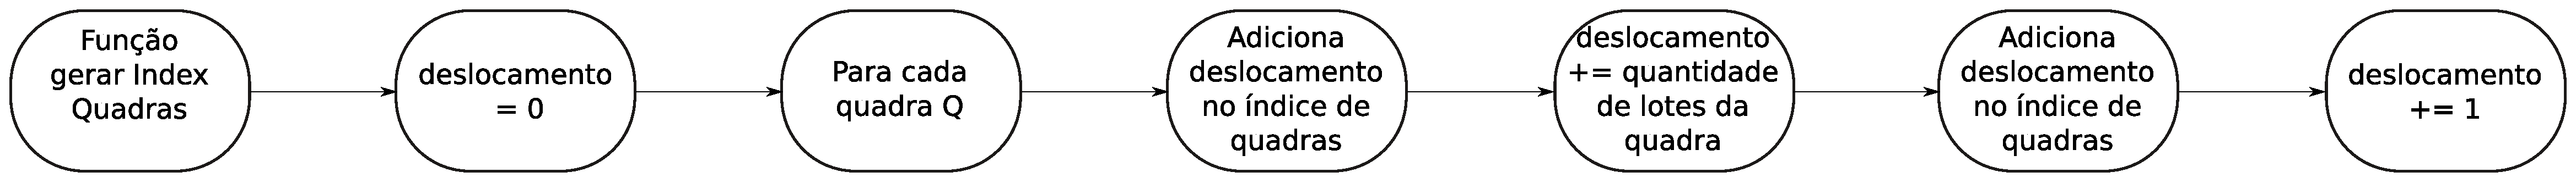
\includegraphics[width=1\textwidth]{Figuras/Simula/Fluxos/gerarIndexQuadras.eps}
  \caption{Função gerarIndexQuadras.}
  \label{fig:gerarIndexQuadras}
\end{figure} 

\newpage

\subsubsection{Função gerarVizinhancas}

O Código \ref{cod:gerarVizinhancas}, Algoritmo \ref{alg:gerarVizinhancas} e Figura \ref{fig:gerarVizinhancas} ilustram a rotina responsável pelo tratamento das vizinhanças de Moore entre os vértices obtida pela rotina apresentada no Código \ref{cod:getVizinhancasMoorePontos} e Algoritmo \ref{alg:getVizinhancasMoorePontos}. É realizada uma operação de ordenação sobre o conjunto final de dados com o objetivo de organizar todas as vizinhanças em posições contíguas na estrutura. Deste modo, índices podem ser gerados e empregados à redução dos espaços de busca pela vizinhança de um vértice específico. 

\lstinputlisting[caption=Função gerarVizinhancas, label=cod:gerarVizinhancas, captionpos=b, language=Java]{Codigos/Simula/Fontes/gerarVizinhancas.java}

\begin{algorithm}[H]
   \SetAlgoLined   
   \input{Codigos/Simula/Algoritmos/gerarVizinhancas.txt}
   \caption{\textsc{Função gerarVizinhancas.}}
   \label{alg:gerarVizinhancas}
\end{algorithm}

\begin{figure}[H]
  \centering
  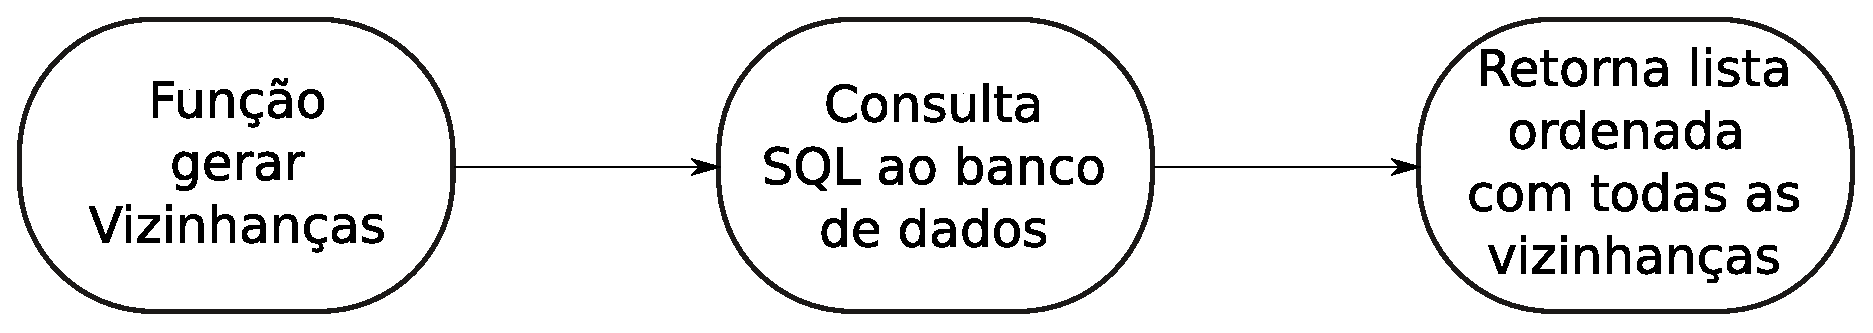
\includegraphics[width=0.7\textwidth]{Figuras/Simula/Fluxos/gerarVizinhancas.eps}
  \caption{Função gerarVizinhancas.}
  \label{fig:gerarVizinhancas}
\end{figure} 

\newpage

\subsubsection{Função getVizinhancasEntrePoligonos}

O Código \ref{cod:getVizinhancasEntrePoligonos}, Algoritmo \ref{alg:getVizinhancasEntrePoligonos} e Figura \ref{fig:getVizinhancasEntrePoligonos} ilustram a rotina responsável pela obtenção das vizinhanças entre polígonos. Esta rotina realiza uma consulta ao banco de dados para obter as informações armazenadas na tabela com sufixo \textit{"\_vizinhancasentrepoligonos"}. A função de criação e um exemplo da tabela são ilustrados no Código \ref{cod:sql_getVizinhancasEntrePoligonos} e Tabela \ref{tab:cascavel_vizinhancasentrepoligonos}. 

\lstinputlisting[caption=Função getVizinhancasEntrePoligonos, label=cod:getVizinhancasEntrePoligonos, captionpos=b, language=Java]{Codigos/Simula/Fontes/getVizinhancasEntrePoligonos.java}

\begin{algorithm}[H]
   \SetAlgoLined   
   \input{Codigos/Simula/Algoritmos/getVizinhancasEntrePoligonos.txt}
   \caption{\textsc{Função getVizinhancasEntrePoligonos.}}
   \label{alg:getVizinhancasEntrePoligonos}
\end{algorithm}

\begin{figure}[H]
  \centering
  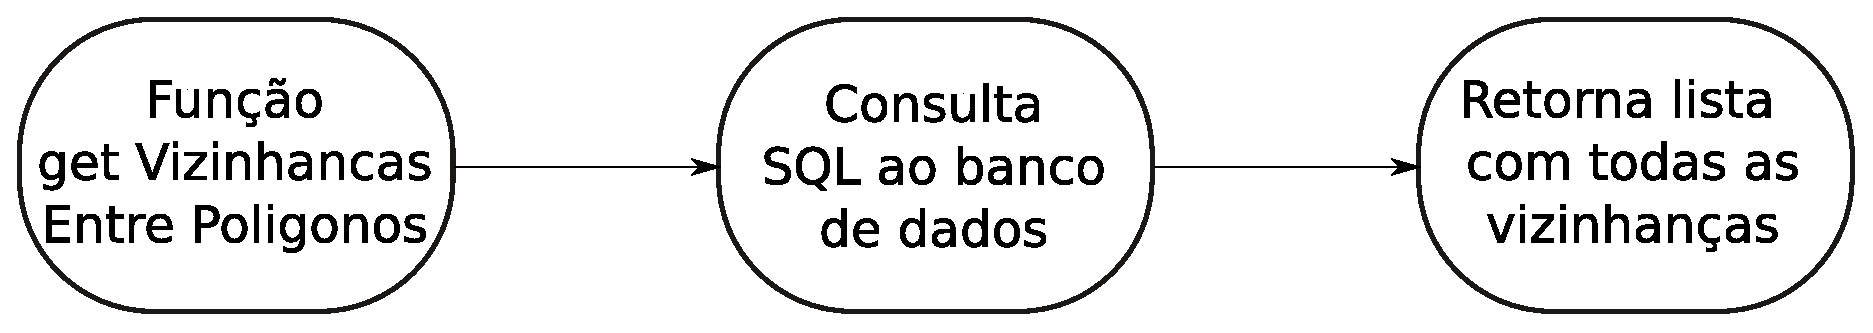
\includegraphics[width=0.7\textwidth]{Figuras/Simula/Fluxos/getVizinhancasEntrePoligonos.eps}
  \caption{Função getVizinhancasEntrePoligonos.}
  \label{fig:getVizinhancasEntrePoligonos}
\end{figure} 

\newpage

\subsubsection{Função getVizinhancasMoorePontos}

O Código \ref{cod:getVizinhancasMoorePontos}, Algoritmo \ref{alg:getVizinhancasMoorePontos} e Figura \ref{fig:getVizinhancasMoorePontos} ilustram a rotina responsável pela obtenção das vizinhanças de Moore entre os vértices. Esta rotina realiza uma consulta ao banco de dados para obter as informações armazenadas na tabela com sufixo \textit{"\_vizinhancasmoorepontos"}. A função de criação e um exemplo da tabela são ilustrados no Código \ref{cod:sql_getVizinhancasMoorePontos} e Tabela \ref{tab:cascavel_vizinhancasmoorepontos}.  

\lstinputlisting[caption=Função getVizinhancasMoorePontos, label=cod:getVizinhancasMoorePontos, captionpos=b, language=Java]{Codigos/Simula/Fontes/getVizinhancasMoorePontos.java}

\begin{algorithm}[H]
   \SetAlgoLined   
   \input{Codigos/Simula/Algoritmos/getVizinhancasMoorePontos.txt}
   \caption{\textsc{Função getVizinhancasMoorePontos.}}
   \label{alg:getVizinhancasMoorePontos}
\end{algorithm}

\begin{figure}[H]
  \centering
  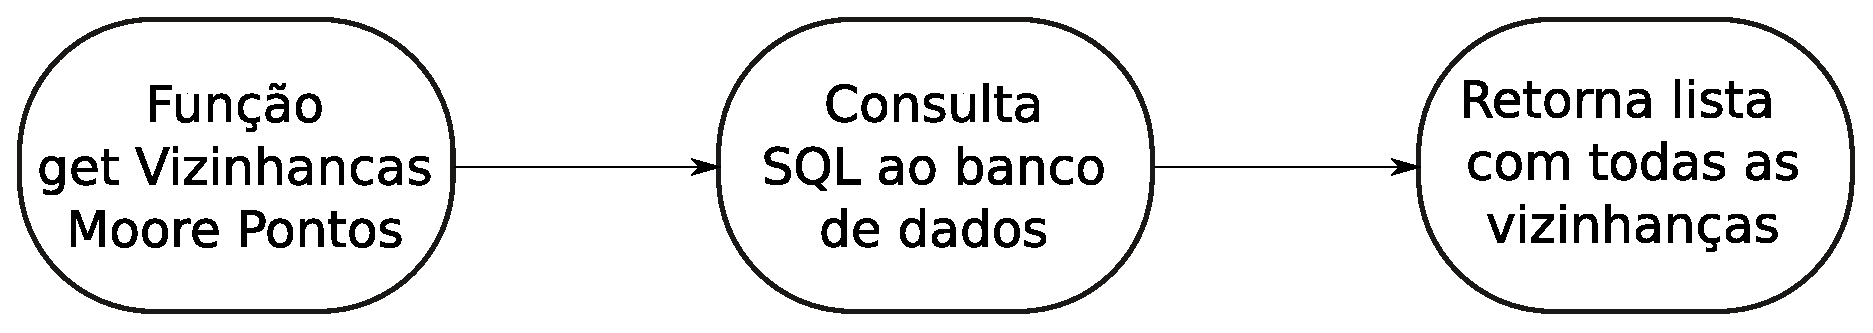
\includegraphics[width=0.7\textwidth]{Figuras/Simula/Fluxos/getVizinhancasMoorePontos.eps}
  \caption{Função getVizinhancasMoorePontos.}
  \label{fig:getVizinhancasMoorePontos}
\end{figure} 

\newpage

\subsubsection{Função gerarIndexVizinhancas}

O Código \ref{cod:gerarIndexVizinhancas}, Algoritmo \ref{alg:gerarIndexVizinhancas} e Figura \ref{fig:gerarIndexVizinhancas} ilustram a rotina responsável pela geração dos índices para as estruturas de vizinhanças entre vértices. Este índice é gerado à nível de lote e utilizado juntamente com o índice de quadras, viabilizando a recuperação rápida das vizinhanças de Moore entre vértices se conhecidos os identificadores numéricos da quadra e do lote. 

\lstinputlisting[caption=Função gerarIndexVizinhancas, label=cod:gerarIndexVizinhancas, captionpos=b, language=Java]{Codigos/Simula/Fontes/gerarIndexVizinhancas.java}

\begin{algorithm}[H]
   \SetAlgoLined   
   \input{Codigos/Simula/Algoritmos/gerarIndexVizinhancas.txt}
   \caption{\textsc{Função gerarIndexVizinhancas.}}
   \label{alg:gerarIndexVizinhancas}
\end{algorithm}

\begin{figure}[H]
  \centering
  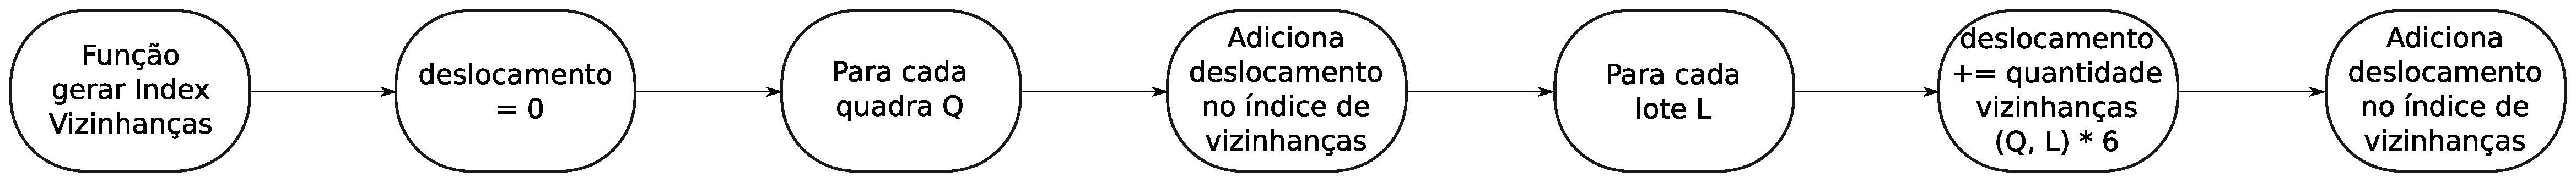
\includegraphics[width=1\textwidth]{Figuras/Simula/Fluxos/gerarIndexVizinhancas.eps}
  \caption{Função gerarIndexVizinhancas.}
  \label{fig:gerarIndexVizinhancas}
\end{figure} 

\newpage

\subsubsection{Função gerarVetorVizinhancas}

O Código \ref{cod:gerarVetorVizinhancas}, Algoritmo \ref{alg:gerarVetorVizinhancas} e Figura \ref{fig:gerarVetorVizinhancas} ilustram a rotina responsável pela geração do vetor que armazena todas as vizinhanças entre vértices. Nesta rotina as informações pertencentes às vizinhanças, armazenadas em classes, são dispostas e organizadas em uma estrutura linear, que é mapeada posteriormente à um vetor de tipo homogêneo, facilitando à cópia de dados à GPU.

\lstinputlisting[caption=Função gerarVetorVizinhancas, label=cod:gerarVetorVizinhancas, captionpos=b, language=Java]{Codigos/Simula/Fontes/gerarVetorVizinhancas.java}

\begin{algorithm}[H]
   \SetAlgoLined   
   \input{Codigos/Simula/Algoritmos/gerarVetorVizinhancas.txt}
   \caption{\textsc{Função gerarVetorVizinhancas.}}
   \label{alg:gerarVetorVizinhancas}
\end{algorithm}

\begin{figure}[H]
  \centering
  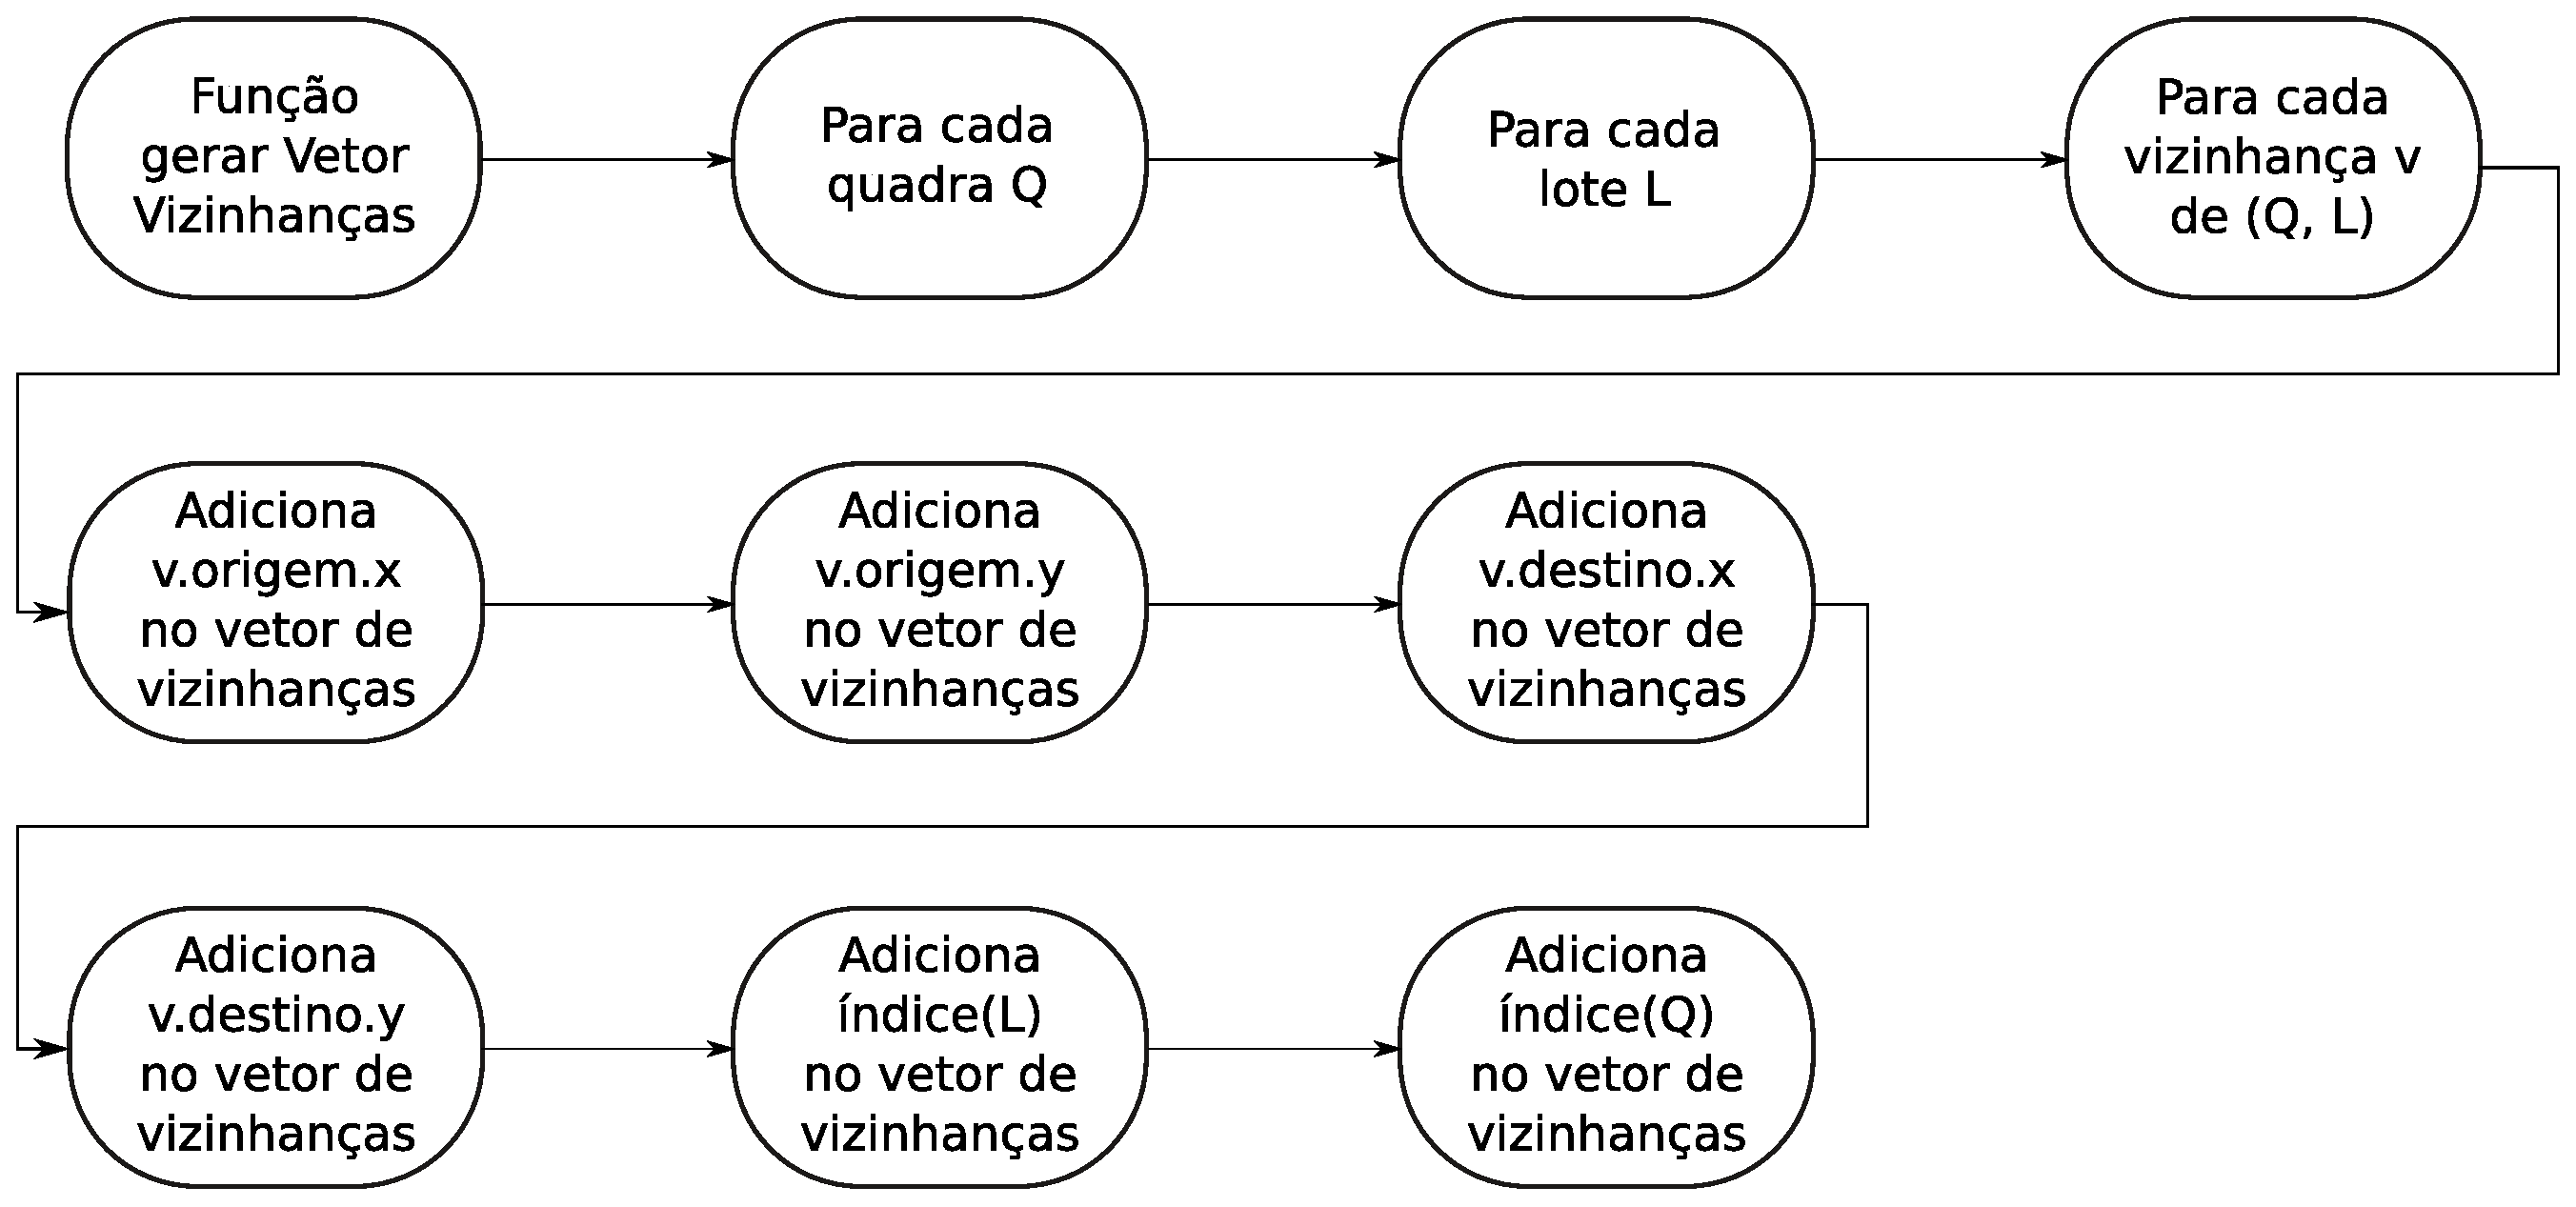
\includegraphics[width=0.8\textwidth]{Figuras/Simula/Fluxos/gerarVetorVizinhancas.eps}
  \caption{Função gerarVetorVizinhancas.}
  \label{fig:gerarVetorVizinhancas}
\end{figure} 

\newpage

\subsubsection{Função gerarVetorPosicoes}

O Código \ref{cod:gerarVetorPosicoes}, Algoritmo \ref{alg:gerarVetorPosicoes} e Figura \ref{fig:gerarVetorPosicoes} ilustram a rotina responsável pela geração do vetor que armazena todos os vértices. Nesta rotina os vértices armazenados em classes são dispostos e organizados em uma estrutura linear, que é mapeada posteriormente à um vetor de tipo homogêneo, facilitando à cópia de dados à GPU.

\lstinputlisting[caption=Função gerarVetorPosicoes, label=cod:gerarVetorPosicoes, captionpos=b, language=Java]{Codigos/Simula/Fontes/gerarVetorPosicoes.java}

\begin{algorithm}[H]
   \SetAlgoLined   
   \input{Codigos/Simula/Algoritmos/gerarVetorPosicoes.txt}
   \caption{\textsc{Função gerarVetorPosicoes.}}
   \label{alg:gerarVetorPosicoes}
\end{algorithm}

\begin{figure}[H]
  \centering
  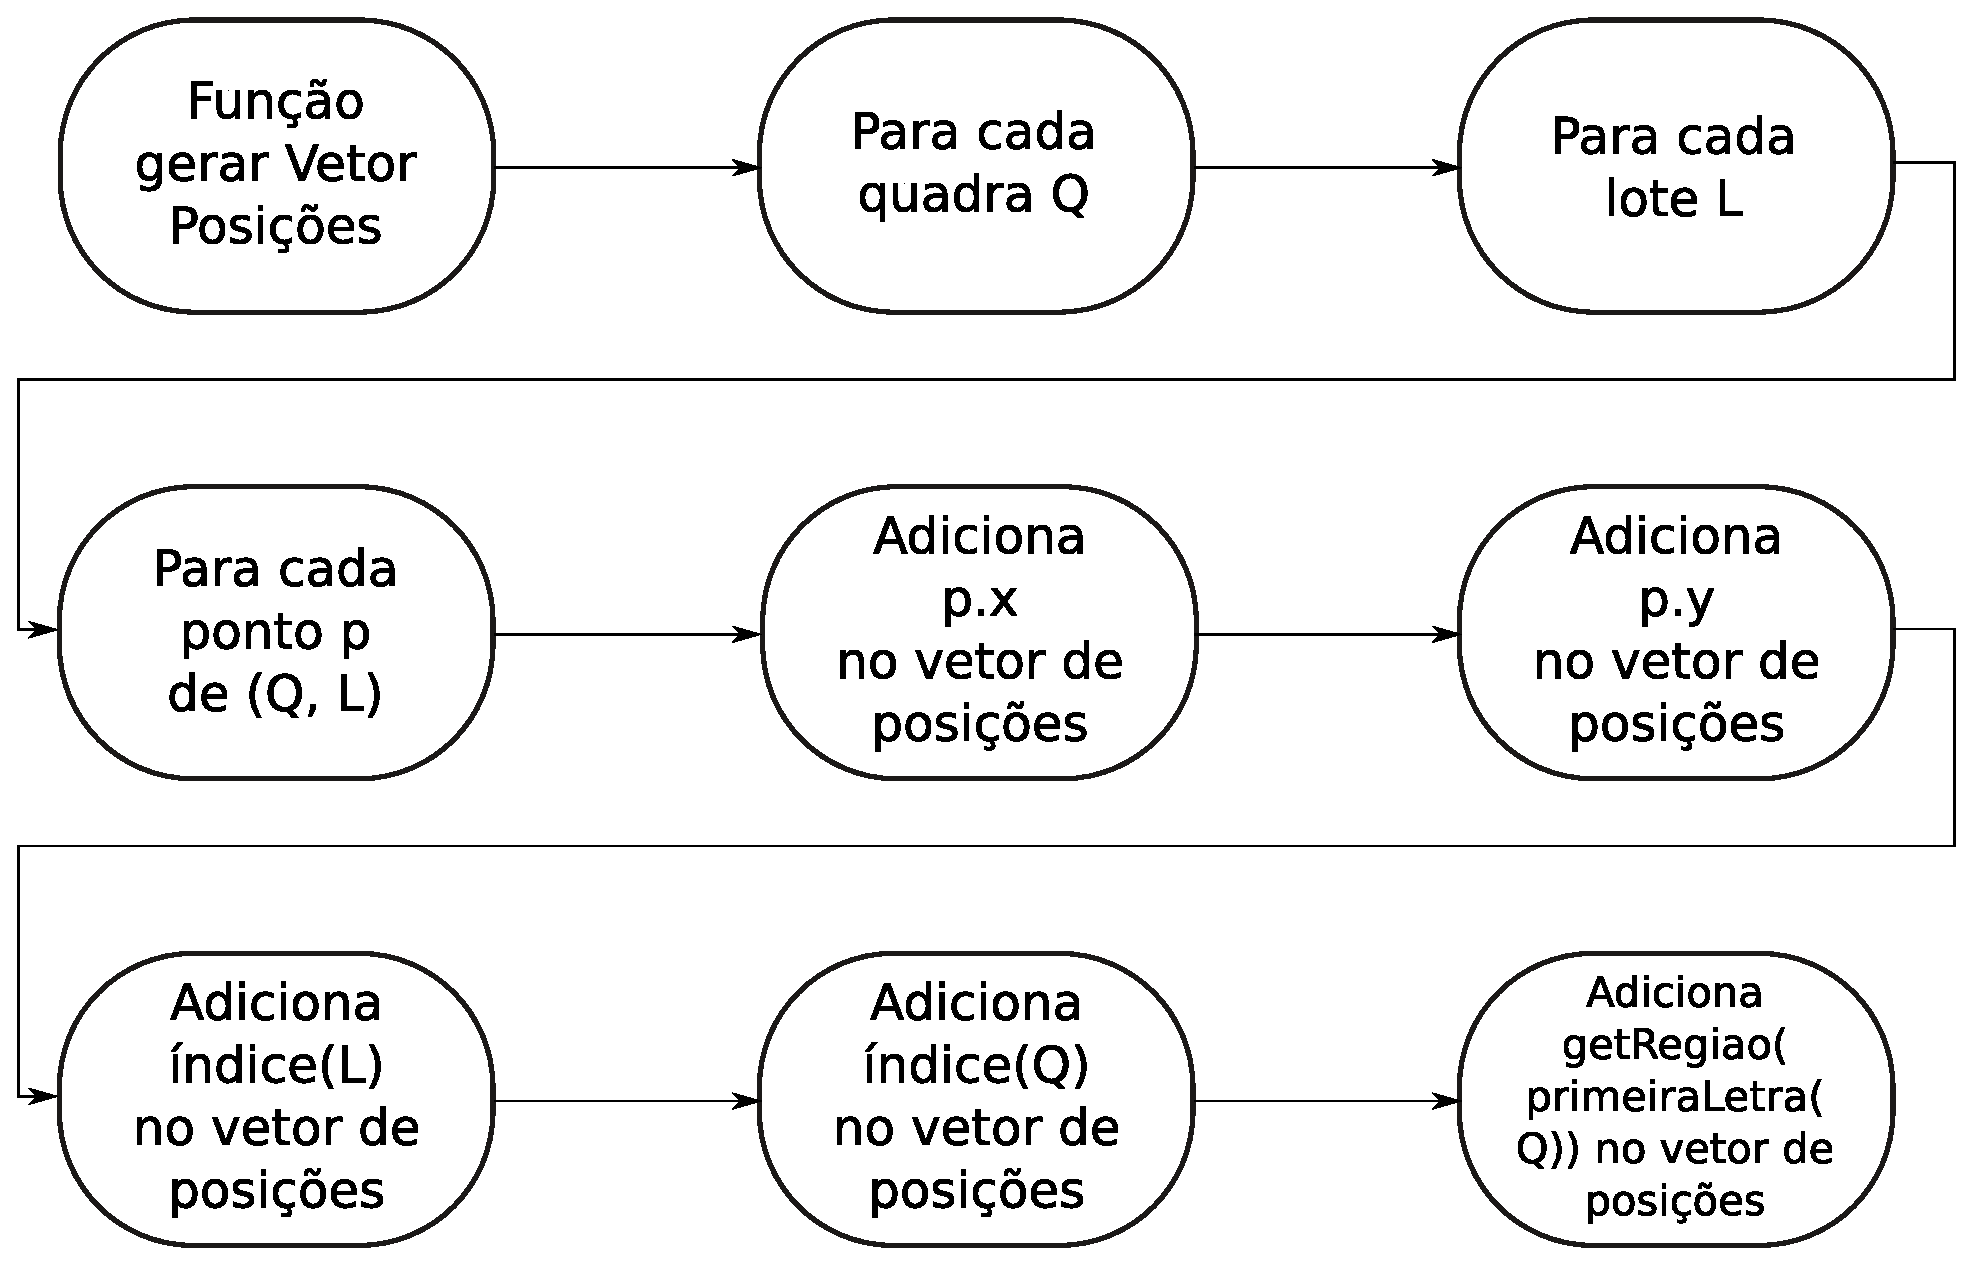
\includegraphics[width=0.6\textwidth]{Figuras/Simula/Fluxos/gerarVetorPosicoes.eps}
  \caption{Função gerarVetorPosicoes.}
  \label{fig:gerarVetorPosicoes}
\end{figure} 

\newpage

\subsubsection{Função gerarIndexPosicoes}

O Código \ref{cod:gerarIndexPosicoes}, Algoritmo \ref{alg:gerarIndexPosicoes} e Figura \ref{fig:gerarIndexPosicoes} ilustram a rotina responsável pela geração dos índices aos vértices do ambiente. Este índice é gerado à nível de lote e utilizado juntamente com o índice de quadras, viabilizando a recuperação rápida de todos vértices pertencentes à um lote de uma quadra. Os identificadores numéricos da quadra e do lote são utilizados como índices. 

\lstinputlisting[caption=Função gerarIndexPosicoes, label=cod:gerarIndexPosicoes, captionpos=b, language=Java]{Codigos/Simula/Fontes/gerarIndexPosicoes.java}

\begin{algorithm}[H]
   \SetAlgoLined   
   \input{Codigos/Simula/Algoritmos/gerarIndexPosicoes.txt}
   \caption{\textsc{Função gerarIndexPosicoes.}}
   \label{alg:gerarIndexPosicoes}
\end{algorithm}

\begin{figure}[H]
  \centering
  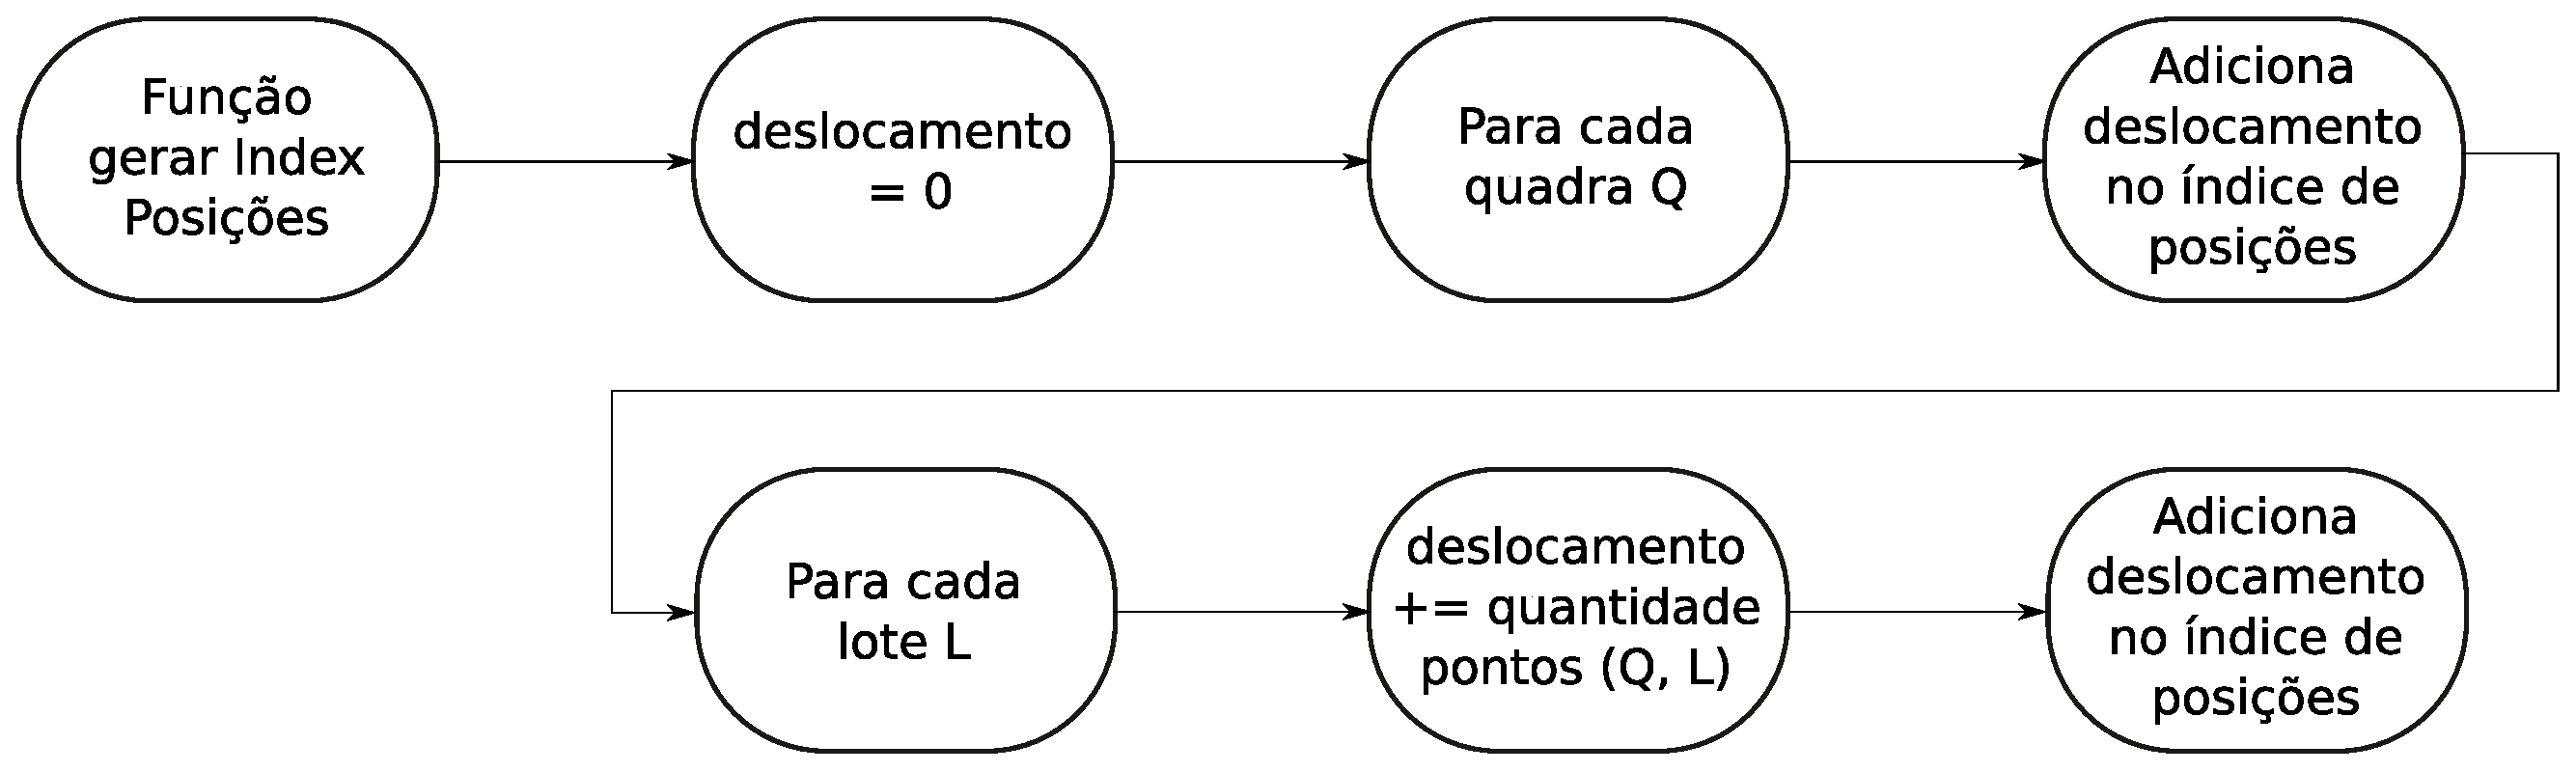
\includegraphics[width=0.8\textwidth]{Figuras/Simula/Fluxos/gerarIndexPosicoes.eps}
  \caption{Função gerarIndexPosicoes.}
  \label{fig:gerarIndexPosicoes}
\end{figure} 

\newpage

\subsubsection{Função gerarFronteiras}

O Código \ref{cod:gerarFronteiras}, Algoritmo \ref{alg:gerarFronteiras} e Figura \ref{fig:gerarFronteiras} ilustram a rotina responsável pela geração da lista de vizinhanças que pertencem à uma fronteira. As vizinhanças de fronteiras são utilizadas nos algoritmos de movimentação dos agentes. Se os vértices de origem e destino de uma vizinhança pertencem, respectivamente, à um lote e à uma rua, então ela é considerada de fronteira. Efetivamente, a rotina realiza uma operação de filtragem na lista que armazena todas as vizinhanças. 

\lstinputlisting[caption=Função gerarFronteiras, label=cod:gerarFronteiras, captionpos=b, language=Java]{Codigos/Simula/Fontes/gerarFronteiras.java}

\begin{algorithm}[H]
   \SetAlgoLined   
   \input{Codigos/Simula/Algoritmos/gerarFronteiras.txt}
   \caption{\textsc{Função gerarFronteiras.}}
   \label{alg:gerarFronteiras}
\end{algorithm}

\begin{figure}[H]
  \centering
  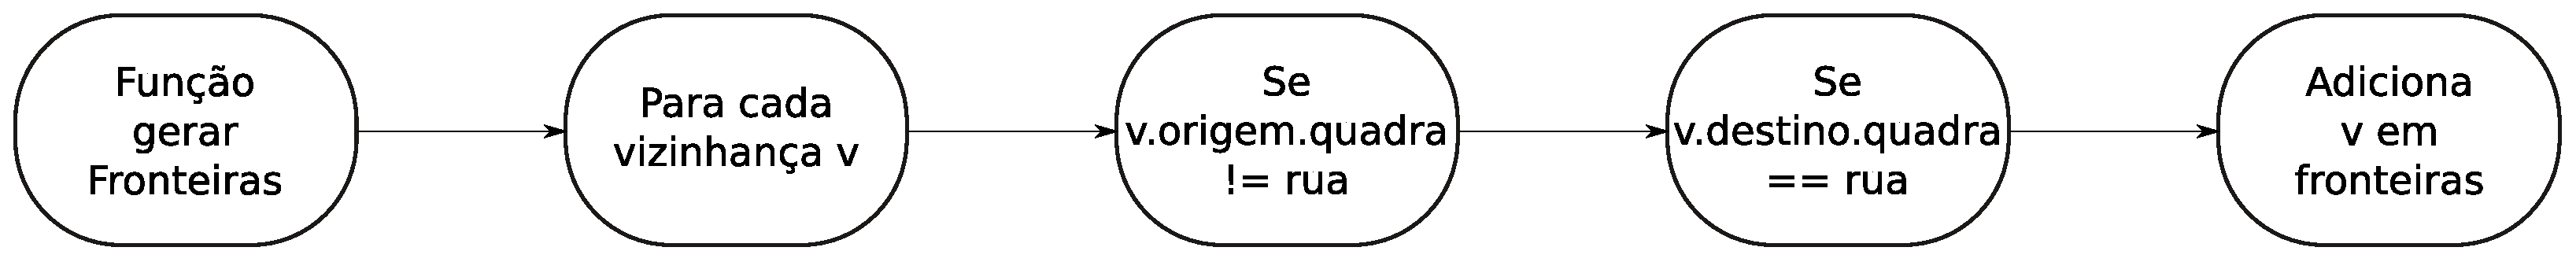
\includegraphics[width=1\textwidth]{Figuras/Simula/Fluxos/gerarFronteiras.eps}
  \caption{Função gerarFronteiras.}
  \label{fig:gerarFronteiras}
\end{figure} 

\newpage

\subsubsection{Função gerarIndexFronteiras}

O Código \ref{cod:gerarIndexFronteiras}, Algoritmo \ref{alg:gerarIndexFronteiras} e Figura \ref{fig:gerarIndexFronteiras} ilustram a rotina responsável pela geração dos índices aos vértices de fronteira. Um vértice é considerado de fronteira se pertence à um lote e possui vizinhança com pelo menos um vértice localizado em uma rua. Este índice é gerado à nível de lote e utilizado juntamente com o índice de quadras, viabilizando a recuperação rápida de todos vértices de fronteira de um lote de uma quadra. Os identificadores numéricos da quadra e do lote são utilizados como índices. Como não são considerados vértices de fronteira aos lotes de ruas, seus índices não são calculados pela rotina. 

\lstinputlisting[caption=Função gerarIndexFronteiras, label=cod:gerarIndexFronteiras, captionpos=b, language=Java]{Codigos/Simula/Fontes/gerarIndexFronteiras.java}

\begin{algorithm}[H]
   \SetAlgoLined   
   \input{Codigos/Simula/Algoritmos/gerarIndexFronteiras.txt}
   \caption{\textsc{Função gerarIndexFronteiras.}}
   \label{alg:gerarIndexFronteiras}
\end{algorithm}

\begin{figure}[H]
  \centering
  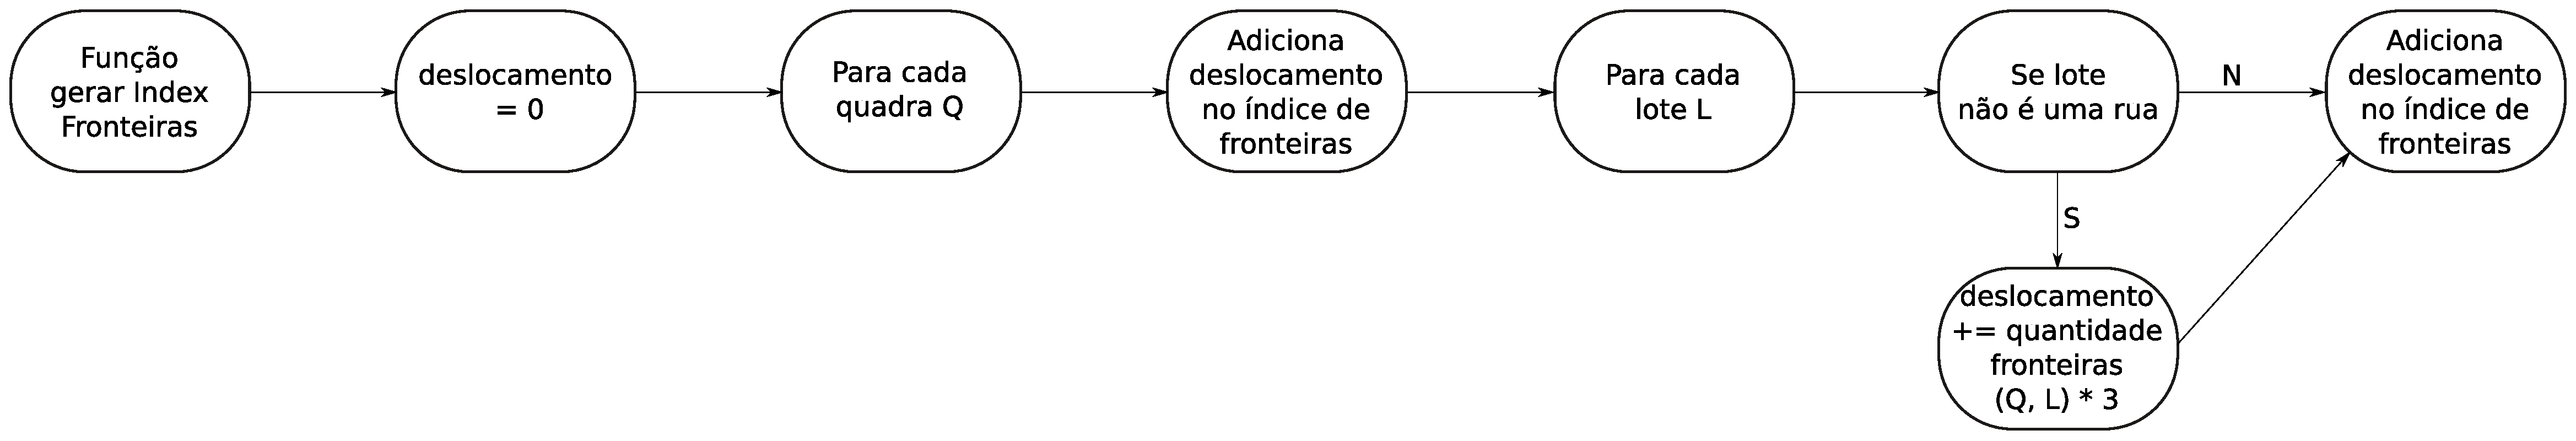
\includegraphics[width=1\textwidth]{Figuras/Simula/Fluxos/gerarIndexFronteiras.eps}
  \caption{Função gerarIndexFronteiras.}
  \label{fig:gerarIndexFronteiras}
\end{figure} 

\newpage

\subsubsection{Função gerarVetorFronteiras}

O Código \ref{cod:gerarVetorFronteiras}, Algoritmo \ref{alg:gerarVetorFronteiras} e Figura \ref{fig:gerarVetorFronteiras} ilustram a rotina responsável pela geração do vetor que armazena os vértices de fronteira. Nesta rotina os vértices armazenados em classes são dispostos e organizados em uma estrutura linear, que é mapeada posteriormente à um vetor de tipo homogêneo, facilitando à cópia de dados à GPU.

\lstinputlisting[caption=Função gerarVetorFronteiras, label=cod:gerarVetorFronteiras, captionpos=b, language=Java]{Codigos/Simula/Fontes/gerarVetorFronteiras.java}

\begin{algorithm}[H]
   \SetAlgoLined   
   \input{Codigos/Simula/Algoritmos/gerarVetorFronteiras.txt}
   \caption{\textsc{Função gerarVetorFronteiras.}}
   \label{alg:gerarVetorFronteiras}
\end{algorithm}

\begin{figure}[H]
  \centering
  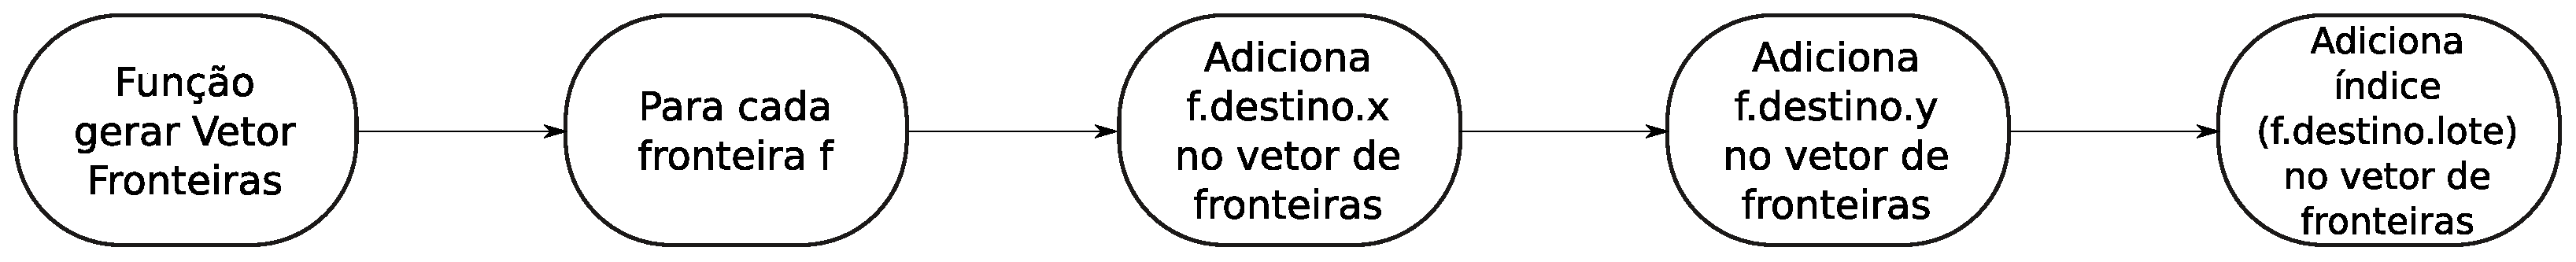
\includegraphics[width=1\textwidth]{Figuras/Simula/Fluxos/gerarVetorFronteiras.eps}
  \caption{Função gerarVetorFronteiras.}
  \label{fig:gerarVetorFronteiras}
\end{figure} 

\newpage

\subsubsection{Função getPontosEsquinas}

O Código \ref{cod:getPontosEsquinas}, Algoritmo \ref{alg:getPontosEsquinas} e Figura \ref{fig:getPontosEsquinas} ilustram a rotina responsável pela obtenção dos vértices pertencentes às esquinas. Esta rotina realiza uma consulta ao banco de dados para obter as informações armazenadas na tabela com sufixo \textit{"\_pontosesquinas"}. A função de criação e um exemplo da tabela são ilustrados no Código \ref{cod:sql_getPontosEsquinas} e Tabela \ref{tab:cascavel_pontosesquinas}.  

\lstinputlisting[caption=Função getPontosEsquinas, label=cod:getPontosEsquinas, captionpos=b, language=Java]{Codigos/Simula/Fontes/getPontosEsquinas.java}

\begin{algorithm}[H]
   \SetAlgoLined   
   \input{Codigos/Simula/Algoritmos/getPontosEsquinas.txt}
   \caption{\textsc{Função getPontosEsquinas.}}
   \label{alg:getPontosEsquinas}
\end{algorithm}

\begin{figure}[H]
  \centering
  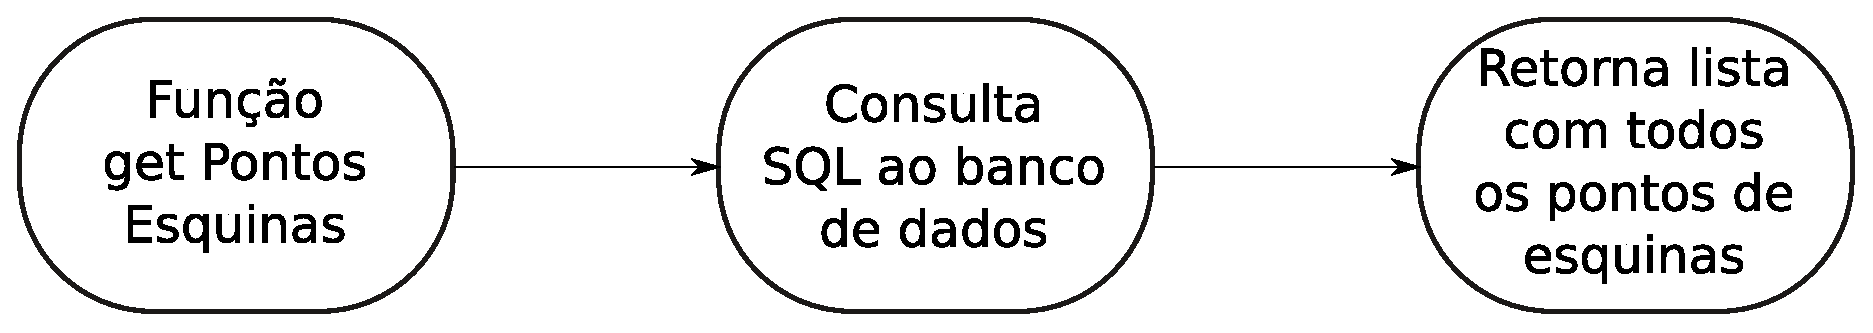
\includegraphics[width=0.7\textwidth]{Figuras/Simula/Fluxos/getPontosEsquinas.eps}
  \caption{Função getPontosEsquinas.}
  \label{fig:getPontosEsquinas}
\end{figure} 

\newpage

\subsubsection{Função gerarIndexEsquinas}

O Código \ref{cod:gerarIndexEsquinas}, Algoritmo \ref{alg:gerarIndexEsquinas} e Figura \ref{fig:gerarIndexEsquinas} ilustram a rotina responsável pela geração dos índices aos vértices de esquina. Um vértice é considerado de esquina se pertence simultaneamente à duas ruas. Este índice é gerado à nível de rua, viabilizando a recuperação rápida de todos vértices de esquina de uma rua. O identificador numérico da rua é utilizado como índice.  

\lstinputlisting[caption=Função gerarIndexEsquinas, label=cod:gerarIndexEsquinas, captionpos=b, language=Java]{Codigos/Simula/Fontes/gerarIndexEsquinas.java}

\begin{algorithm}[H]
   \SetAlgoLined   
   \input{Codigos/Simula/Algoritmos/gerarIndexEsquinas.txt}
   \caption{\textsc{Função gerarIndexEsquinas.}}
   \label{alg:gerarIndexEsquinas}
\end{algorithm}

\begin{figure}[H]
  \centering
  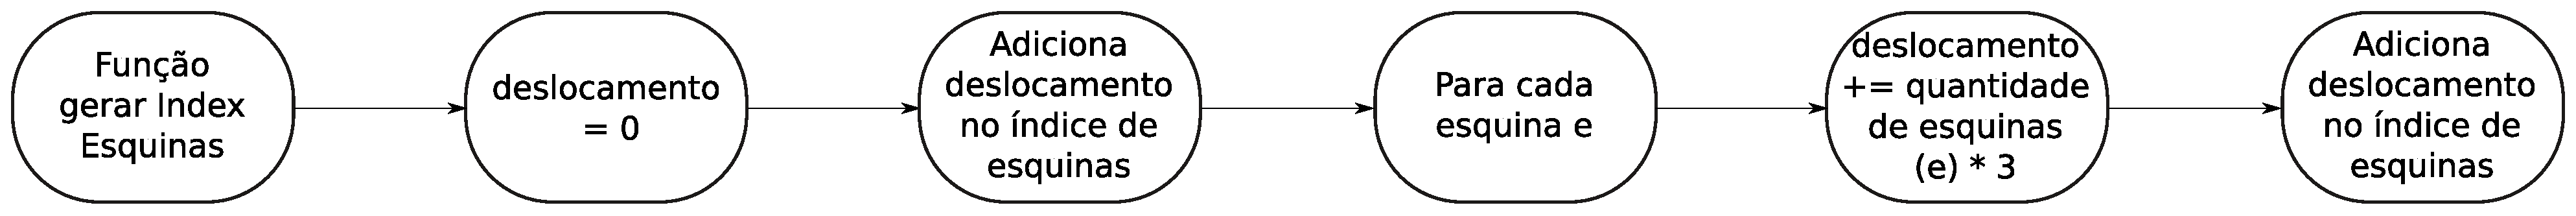
\includegraphics[width=1\textwidth]{Figuras/Simula/Fluxos/gerarIndexEsquinas.eps}
  \caption{Função gerarIndexEsquinas.}
  \label{fig:gerarIndexEsquinas}
\end{figure} 

\newpage

\subsubsection{Função gerarVetorEsquinas}

O Código \ref{cod:gerarVetorEsquinas}, Algoritmo \ref{alg:gerarVetorEsquinas} e Figura \ref{fig:gerarVetorEsquinas} ilustram a rotina responsável pela geração do vetor que armazena os vértices de esquina. Nesta rotina os vértices armazenados em classes são dispostos e organizados em uma estrutura linear, que é mapeada posteriormente à um vetor de tipo homogêneo, facilitando à cópia de dados à GPU.

\lstinputlisting[caption=Função gerarVetorEsquinas, label=cod:gerarVetorEsquinas, captionpos=b, language=Java]{Codigos/Simula/Fontes/gerarVetorEsquinas.java}

\begin{algorithm}[H]
   \SetAlgoLined   
   \input{Codigos/Simula/Algoritmos/gerarVetorEsquinas.txt}
   \caption{\textsc{Função gerarVetorEsquinas.}}
   \label{alg:gerarVetorEsquinas}
\end{algorithm}

\begin{figure}[H]
  \centering
  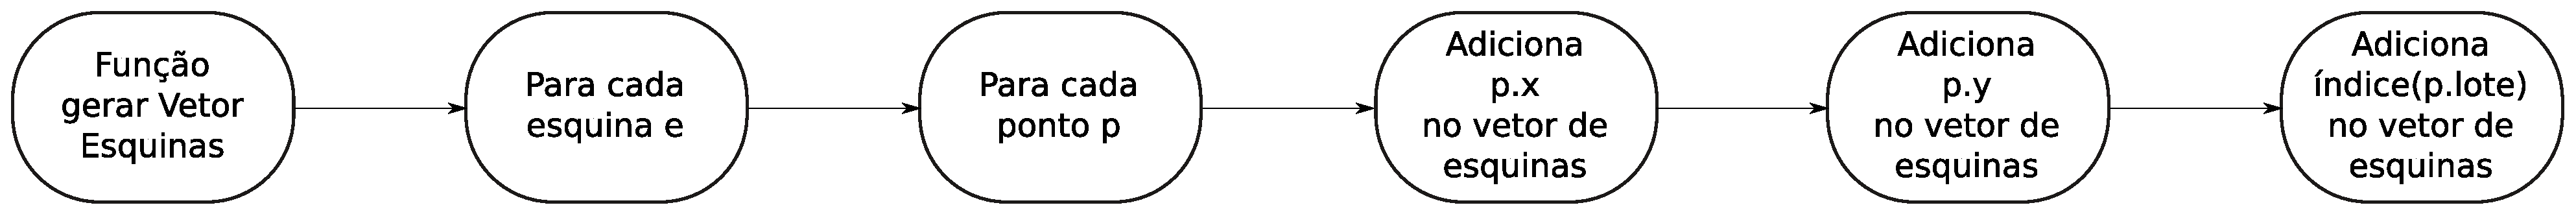
\includegraphics[width=1\textwidth]{Figuras/Simula/Fluxos/gerarVetorEsquinas.eps}
  \caption{Função gerarVetorEsquinas.}
  \label{fig:gerarVetorEsquinas}
\end{figure} 

\newpage

\subsubsection{Função gerarIndexCentrosEsquinas}

O Código \ref{cod:gerarIndexCentrosEsquinas}, Algoritmo \ref{alg:gerarIndexCentrosEsquinas} e Figura \ref{fig:gerarIndexCentrosEsquinas} ilustram a rotina responsável pela geração dos índices aos vértices centro das esquinas. Este índice é gerado à nível de rua, viabilizando a recuperação rápida de todos vértices centros de esquina de uma rua. O identificador numérico da rua é utilizado como índice.  

\lstinputlisting[caption=Função gerarIndexCentrosEsquinas, label=cod:gerarIndexCentrosEsquinas, captionpos=b, language=Java]{Codigos/Simula/Fontes/gerarIndexCentrosEsquinas.java}

\begin{algorithm}[H]
   \SetAlgoLined   
   \input{Codigos/Simula/Algoritmos/gerarIndexCentrosEsquinas.txt}
   \caption{\textsc{Função gerarIndexCentrosEsquinas.}}
   \label{alg:gerarIndexCentrosEsquinas}
\end{algorithm}

\begin{figure}[H]
  \centering
  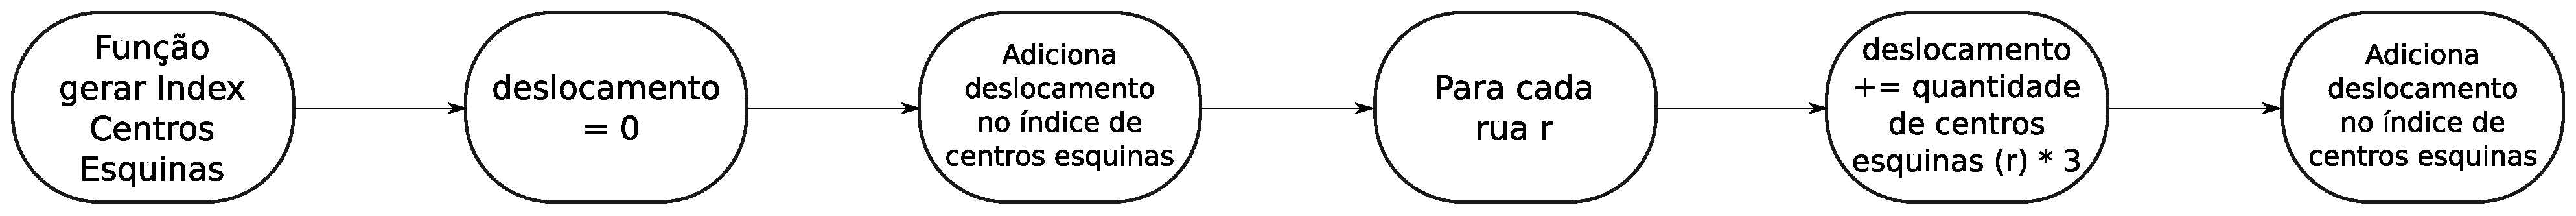
\includegraphics[width=1\textwidth]{Figuras/Simula/Fluxos/gerarIndexCentrosEsquinas.eps}
  \caption{Função gerarIndexCentrosEsquinas.}
  \label{fig:gerarIndexCentrosEsquinas}
\end{figure} 

\newpage

\subsubsection{Função gerarVetorCentrosEsquinas}

O Código \ref{cod:gerarVetorCentrosEsquinas}, Algoritmo \ref{alg:gerarVetorCentrosEsquinas} e Figura \ref{fig:gerarVetorCentrosEsquinas} ilustram a rotina responsável pela geração do vetor que armazena os vértices centro das esquinas. Nesta rotina os vértices armazenados em classes são dispostos e organizados em uma estrutura linear, que é mapeada posteriormente à um vetor de tipo homogêneo, facilitando à cópia de dados à GPU. Os vértices centro das esquinas são utilizados durante a movimentação dos agentes. 

\lstinputlisting[caption=Função gerarVetorCentrosEsquinas, label=cod:gerarVetorCentrosEsquinas, captionpos=b, language=Java]{Codigos/Simula/Fontes/gerarVetorCentrosEsquinas.java} 

\begin{algorithm}[H]
   \SetAlgoLined   
   \input{Codigos/Simula/Algoritmos/gerarVetorCentrosEsquinas.txt}
   \caption{\textsc{Função gerarVetorCentrosEsquinas.}}
   \label{alg:gerarVetorCentrosEsquinas}
\end{algorithm}

\begin{figure}[H]
  \centering
  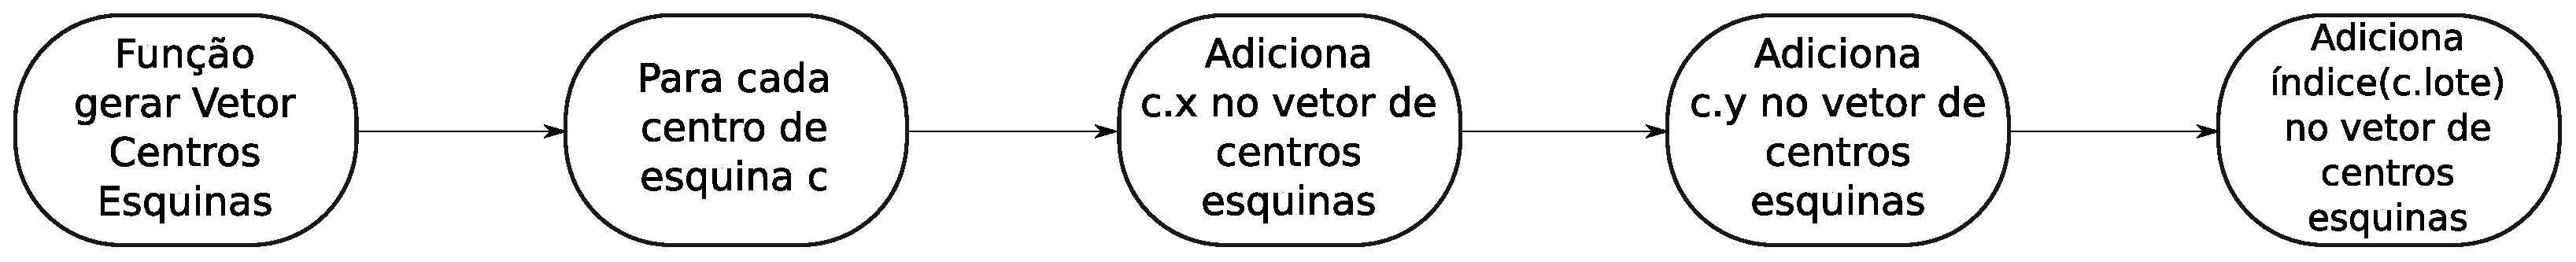
\includegraphics[width=1\textwidth]{Figuras/Simula/Fluxos/gerarVetorCentrosEsquinas.eps}
  \caption{Função gerarVetorCentrosEsquinas.}
  \label{fig:gerarVetorCentrosEsquinas}
\end{figure} 

\newpage

\subsubsection{Função getLotes}

O Código \ref{cod:getLotes}, Algoritmo \ref{alg:getLotes} e Figura \ref{fig:getLotes} ilustram a rotina responsável pela obtenção dos lotes do ambiente. Esta rotina realiza uma consulta ao banco de dados para obter as informações armazenadas na tabela com sufixo \textit{"\_lotes"}. A função de criação e um exemplo da tabela são ilustrados no Código \ref{cod:sql_getLotes} e Tabela \ref{tab:cascavel_lotes}.  

\lstinputlisting[caption=Função getLotes, label=cod:getLotes, captionpos=b, language=Java]{Codigos/Simula/Fontes/getLotes.java}

\begin{algorithm}[H]
   \SetAlgoLined   
   \input{Codigos/Simula/Algoritmos/getLotes.txt}
   \caption{\textsc{Função getLotes.}}
   \label{alg:getLotes}
\end{algorithm}

\begin{figure}[H]
  \centering
  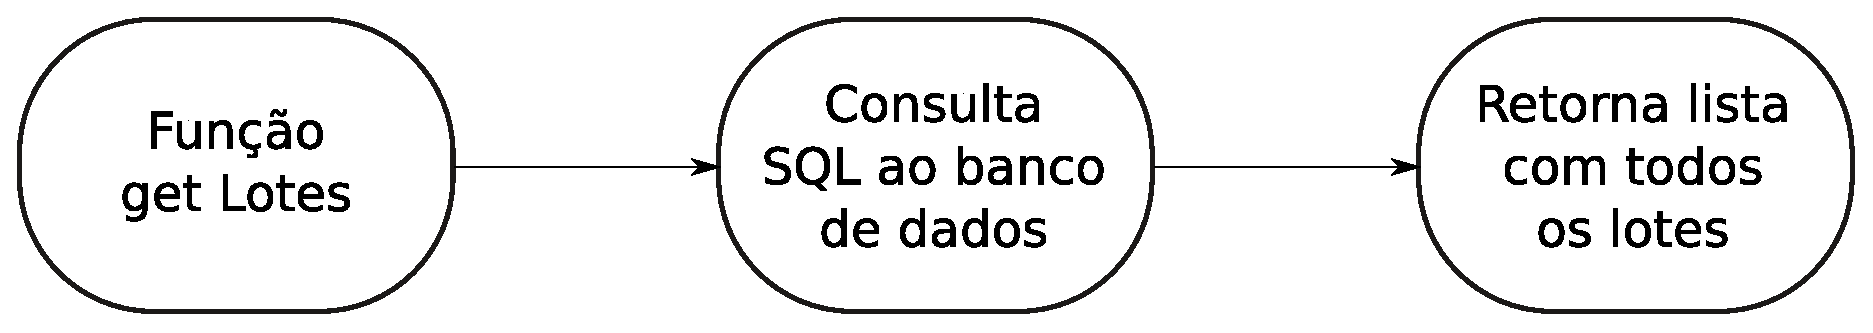
\includegraphics[width=0.7\textwidth]{Figuras/Simula/Fluxos/getLotes.eps}
  \caption{Função getLotes.}
  \label{fig:getLotes}
\end{figure} 

\newpage

\subsubsection{Função distribuirLocais}

O Código \ref{cod:distribuirLocais}, Algoritmo \ref{alg:distribuirLocais} e Figura \ref{fig:distribuirLocais} ilustram a rotina responsável pelas escolhas dos lotes representantes das casas e locais de trabalho, lazer e estudo. Um lote pode receber nenhuma ou exatamente uma atribuição de local. As escolhas dos locais são realizadas randomicamente por meio de sucessivos embaralhamentos e retiradas de elementos da estrutura que armazena todos os lotes. 

\lstinputlisting[caption=Função distribuirLocais, label=cod:distribuirLocais, captionpos=b, language=Java]{Codigos/Simula/Fontes/distribuirLocais.java}

\begin{algorithm}[H]
   \SetAlgoLined   
   \input{Codigos/Simula/Algoritmos/distribuirLocais.txt}
   \caption{\textsc{Função distribuirLocais.}}
   \label{alg:distribuirLocais}
\end{algorithm}

\begin{figure}[H]
  \centering
  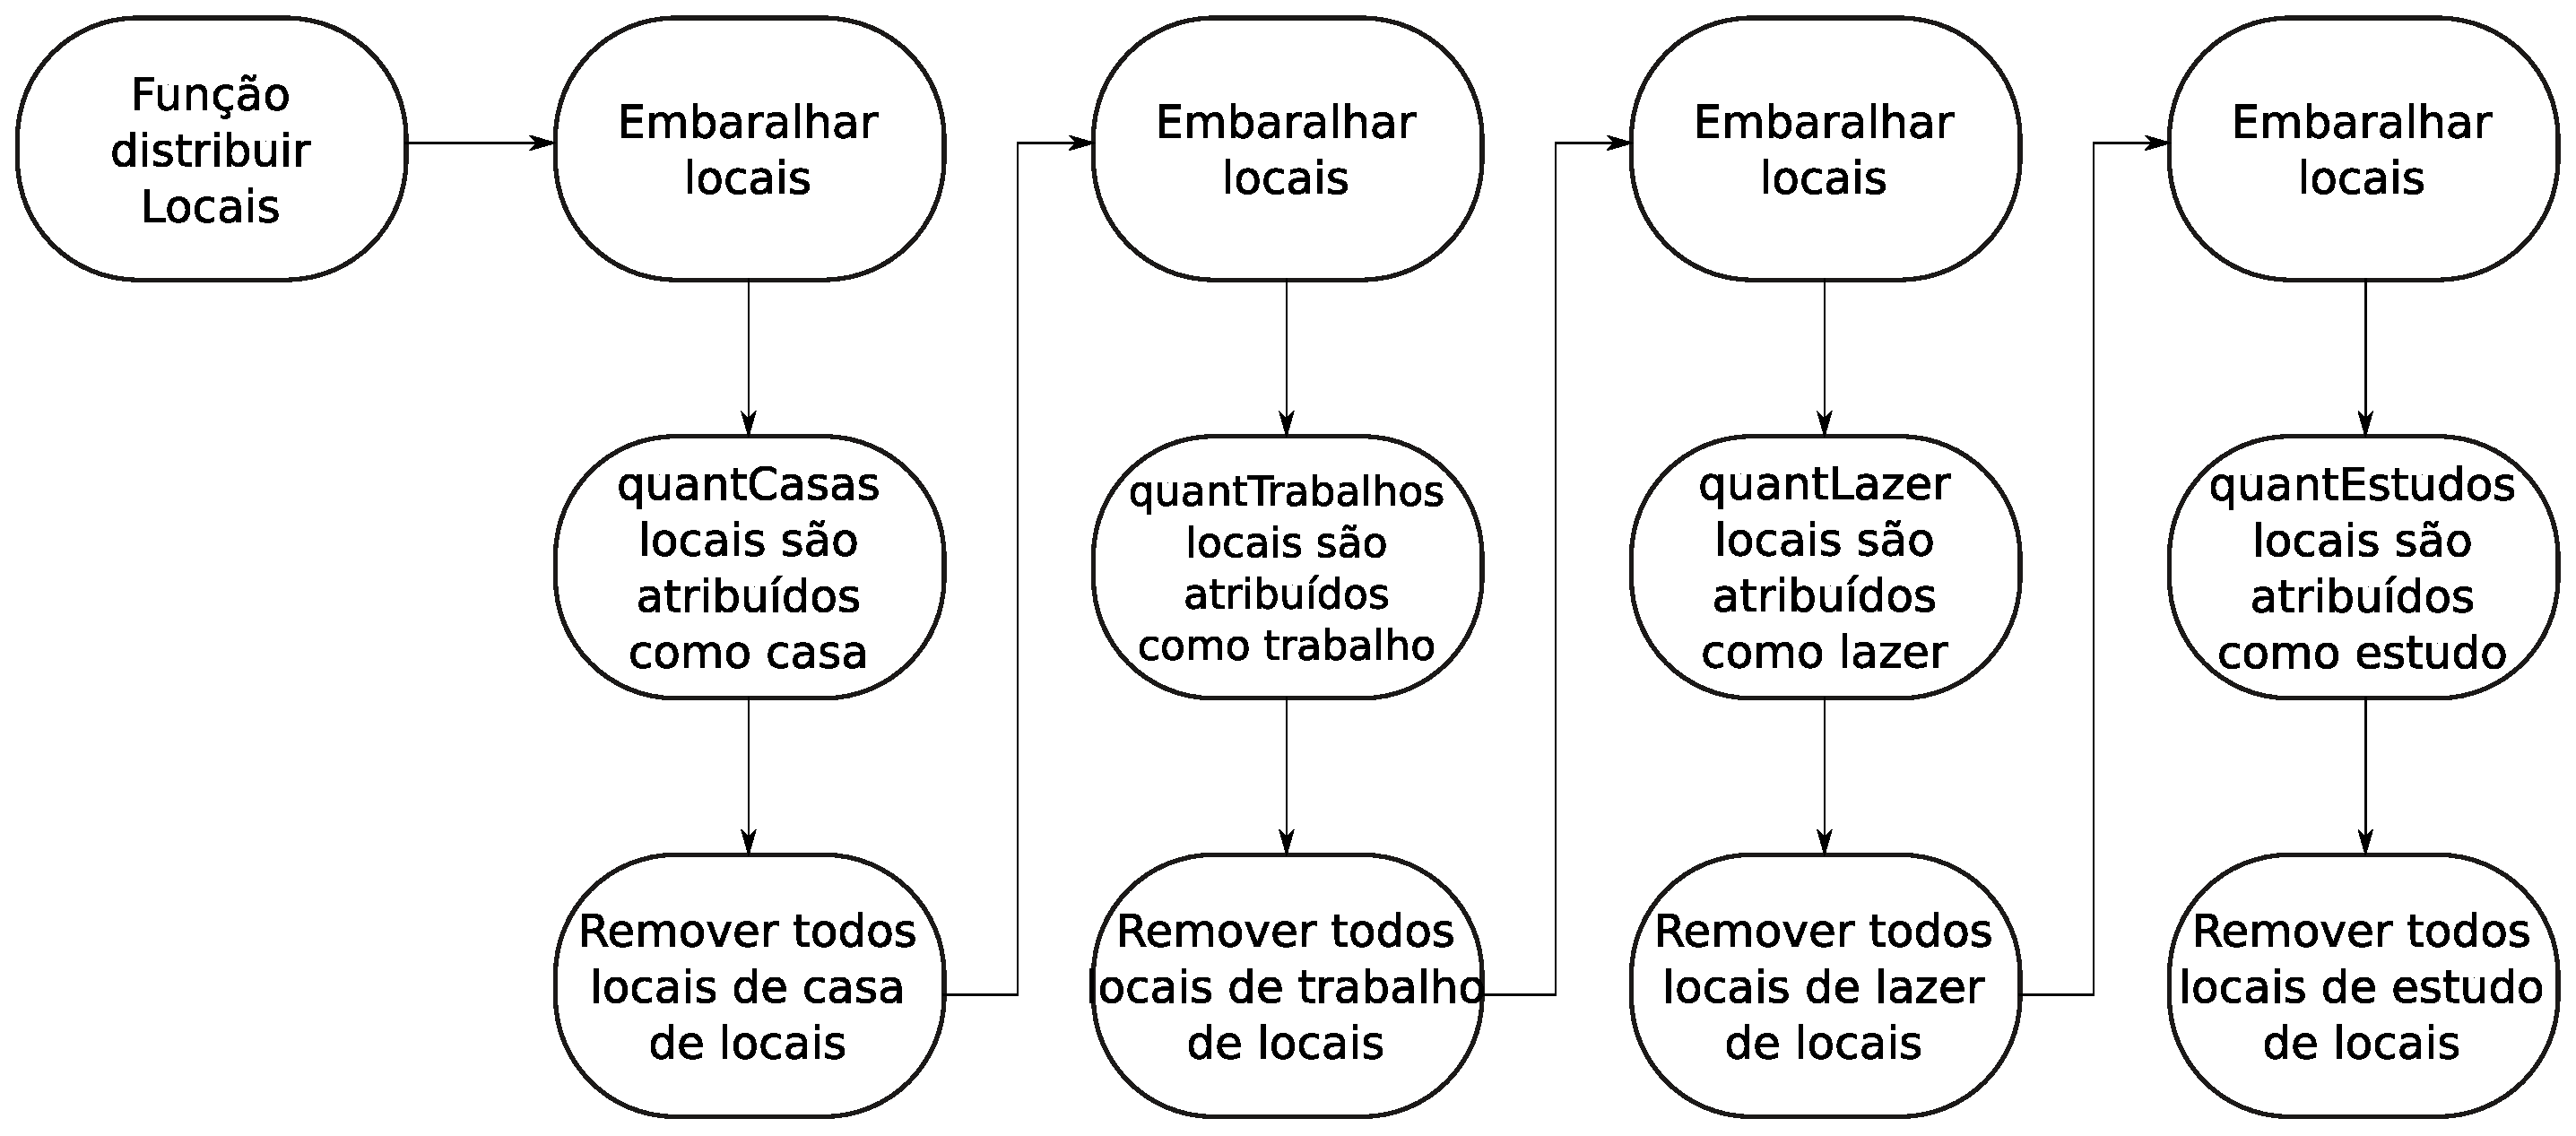
\includegraphics[width=0.8\textwidth]{Figuras/Simula/Fluxos/distribuirLocais.eps}
  \caption{Função distribuirLocais.}
  \label{fig:distribuirLocais}
\end{figure} 

\newpage

\subsubsection{Função gerarTrajetos}

O Código \ref{cod:gerarTrajetos}, Algoritmos \ref{alg:gerarTrajetos1}, \ref{alg:gerarTrajetos2}, \ref{alg:gerarTrajetos3} e \ref{alg:gerarTrajetos4} e Figura \ref{fig:gerarTrajetos} ilustram a rotina responsável pela geração dos trajetos às faixas etárias dos agentes. Para cada lote atribuído como casa pela rotina de distribuição de locais são gerados quatro trajetos, um para cada faixa etária. Como existem vários tipos de trajetos para cada faixa etária um deles é escolhido aleatoriamente e tomado como base. Do trajeto escolhido são utilizados os períodos de permanência e os tipos de locais. Os períodos de permanência são multiplicados pela duração do dia em ciclos, que é atualmente fixado em $100$. Os tipos de locais são utilizados à escolha aleatória dos locais pertencentes ao trajeto, exceto os locais de casa que já são conhecidos. 

\lstinputlisting[caption=Função gerarTrajetos, label=cod:gerarTrajetos, captionpos=b, language=Java]{Codigos/Simula/Fontes/gerarTrajetos.java}

\newpage

\begin{algorithm}[H]
   \SetAlgoLined   
   \input{Codigos/Simula/Algoritmos/gerarTrajetos1.txt}
   \caption{\textsc{Função gerarTrajetos - Parte I.}}
   \label{alg:gerarTrajetos1}
\end{algorithm}

\newpage

\begin{algorithm}[H]
   \SetAlgoLined   
   \input{Codigos/Simula/Algoritmos/gerarTrajetos2.txt}
   \caption{\textsc{Função gerarTrajetos - Parte II.}}
   \label{alg:gerarTrajetos2}
\end{algorithm}

\newpage

\begin{algorithm}[H]
   \SetAlgoLined   
   \input{Codigos/Simula/Algoritmos/gerarTrajetos3.txt}
   \caption{\textsc{Função gerarTrajetos - Parte III.}}
   \label{alg:gerarTrajetos3}
\end{algorithm}

\newpage

\begin{algorithm}[H]
   \SetAlgoLined   
   \input{Codigos/Simula/Algoritmos/gerarTrajetos4.txt}
   \caption{\textsc{Função gerarTrajetos - Parte IV.}}
   \label{alg:gerarTrajetos4}
\end{algorithm}

\begin{figure}[H]
  \centering
  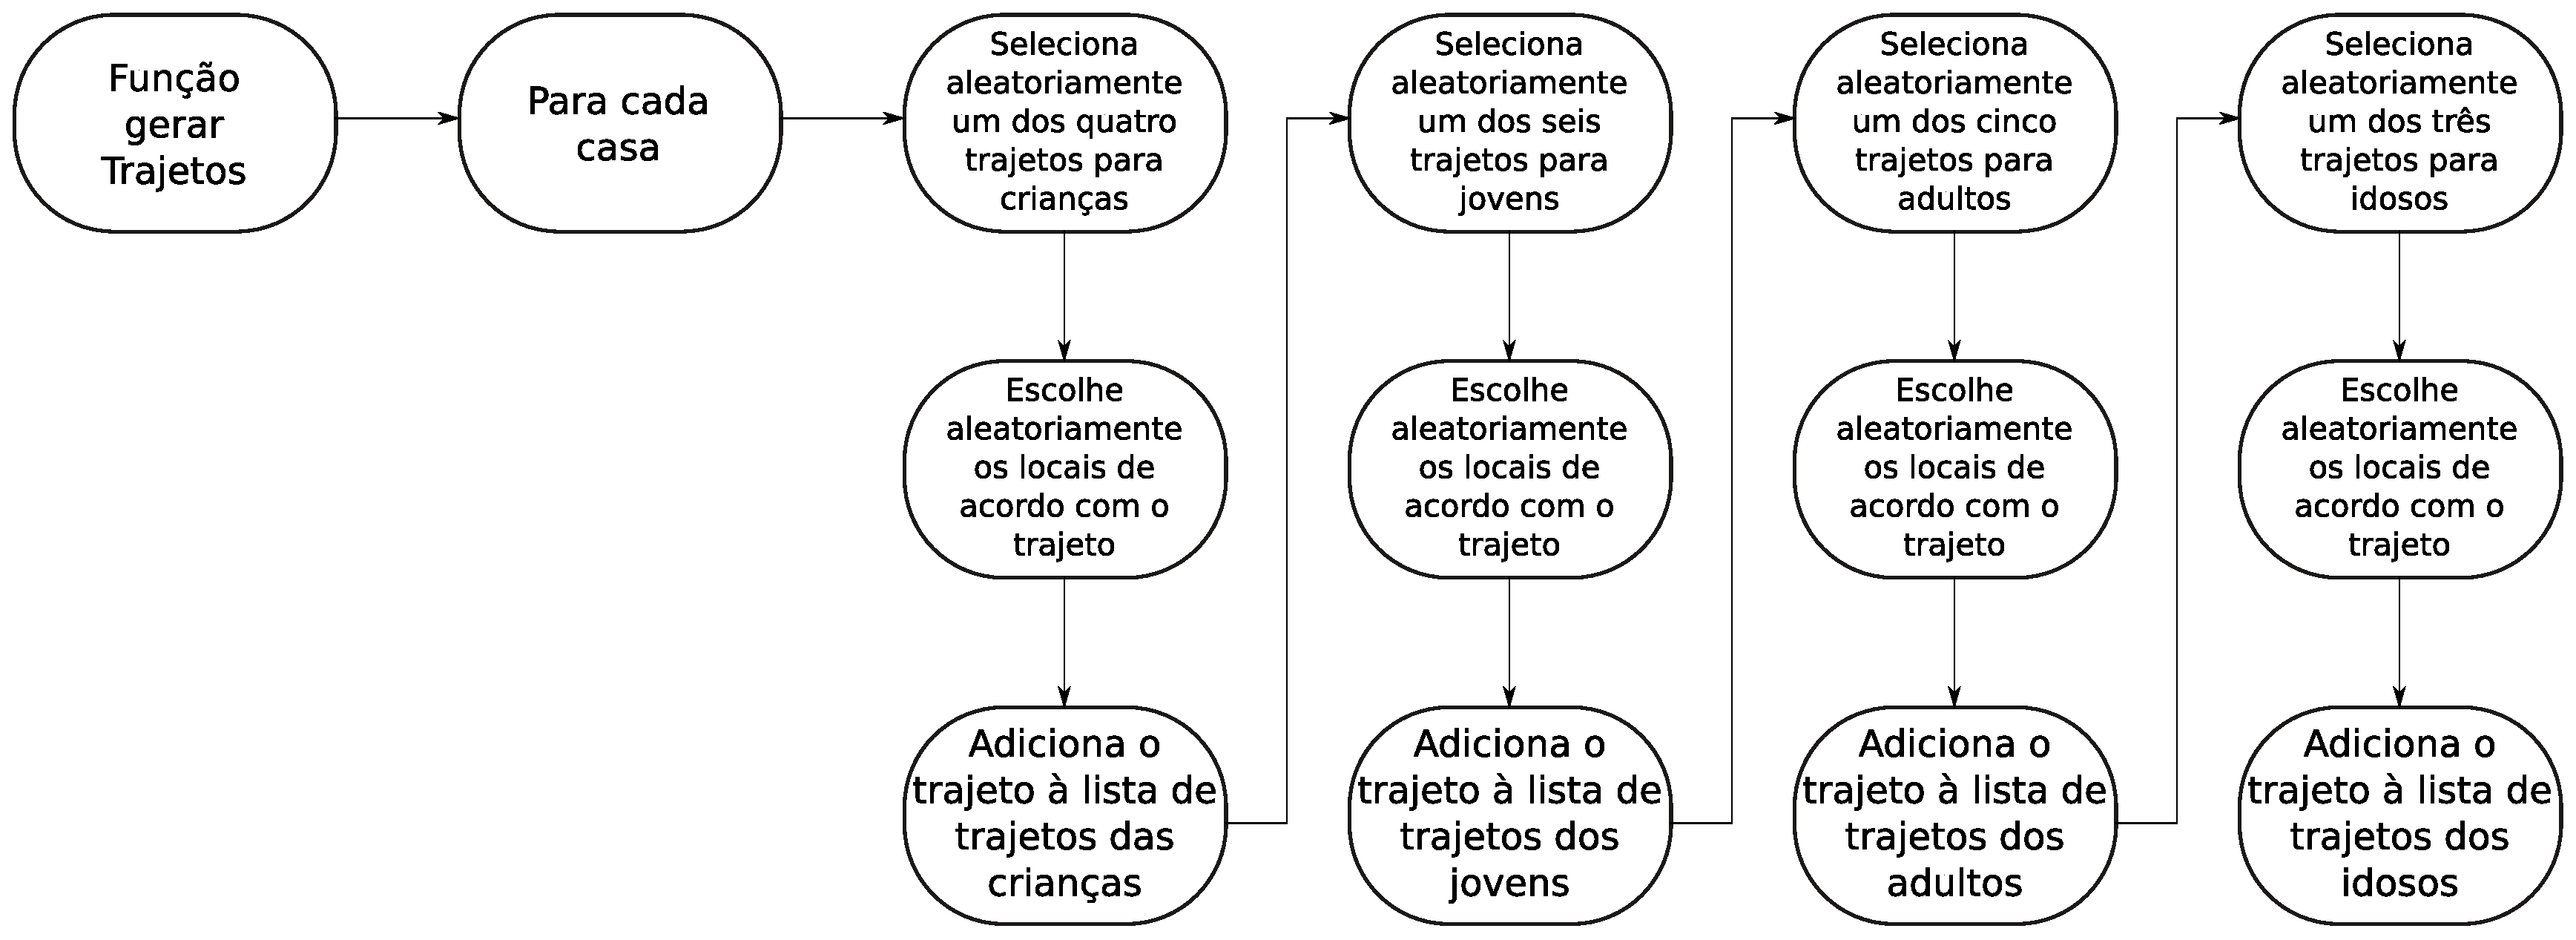
\includegraphics[width=0.9\textwidth]{Figuras/Simula/Fluxos/gerarTrajetos.eps}
  \caption{Função gerarTrajetos.}
  \label{fig:gerarTrajetos}
\end{figure} 

\newpage

\subsubsection{Função getArestas}

O Código \ref{cod:getArestas}, Algoritmo \ref{alg:getArestas} e Figura \ref{fig:getArestas} ilustram a rotina responsável pela obtenção das arestas entre os polígonos do ambiente. Esta rotina realiza uma consulta ao banco de dados para obter as informações armazenadas na tabela com sufixo \textit{"\_arestas"}. A função de criação e um exemplo da tabela são ilustrados no Código \ref{cod:sql_getArestas} e Tabela \ref{tab:cascavel_arestas}.  

\lstinputlisting[caption=Função getArestas, label=cod:getArestas, captionpos=b, language=Java]{Codigos/Simula/Fontes/getArestas.java}

\begin{algorithm}[H]
   \SetAlgoLined   
   \input{Codigos/Simula/Algoritmos/getArestas.txt}
   \caption{\textsc{Função getArestas.}}
   \label{alg:getArestas}
\end{algorithm}

\begin{figure}[H]
  \centering
  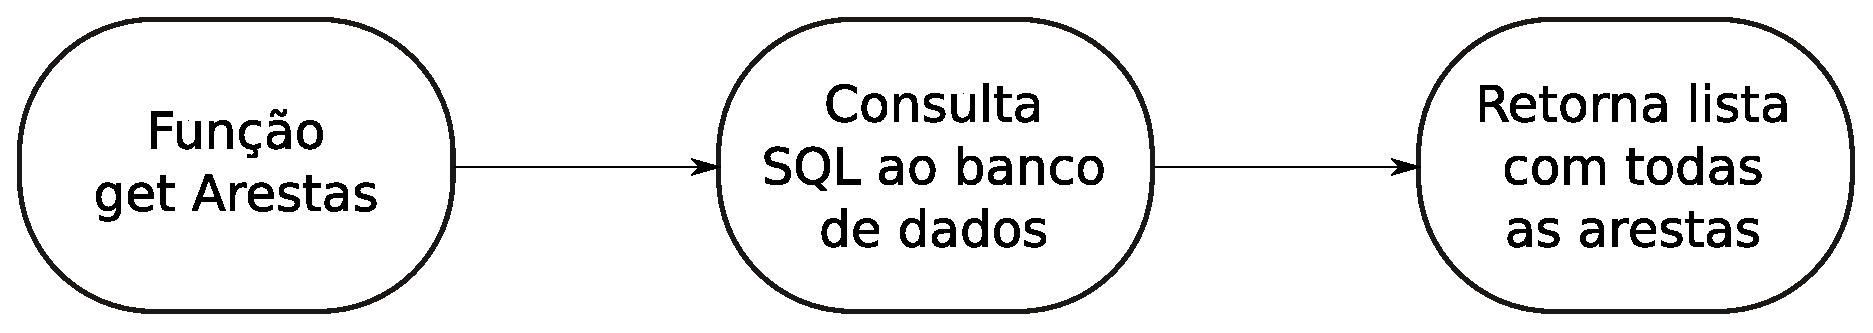
\includegraphics[width=0.7\textwidth]{Figuras/Simula/Fluxos/getArestas.eps}
  \caption{Função getArestas.}
  \label{fig:getArestas}
\end{figure} 

\newpage

\subsubsection{Função getCentroidesEsquinas}

O Código \ref{cod:getCentroidesEsquinas}, Algoritmo \ref{alg:getCentroidesEsquinas} e Figura \ref{fig:getCentroidesEsquinas} ilustram a rotina responsável pela obtenção dos vértices centros das esquinas. Esta rotina realiza uma consulta ao banco de dados para obter as informações armazenadas na tabela com sufixo \textit{"\_centroidesesquinas"}. A função de criação e um exemplo da tabela são ilustrados no Código \ref{cod:sql_getCentroidesEsquinas} e Tabela \ref{tab:cascavel_centroidesesquinas}. 

\lstinputlisting[caption=Função getCentroidesEsquinas, label=cod:getCentroidesEsquinas, captionpos=b, language=Java]{Codigos/Simula/Fontes/getCentroidesEsquinas.java}

\begin{algorithm}[H]
   \SetAlgoLined   
   \input{Codigos/Simula/Algoritmos/getCentroidesEsquinas.txt}
   \caption{\textsc{Função getCentroidesEsquinas.}}
   \label{alg:getCentroidesEsquinas}
\end{algorithm}

\begin{figure}[H]
  \centering
  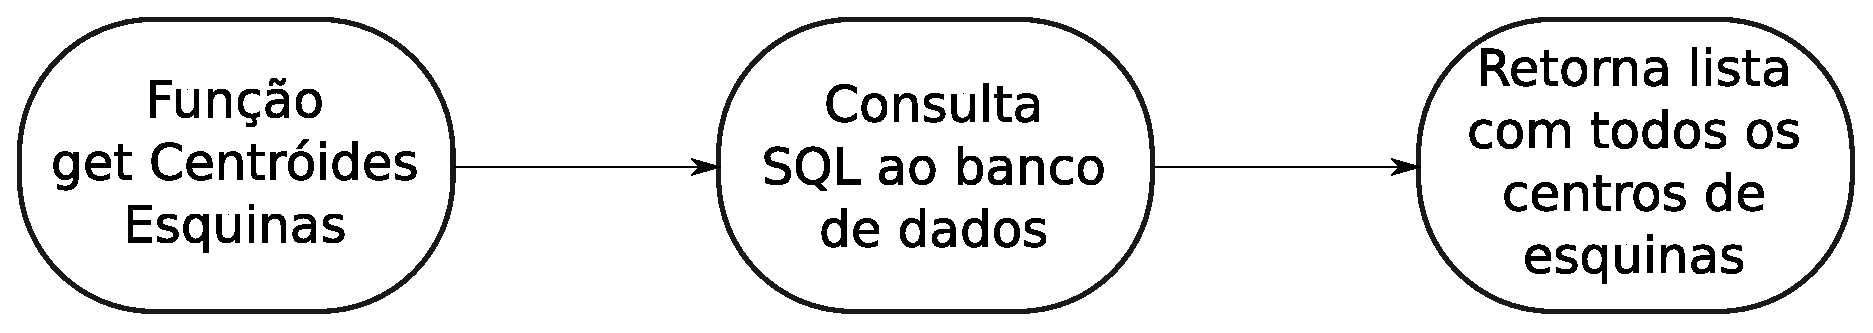
\includegraphics[width=0.7\textwidth]{Figuras/Simula/Fluxos/getCentroidesEsquinas.eps}
  \caption{Função getCentroidesEsquinas.}
  \label{fig:getCentroidesEsquinas}
\end{figure} 

\newpage

\subsubsection{Função getCentroidesLotes}

O Código \ref{cod:getCentroidesLotes}, Algoritmo \ref{alg:getCentroidesLotes} e Figura \ref{fig:getCentroidesLotes} ilustram a rotina responsável pela obtenção dos vértices centros dos lotes do ambiente de simulação. Esta rotina realiza uma consulta ao banco de dados para obter as informações armazenadas na tabela com sufixo \textit{"\_centroideslotes"}. A função de criação e um exemplo da tabela são ilustrados no Código \ref{cod:sql_getCentroidesLotes} e Tabela \ref{tab:cascavel_centroideslotes}. 

\lstinputlisting[caption=Função getCentroidesLotes, label=cod:getCentroidesLotes, captionpos=b, language=Java]{Codigos/Simula/Fontes/getCentroidesLotes.java}

\begin{algorithm}[H]
   \SetAlgoLined   
   \input{Codigos/Simula/Algoritmos/getCentroidesLotes.txt}
   \caption{\textsc{Função getCentroidesLotes.}}
   \label{alg:getCentroidesLotes}
\end{algorithm}

\begin{figure}[H]
  \centering
  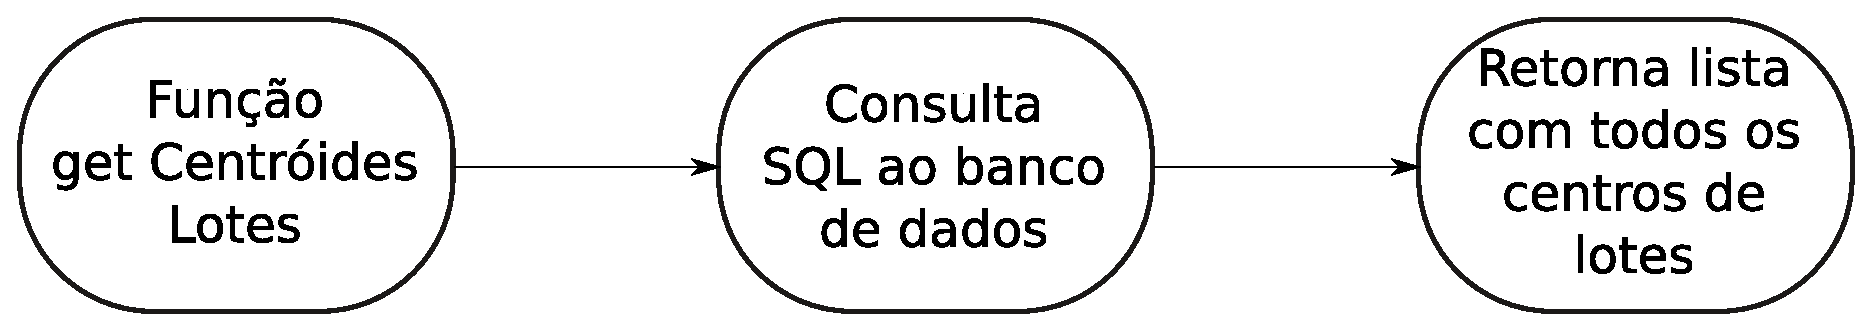
\includegraphics[width=0.7\textwidth]{Figuras/Simula/Fluxos/getCentroidesLotes.eps}
  \caption{Função getCentroidesLotes.}
  \label{fig:getCentroidesLotes}
\end{figure} 

\newpage

\subsubsection{Função getVertices}

O Código \ref{cod:getVertices}, Algoritmo \ref{alg:getVertices} e Figura \ref{fig:getVertices} ilustram a rotina responsável pela obtenção dos vértices do ambiente, que são neste contexto todos os polígonos de ruas e lotes. Esta rotina realiza uma consulta ao banco de dados para obter as informações armazenadas na tabela com sufixo \textit{"\_vertices"}. A função de criação e um exemplo da tabela são ilustrados no Código \ref{cod:sql_getVertices} e Tabela \ref{tab:cascavel_vertices}. 

\lstinputlisting[caption=Função getVertices, label=cod:getVertices, captionpos=b, language=Java]{Codigos/Simula/Fontes/getVertices.java}

\begin{algorithm}[H]
   \SetAlgoLined   
   \input{Codigos/Simula/Algoritmos/getVertices.txt}
   \caption{\textsc{Função getVertices.}}
   \label{alg:getVertices}
\end{algorithm}

\begin{figure}[H]
  \centering
  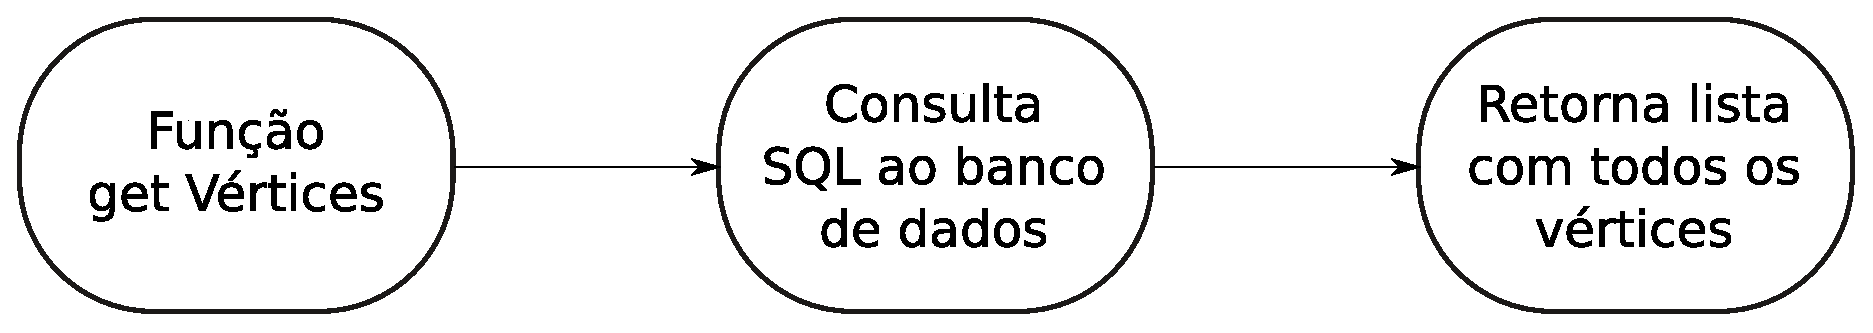
\includegraphics[width=0.7\textwidth]{Figuras/Simula/Fluxos/getVertices.eps}
  \caption{Função getVertices.}
  \label{fig:getVertices}
\end{figure} 

\newpage

\subsubsection{Função gerarCaminhos}

O Código \ref{cod:gerarCaminhos}, Algoritmo \ref{alg:gerarCaminhos} e Figura \ref{fig:gerarCaminhos} ilustram a rotina responsável pela geração dos caminhos. Os caminhos são as listas de ruas que pertencem às rotas. Para cada rota pertencente à cada trajeto o algoritmo A* é executado, retornando como resultado a lista de ruas que devem ser percorridas pelo agente para deslocar-se de um lote origem à um lote destino. Posteriormente estas informações são utilizadas na composição da estrutura que armazena as rotas. 

\lstinputlisting[caption=Função gerarCaminhos, label=cod:gerarCaminhos, captionpos=b, language=Java]{Codigos/Simula/Fontes/gerarCaminhos.java}

\begin{algorithm}[H]
   \SetAlgoLined   
   \input{Codigos/Simula/Algoritmos/gerarCaminhos.txt}
   \caption{\textsc{Função gerarCaminhos.}}
   \label{alg:gerarCaminhos}
\end{algorithm}

\begin{figure}[H]
  \centering
  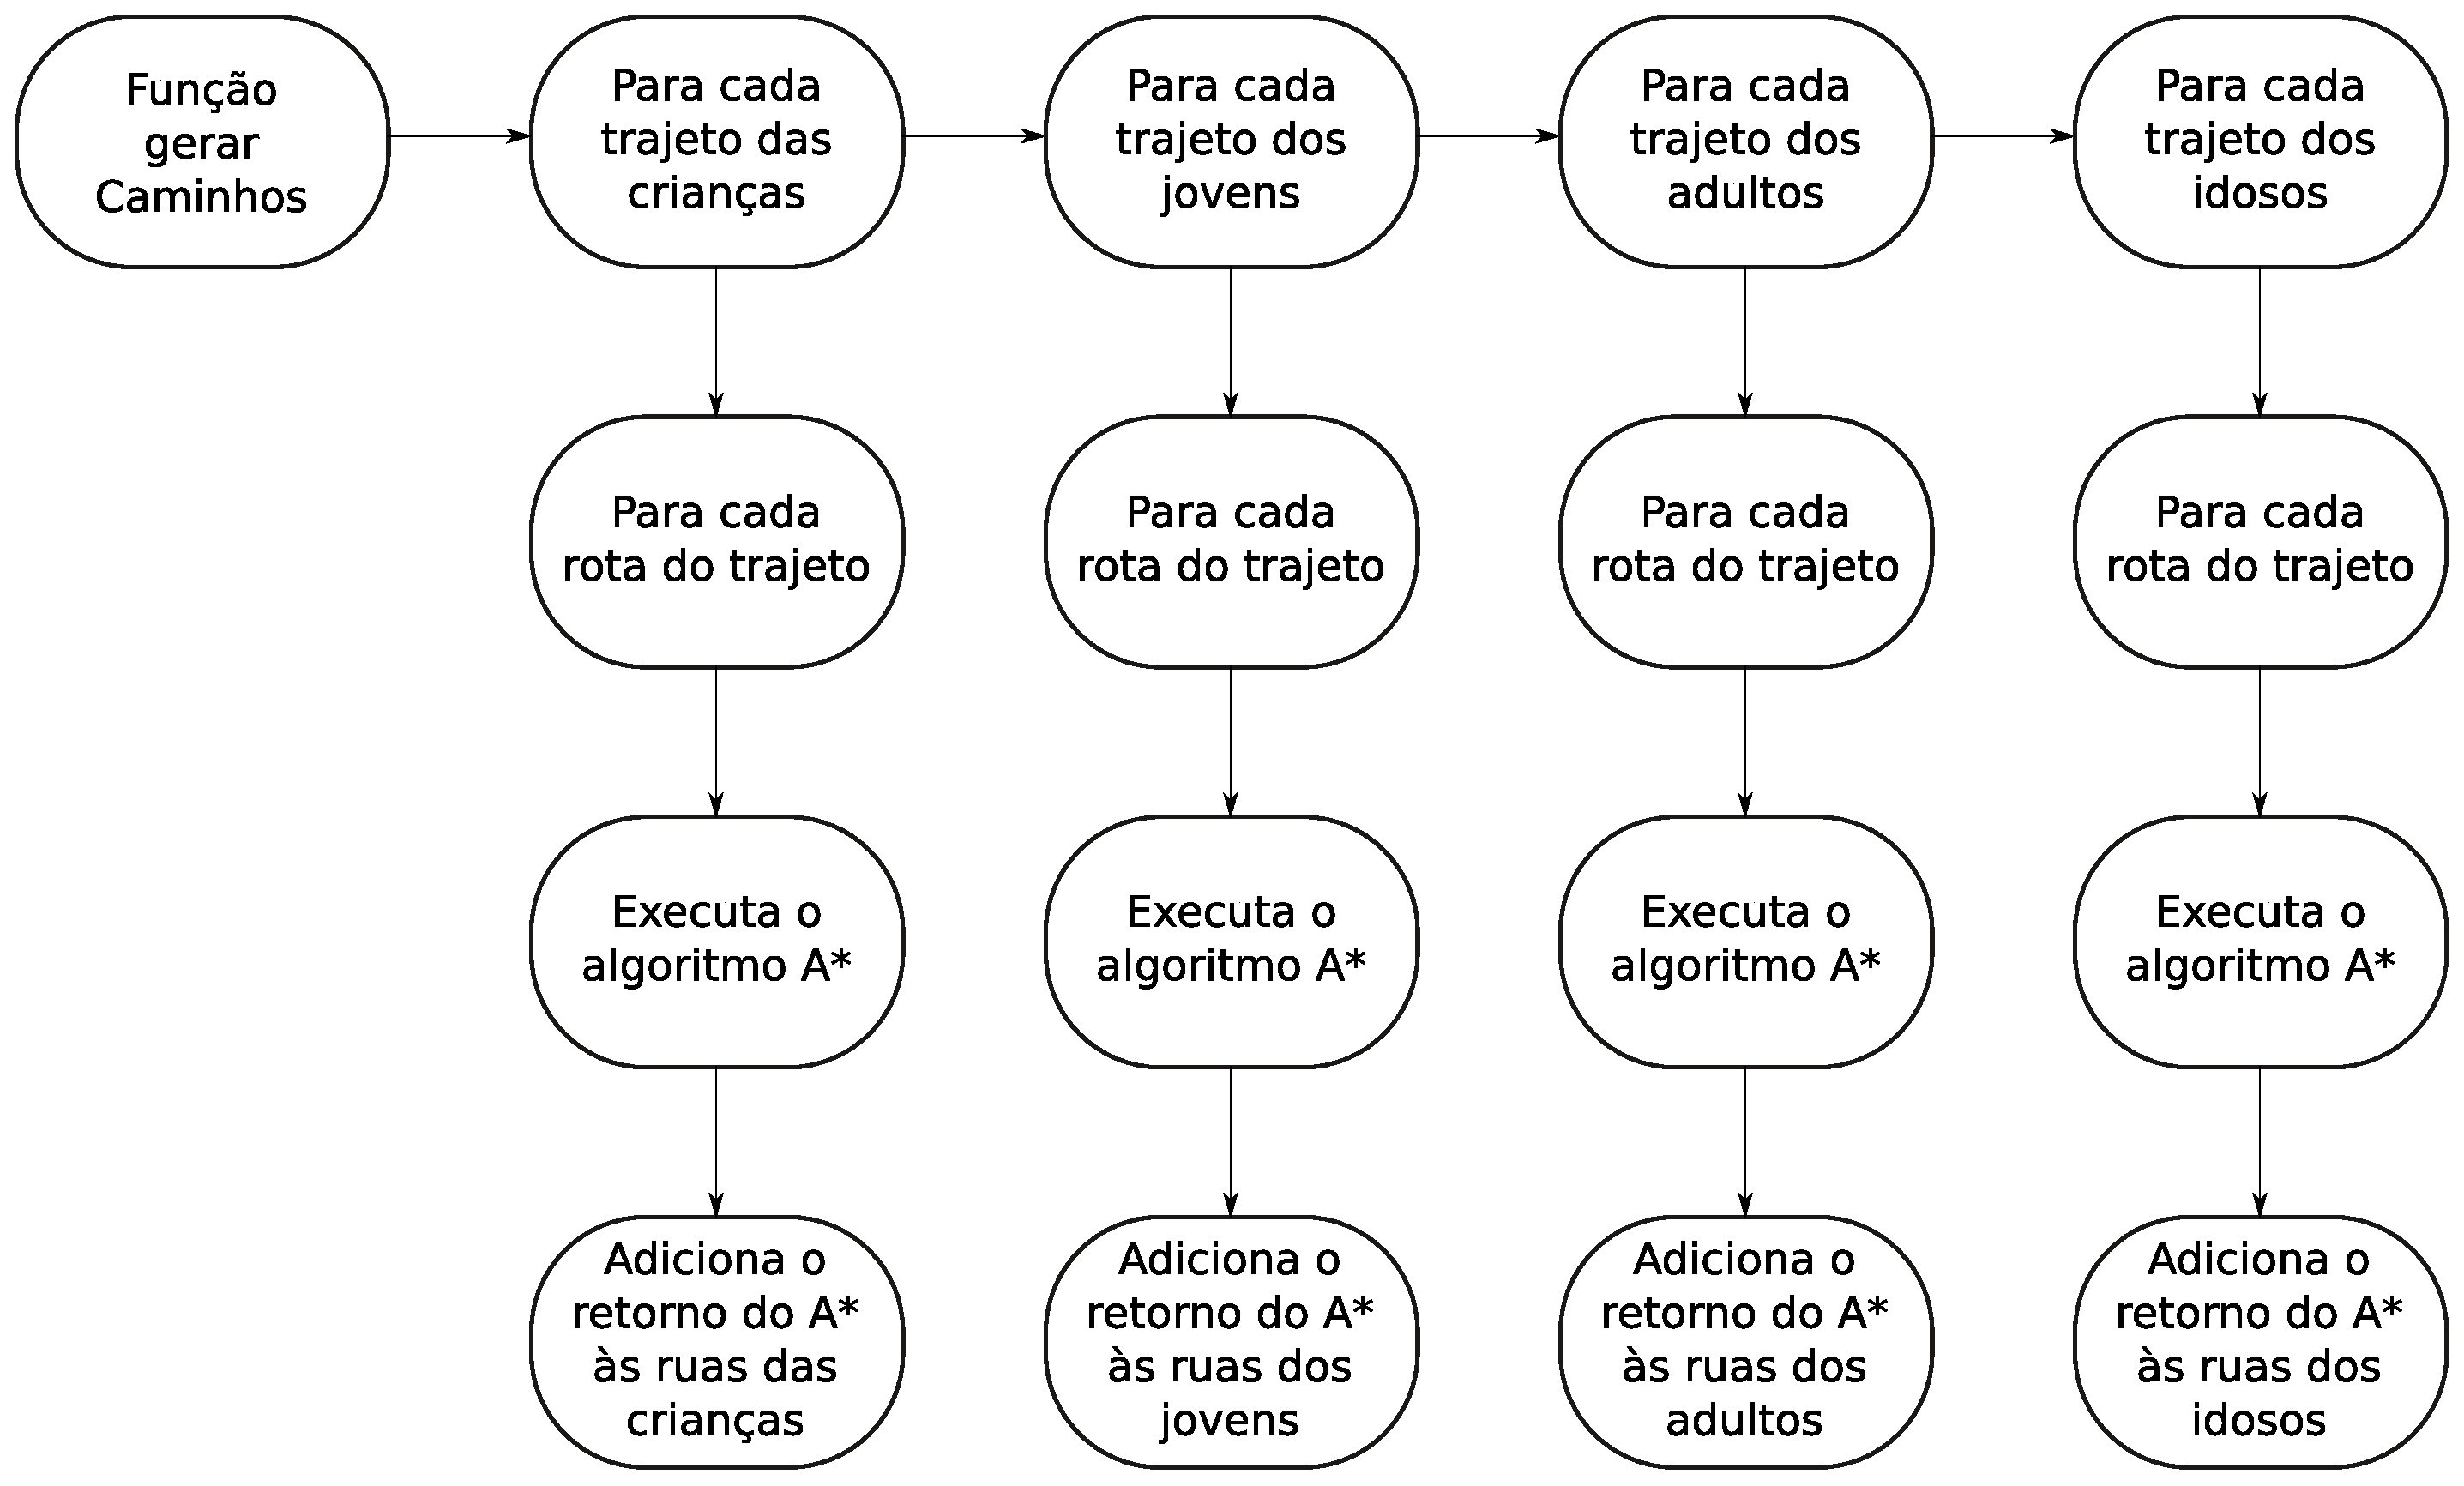
\includegraphics[width=0.8\textwidth]{Figuras/Simula/Fluxos/gerarCaminhos.eps}
  \caption{Função gerarCaminhos.}
  \label{fig:gerarCaminhos}
\end{figure} 

\newpage

\subsubsection{Função aEstrela}

O Código \ref{cod:aEstrela}, Algoritmo \ref{alg:aEstrela} e \ref{fig:aEstrela} ilustram o algoritmo A* implementado à busca dos caminhos entre dois lotes de uma rota. O algoritmo original foi adaptado para adequar-se corretamente ao problema. Somente os lotes pertencentes às ruas são considerados como vértices possíveis à formação do caminho, já que os agentes devem deslocar-se somente pelas ruas até que alcancem o lote destino. Os pontos centro dos polígonos das ruas e dos lotes de origem e destino são utilizados ao cálculo das distâncias euclidianas, que é a heurística empregada no algoritmo. A heurística somente não é utilizada na escolha da primeira rota da rua, que é escolhida aleatoriamente. O algoritmo utiliza como entrada o grafo formado pelos vértices e arestas provenientes da execução das consultas apresentadas nos Códigos \ref{cod:sql_getVertices} e \ref{cod:sql_getArestas} e das funções apresentadas nos Códigos \ref{cod:getVertices} e \ref{cod:getArestas}.

\lstinputlisting[caption=Função aEstrela, label=cod:aEstrela, captionpos=b, language=Java]{Codigos/Simula/Fontes/aEstrela.java}

\begin{algorithm}[H]
   \SetAlgoLined   
   \input{Codigos/Simula/Algoritmos/aEstrela.txt}
   \caption{\textsc{Função aEstrela.}}
   \label{alg:aEstrela}
\end{algorithm}

\begin{figure}[H]
  \centering
  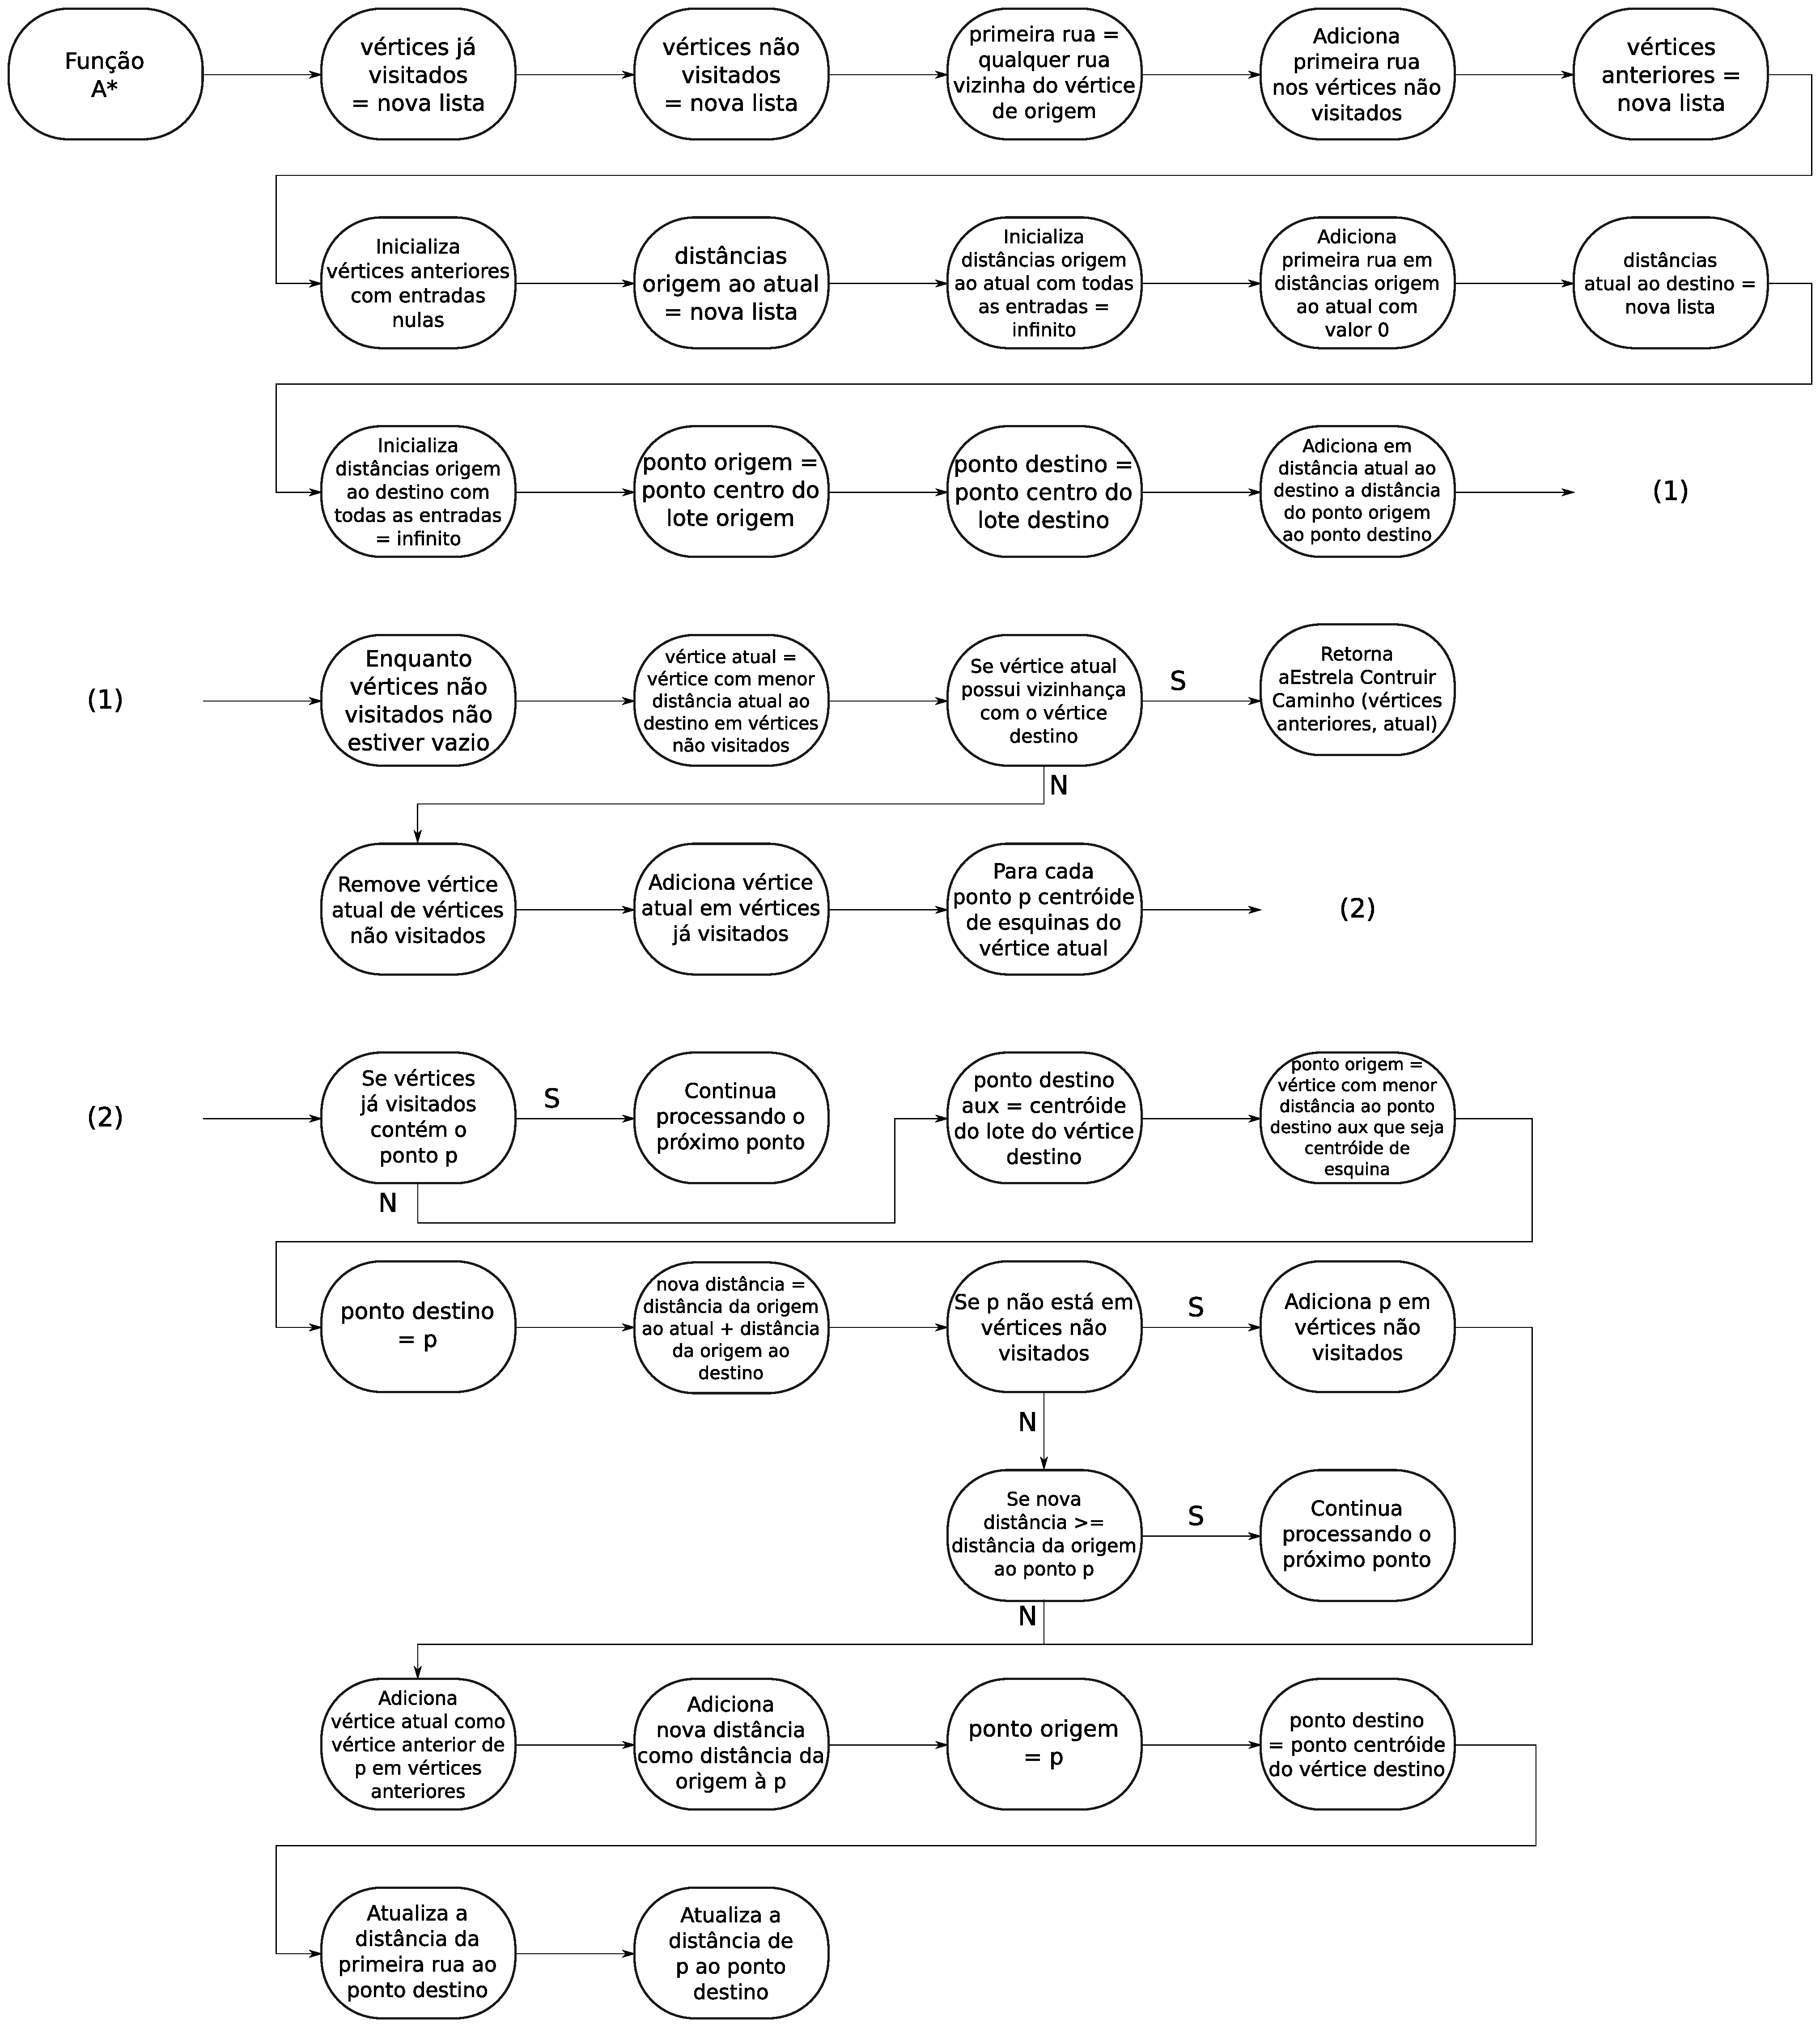
\includegraphics[width=1\textwidth]{Figuras/Simula/Fluxos/aEstrela.eps}
  \caption{Função aEstrela.}
  \label{fig:aEstrela}
\end{figure} 

\newpage

\subsubsection{Função aEstrelaConstruirCaminho}

O Código \ref{cod:aEstrelaConstruirCaminho}, Algoritmo \ref{alg:aEstrelaConstruirCaminho} e Figura \ref{fig:aEstrelaConstruirCaminho} ilustram a rotina responsável pela reconstrução do caminho encontrado pelo algoritmo A*. A rotina reconstrói o caminho retroativamente, partindo do vértice destino, utilizando informações mantidas pelo próprio algoritmo A* durante o processo de busca.

\lstinputlisting[caption=Função aEstrelaConstruirCaminho, label=cod:aEstrelaConstruirCaminho, captionpos=b, language=Java]{Codigos/Simula/Fontes/aEstrelaConstruirCaminho.java}

\begin{algorithm}[H]
   \SetAlgoLined
   \input{Codigos/Simula/Algoritmos/aEstrelaConstruirCaminho.txt}
   \caption{\textsc{Função aEstrelaConstruirCaminho.}}
   \label{alg:aEstrelaConstruirCaminho}
\end{algorithm}

\begin{figure}[H]
  \centering
  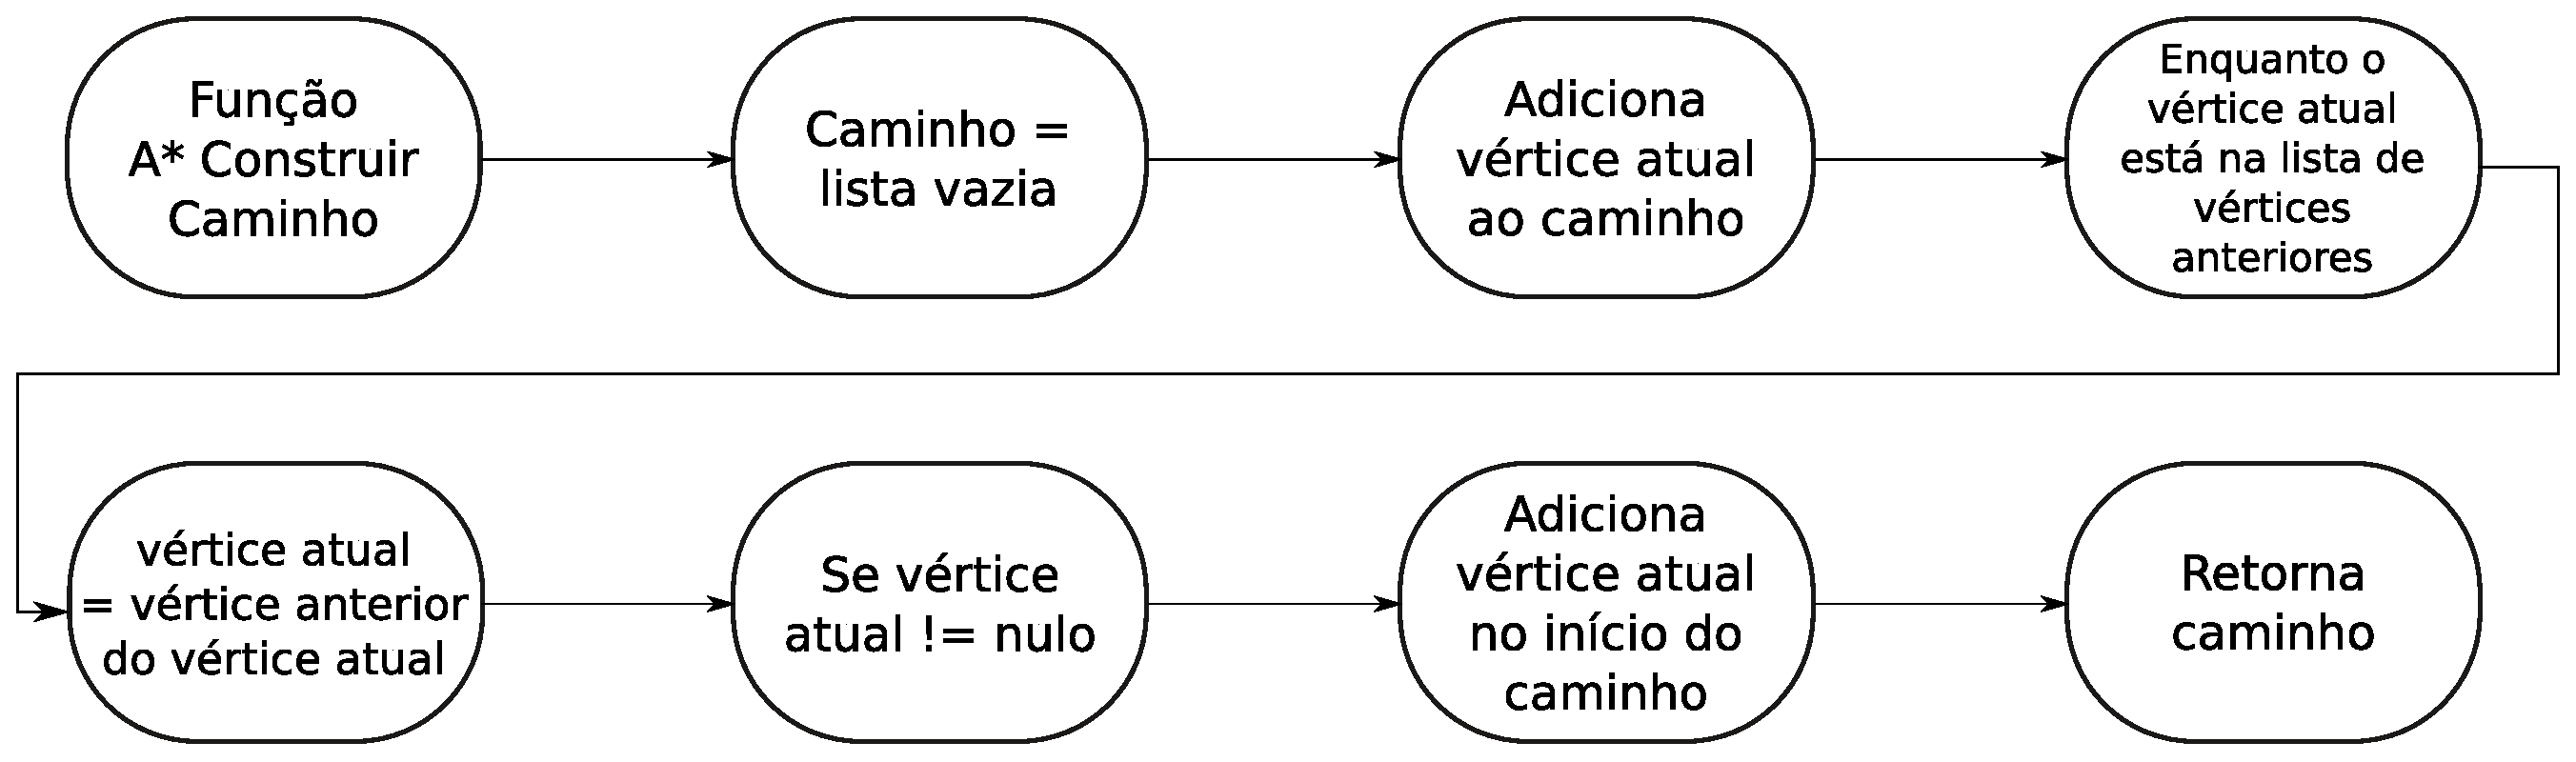
\includegraphics[width=0.9\textwidth]{Figuras/Simula/Fluxos/aEstrelaConstruirCaminho.eps}
  \caption{Função aEstrelaConstruirCaminho.}
  \label{fig:aEstrelaConstruirCaminho}
\end{figure} 

\newpage

\subsubsection{Função gerarVetorIndexRotas}

O Código \ref{cod:gerarVetorIndexRotas}, Algoritmos \ref{alg:gerarVetorIndexRotas1}, \ref{alg:gerarVetorIndexRotas2} e \ref{alg:gerarVetorIndexRotas3} e Figura \ref{fig:gerarVetorIndexRotas} ilustram a rotina responsável pela geração dos índices e do vetor das rotas. As rotas são utilizadas na rotina de movimentação em trajetos dos agentes. Em uma rota são armazenadas a quadra e lote de origem, a lista de ruas e a quadra e lote de destino. A lista de ruas descreve a sequência de ruas que o agente deve percorrer para chegar ao lote destino partindo do lote origem. Os índices especificam as posições de início e término de cada rota. 

\lstinputlisting[caption=Função gerarVetorIndexRotas, label=cod:gerarVetorIndexRotas, captionpos=b, language=Java]{Codigos/Simula/Fontes/gerarVetorIndexRotas.java}

\begin{algorithm}[H]
   \SetAlgoLined   
   \input{Codigos/Simula/Algoritmos/gerarVetorIndexRotas1.txt}
   \caption{\textsc{Função gerarVetorIndexRotas - Parte I.}}
   \label{alg:gerarVetorIndexRotas1}
\end{algorithm}

\newpage

\begin{algorithm}[H]
   \SetAlgoLined   
   \input{Codigos/Simula/Algoritmos/gerarVetorIndexRotas2.txt}
   \caption{\textsc{Função gerarVetorIndexRotas - Parte II.}}
   \label{alg:gerarVetorIndexRotas2}
\end{algorithm}

\newpage

\begin{algorithm}[H]
   \SetAlgoLined   
   \input{Codigos/Simula/Algoritmos/gerarVetorIndexRotas3.txt}
   \caption{\textsc{Função gerarVetorIndexRotas - Parte III.}}
   \label{alg:gerarVetorIndexRotas3}
\end{algorithm}

\begin{figure}[H]
  \centering
  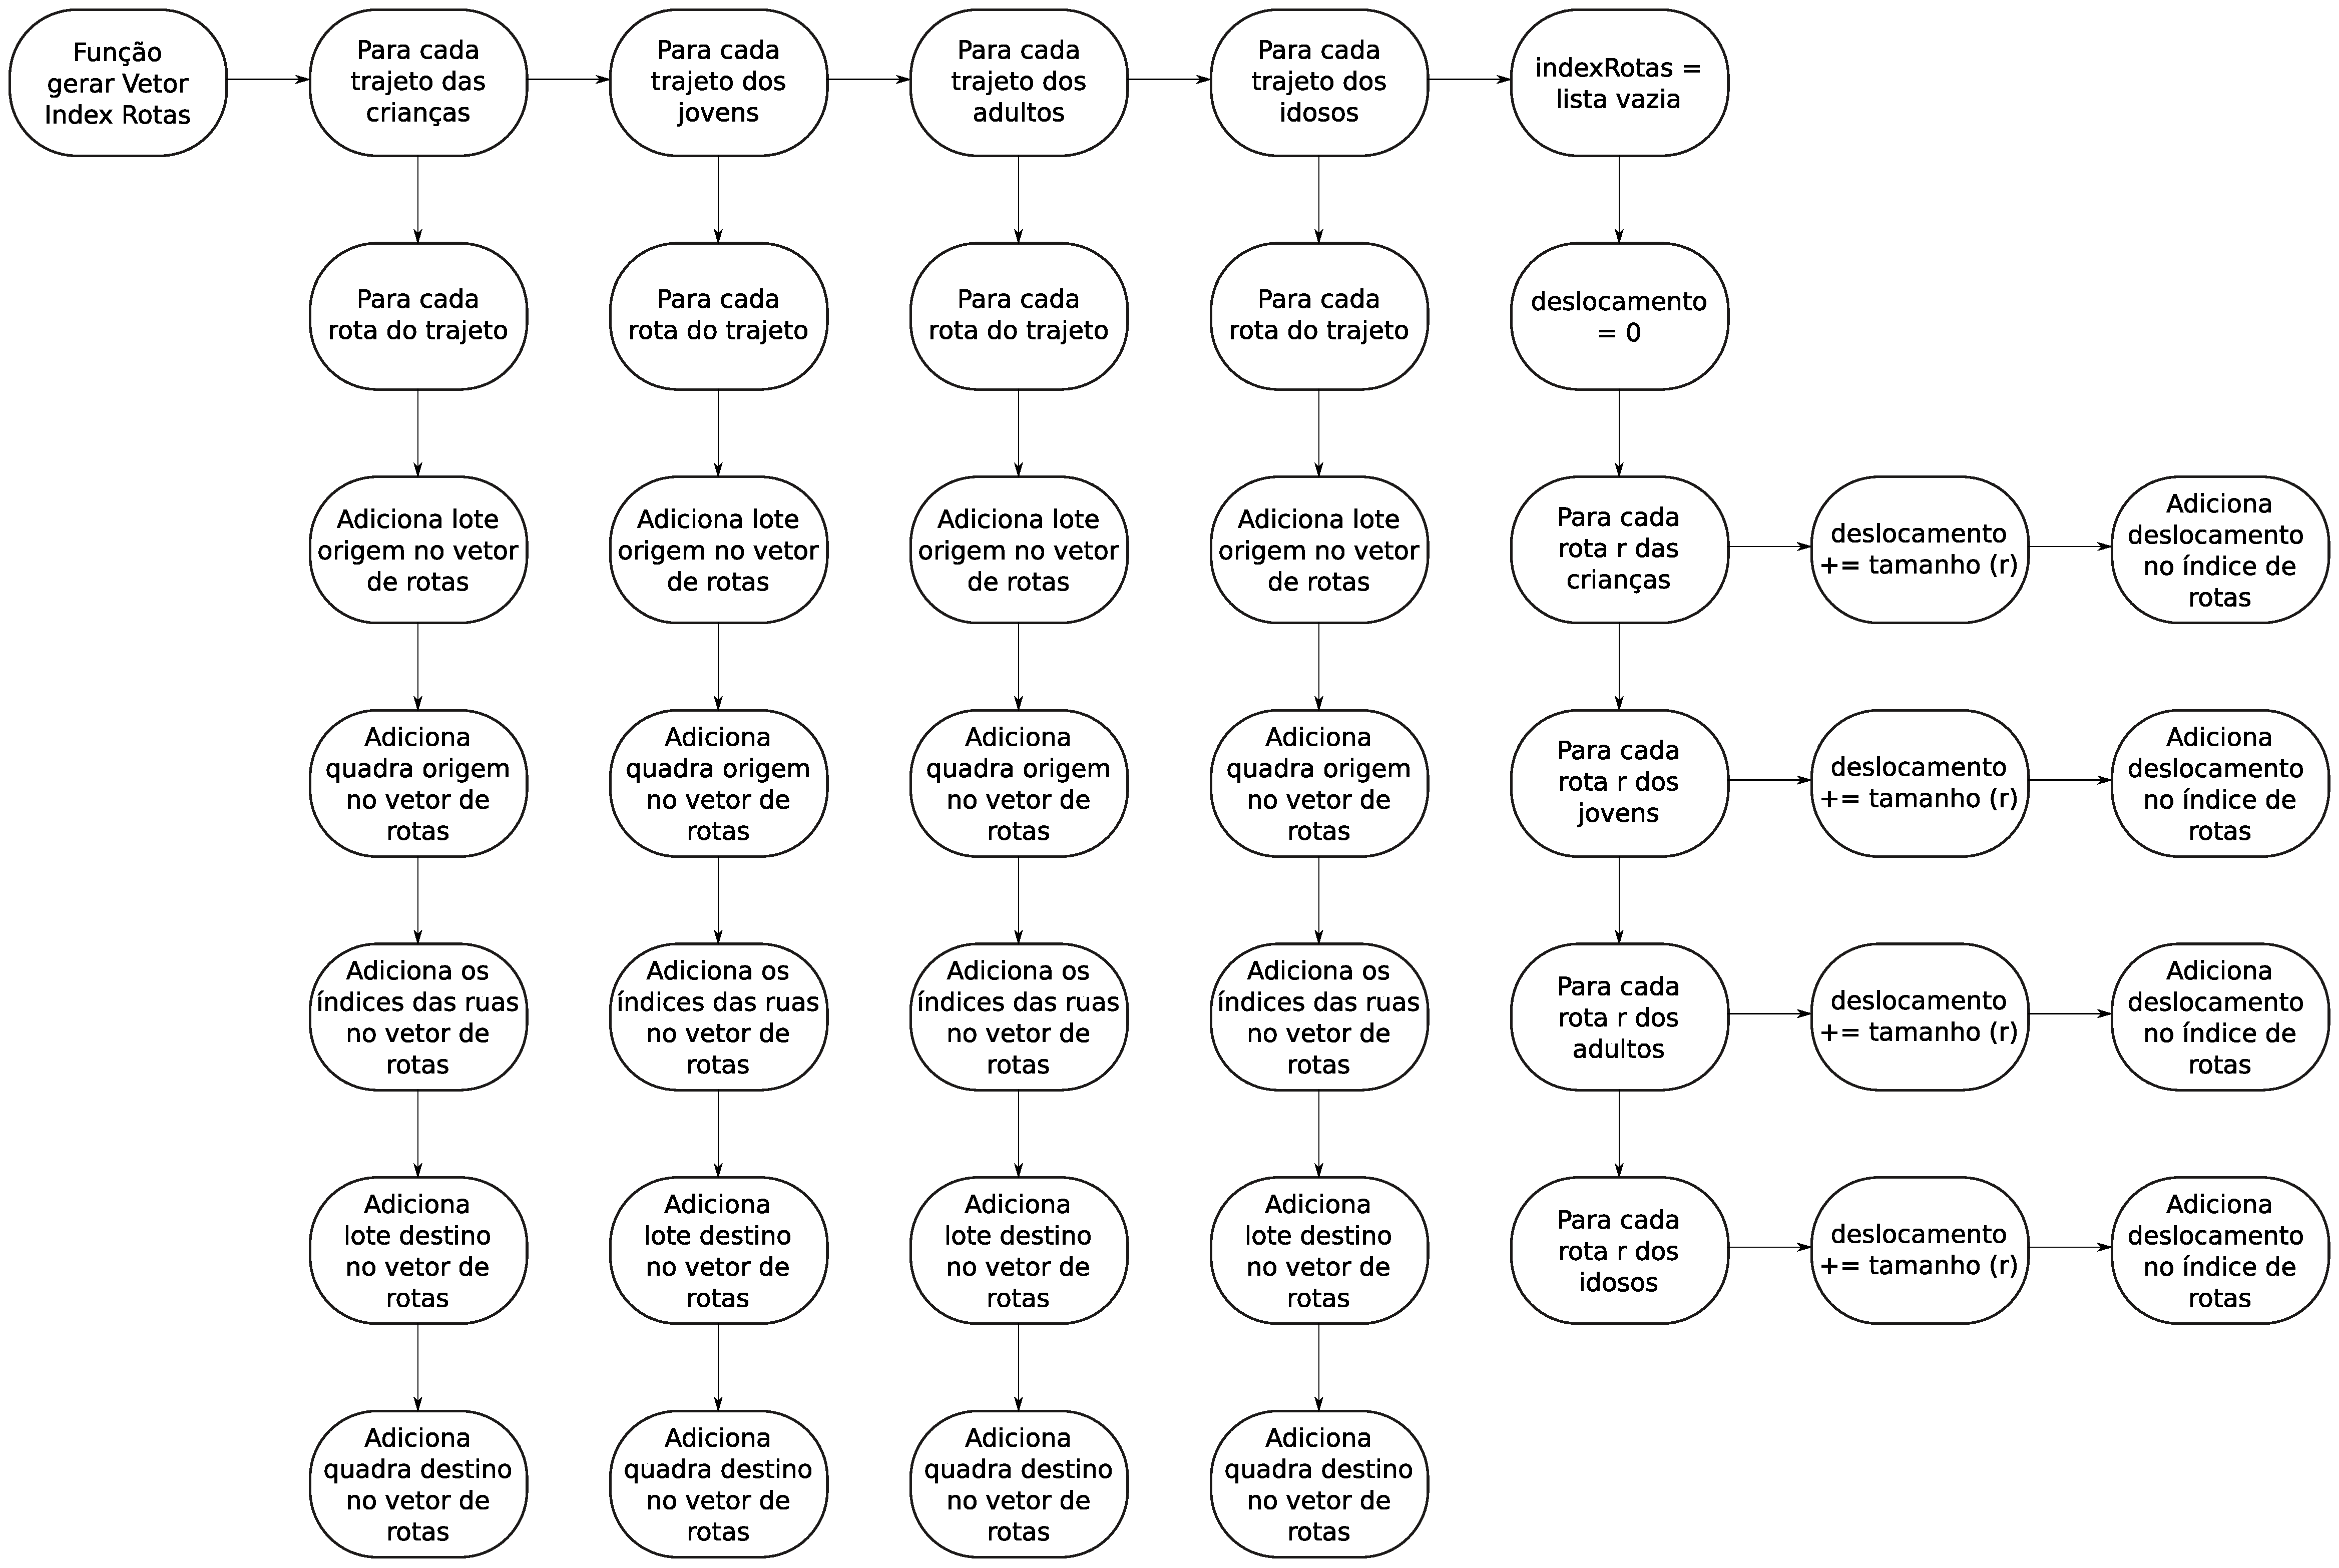
\includegraphics[width=1\textwidth]{Figuras/Simula/Fluxos/gerarVetorIndexRotas.eps}
  \caption{Função gerarVetorIndexRotas.}
  \label{fig:gerarVetorIndexRotas}
\end{figure} 

\newpage

\subsubsection{Função gerarVetorIndexTrajetos}

O Código \ref{cod:gerarVetorIndexTrajetos}, Algoritmo \ref{alg:gerarVetorIndexTrajetos} e Figura \ref{fig:gerarVetorIndexTrajetos} ilustram a rotina responsável pela geração dos índices e do vetor dos trajetos. Os trajetos são utilizados principalmente nas rotinas de movimentação livre e em trajetos dos agentes, mas também são empregados na inicialização da população. Um trajeto é constituído basicamente por um conjunto de rotas. Desta forma, cada trajeto armazena uma lista com os identificadores de suas rotas. Os trajetos são definidos de acordo com as faixas etárias dos agentes. Os índices especificam as posições de início e término de cada trajeto. 

\lstinputlisting[caption=Função gerarVetorIndexTrajetos, label=cod:gerarVetorIndexTrajetos, captionpos=b, language=Java]{Codigos/Simula/Fontes/gerarVetorIndexTrajetos.java}

\begin{algorithm}[H]
   \SetAlgoLined   
   \input{Codigos/Simula/Algoritmos/gerarVetorIndexTrajetos.txt}
   \caption{\textsc{Função gerarVetorIndexTrajetos.}}
   \label{alg:gerarVetorIndexTrajetos}
\end{algorithm}

\begin{figure}[H]
  \centering
  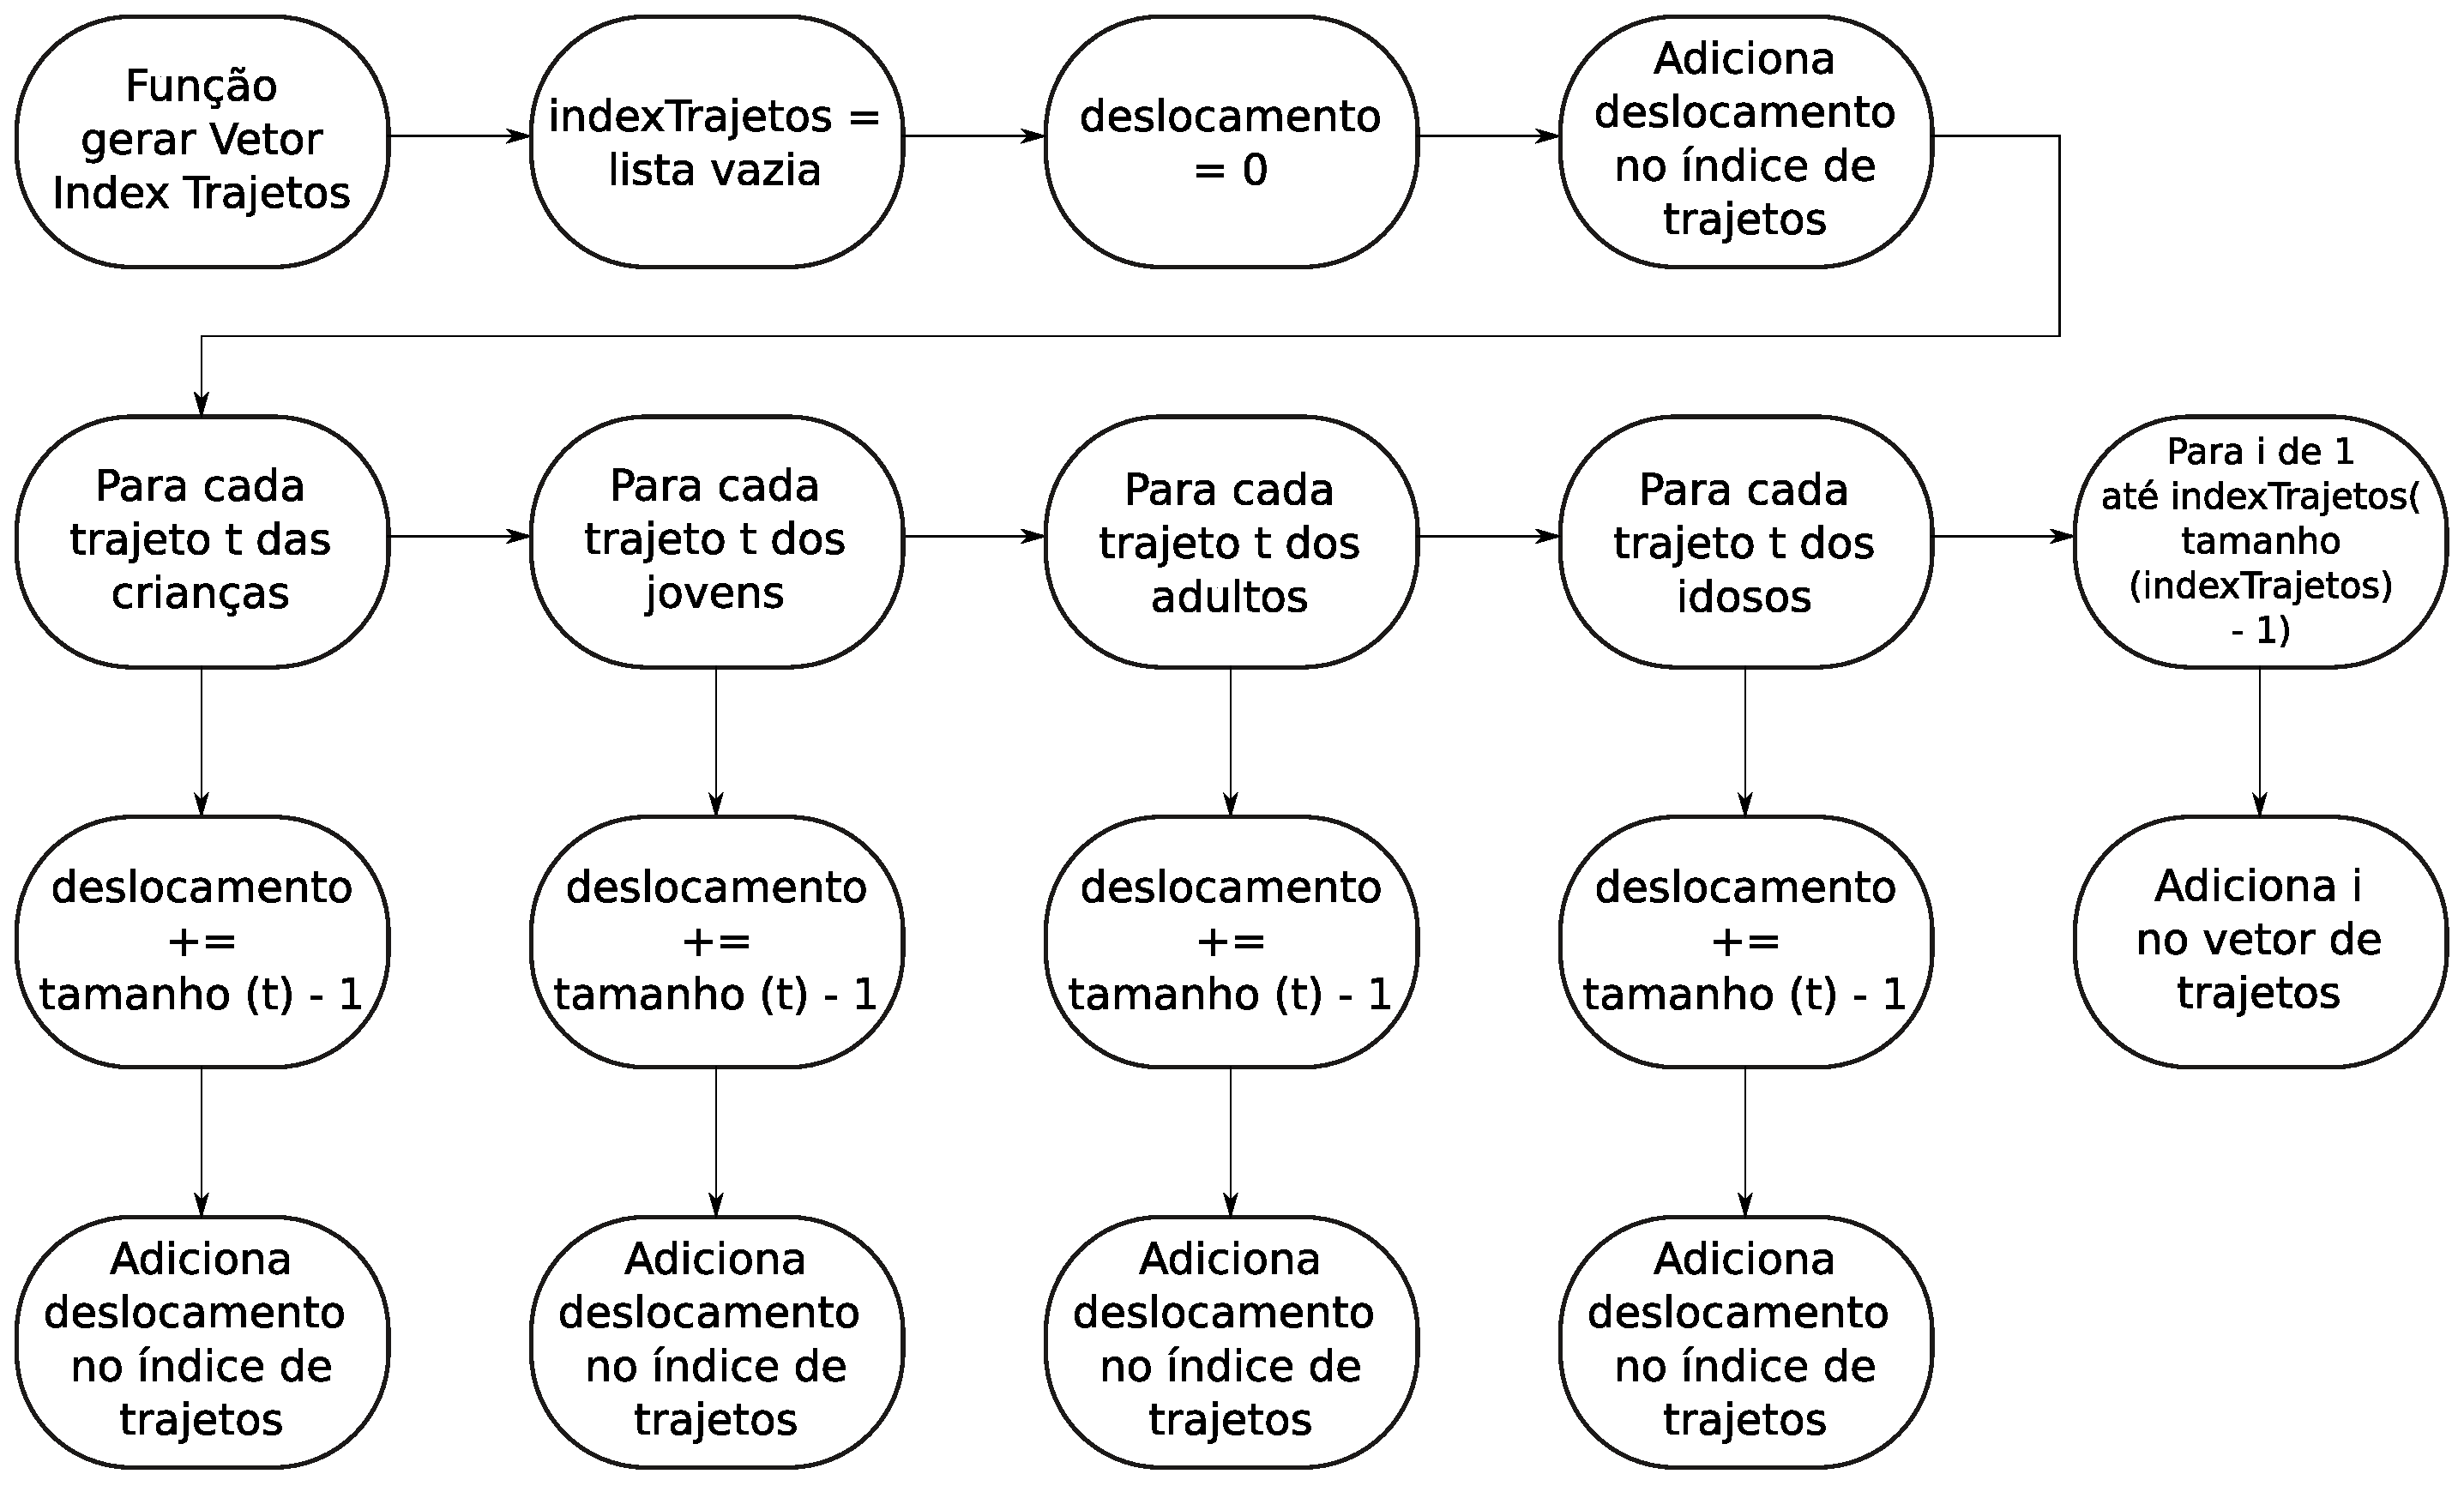
\includegraphics[width=0.9\textwidth]{Figuras/Simula/Fluxos/gerarVetorIndexTrajetos.eps}
  \caption{Função gerarVetorIndexTrajetos.}
  \label{fig:gerarVetorIndexTrajetos}
\end{figure} 

\newpage

\subsubsection{Função gerarVetorIndexPeriodos}

O Código \ref{cod:gerarVetorIndexPeriodos}, Algoritmos \ref{alg:gerarVetorIndexPeriodos1} e \ref{alg:gerarVetorIndexPeriodos2} e Figura \ref{fig:gerarVetorIndexPeriodos} ilustram a rotina responsável pela geração dos índices e do vetor dos períodos dos trajetos. Os períodos dos trajetos são utilizados na rotina de movimentação dos agentes e descrevem a quantidade de ciclos de permanência dos agentes nos lotes de destino. Deste modo, quando chegam à um lote destino de uma rota, os agentes permanecem um período de tempo movimentando-se localmente neste lote, para posteriormente continuar sua movimentação utilizando as demais rotas definidas em seu trajeto. Assim como os trajetos, os períodos dos trajetos são definidos e agrupados de acordo com as faixas etárias dos agentes. Os índices são gerados à nível de faixa etária, viabilizando recuperar rapidamente os períodos dos trajetos pertencentes à determinada faixa etária. 

\lstinputlisting[caption=Função gerarVetorIndexPeriodos, label=cod:gerarVetorIndexPeriodos, captionpos=b, language=Java]{Codigos/Simula/Fontes/gerarVetorIndexPeriodos.java}

\begin{algorithm}[H]
   \SetAlgoLined   
   \input{Codigos/Simula/Algoritmos/gerarVetorIndexPeriodos1.txt}
   \caption{\textsc{Função gerarVetorIndexPeriodos - Parte I.}}
   \label{alg:gerarVetorIndexPeriodos1}
\end{algorithm}

\newpage

\begin{algorithm}[H]
   \SetAlgoLined   
   \input{Codigos/Simula/Algoritmos/gerarVetorIndexPeriodos2.txt}
   \caption{\textsc{Função gerarVetorIndexPeriodos - Parte II.}}
   \label{alg:gerarVetorIndexPeriodos2}
\end{algorithm}

\begin{figure}[H]
  \centering
  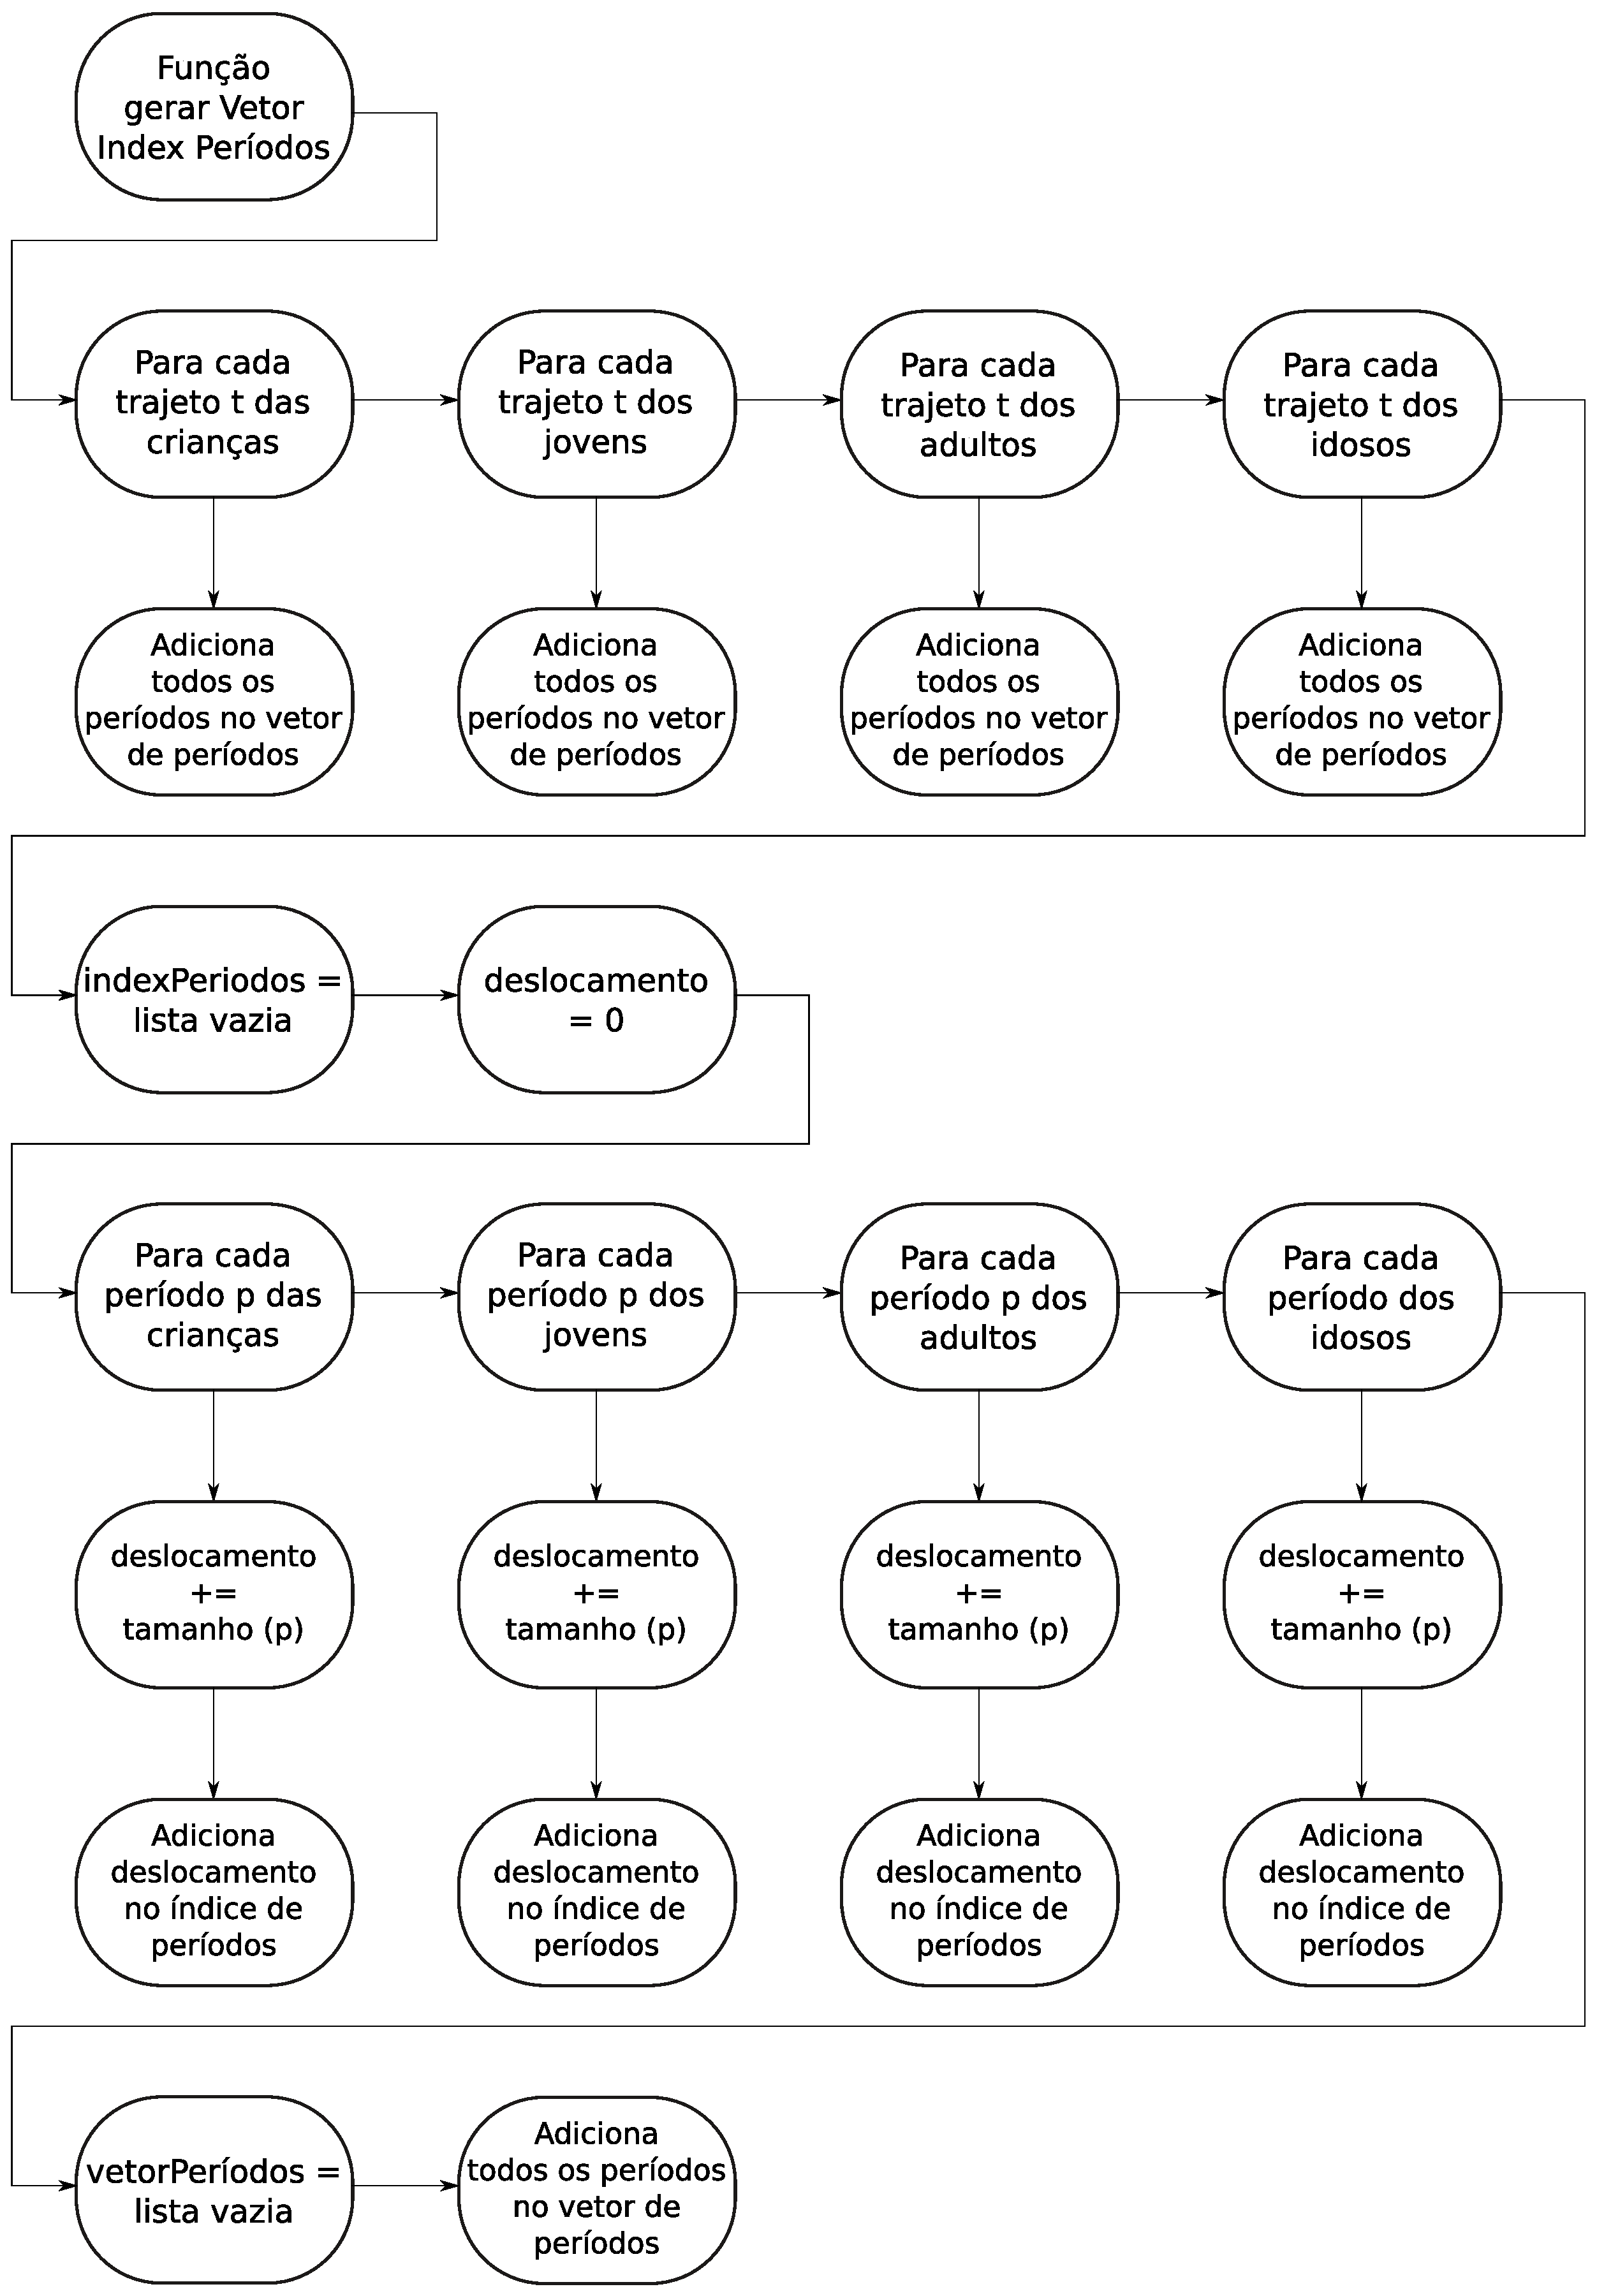
\includegraphics[width=0.7\textwidth]{Figuras/Simula/Fluxos/gerarVetorIndexPeriodos.eps}
  \caption{Função gerarVetorIndexPeriodos.}
  \label{fig:gerarVetorIndexPeriodos}
\end{figure} 

\newpage

\subsubsection{Função gerarIndexTrajetosFaixaEtaria}

O Código \ref{cod:gerarIndexTrajetosFaixaEtaria}, Algoritmo \ref{alg:gerarIndexTrajetosFaixaEtaria} e Figura \ref{fig:gerarIndexTrajetosFaixaEtaria} ilustram a rotina responsável pela geração dos índices dos trajetos por faixa etária. Este índice é utilizado nos processos de definição dos trajetos e movimentação dos agentes, viabilizando localizar rapidamente todos os trajetos pertencentes à uma determinada faixa etária. 

\lstinputlisting[caption=Função gerarIndexTrajetosFaixaEtaria, label=cod:gerarIndexTrajetosFaixaEtaria, captionpos=b, language=Java]{Codigos/Simula/Fontes/gerarIndexTrajetosFaixaEtaria.java}

\begin{algorithm}[H]
   \SetAlgoLined   
   \input{Codigos/Simula/Algoritmos/gerarIndexTrajetosFaixaEtaria.txt}
   \caption{\textsc{Função gerarIndexTrajetosFaixaEtaria.}}
   \label{alg:gerarIndexTrajetosFaixaEtaria}
\end{algorithm}

\begin{figure}[H]
  \centering
  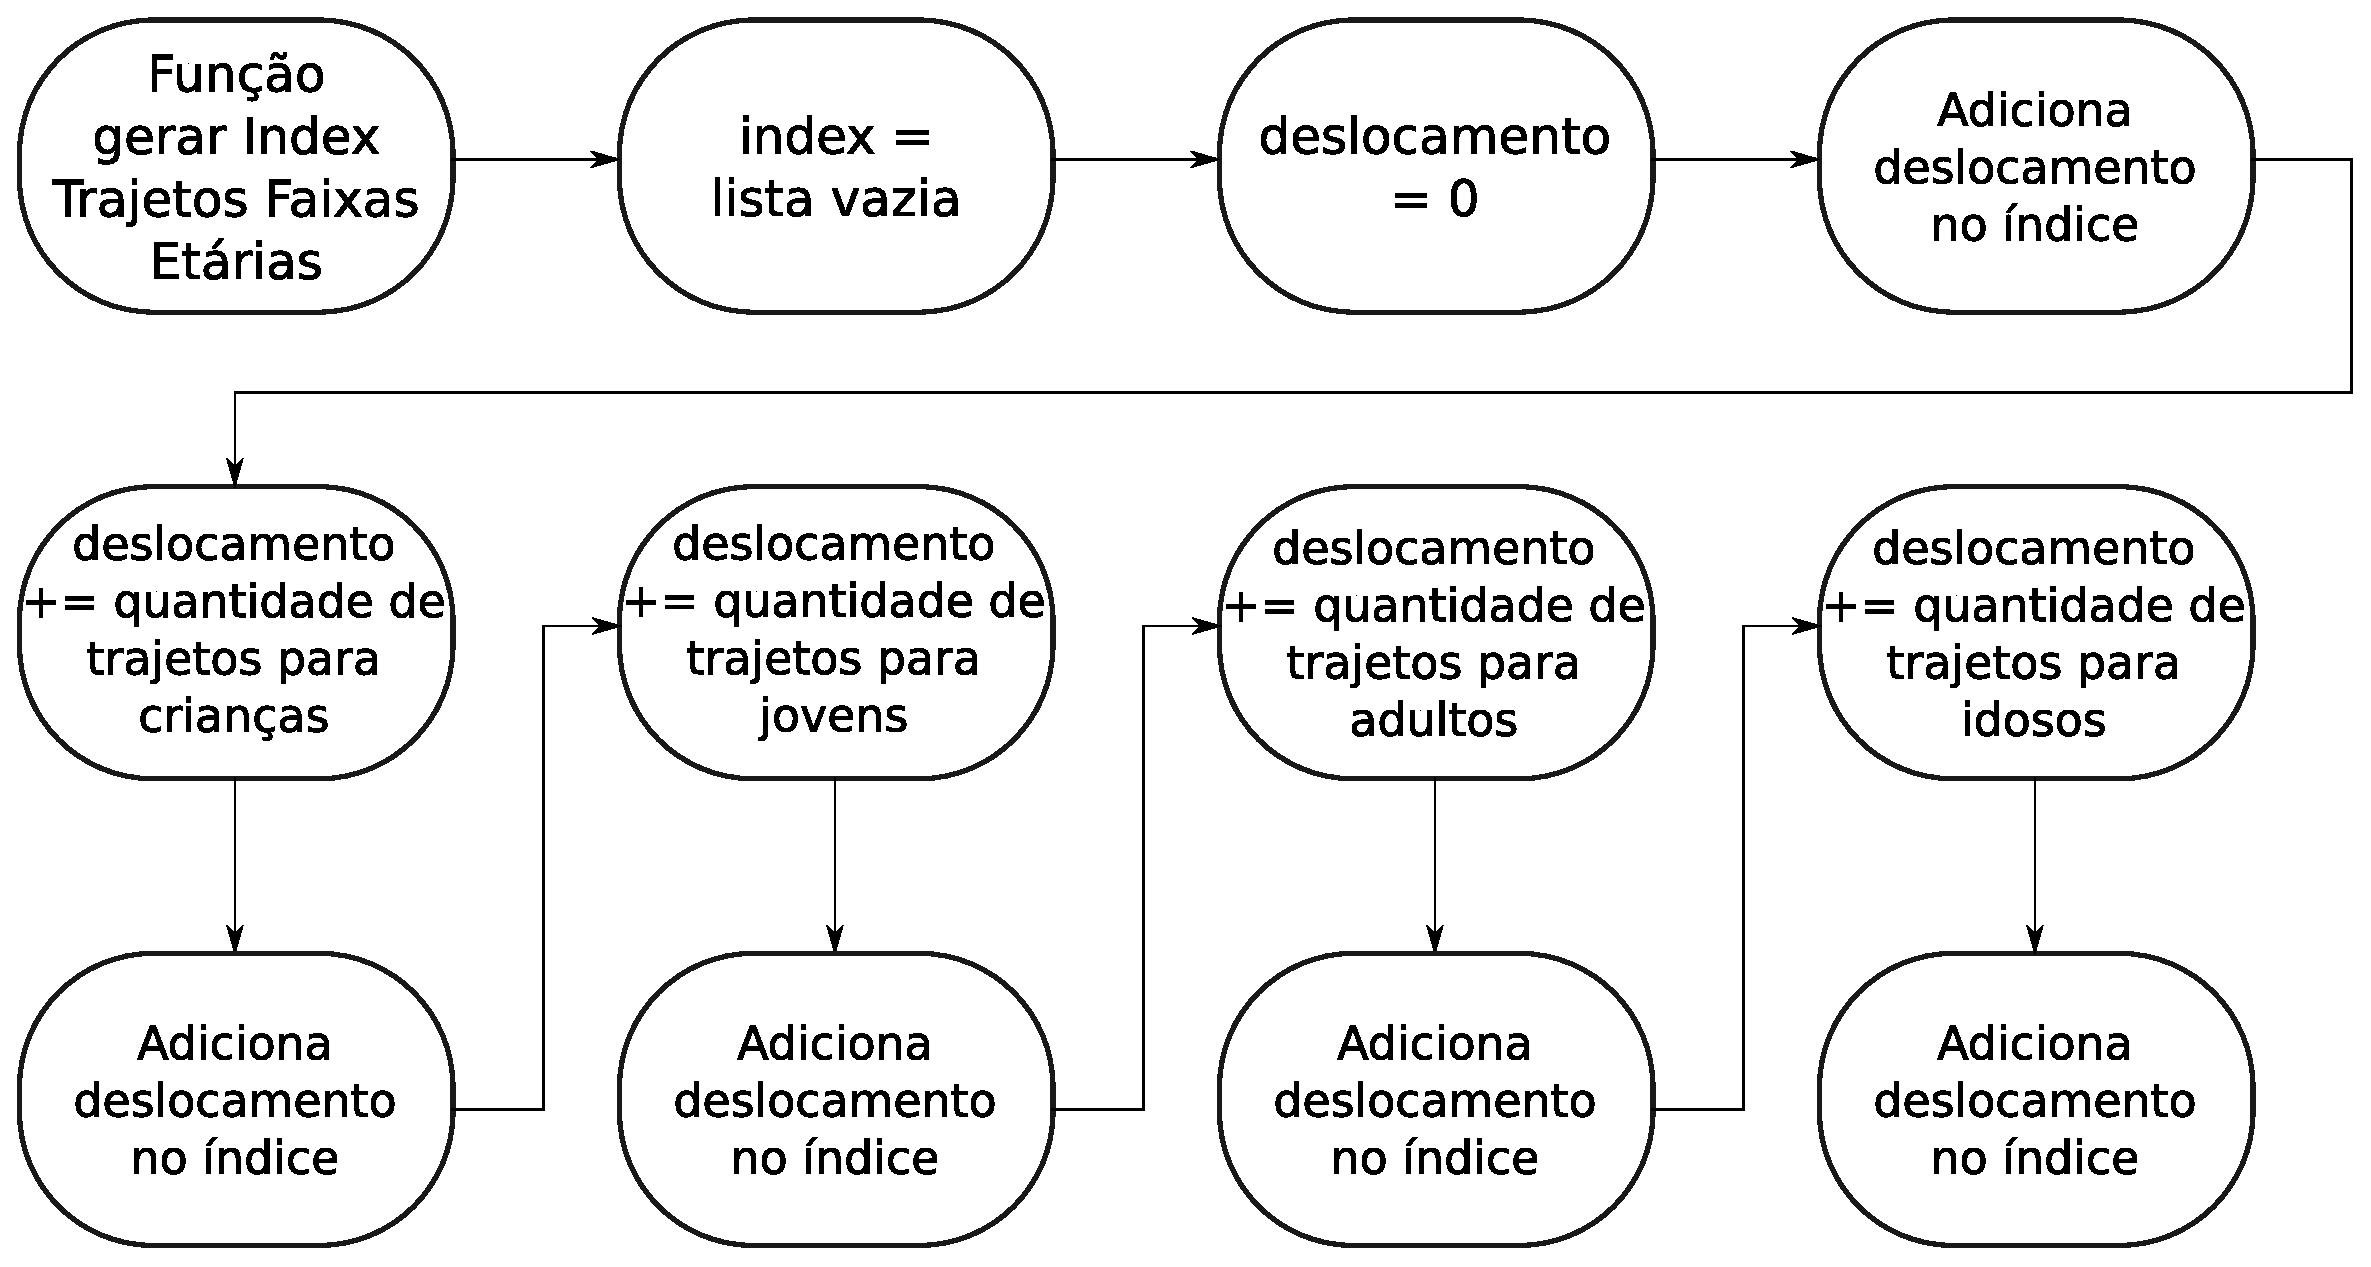
\includegraphics[width=0.8\textwidth]{Figuras/Simula/Fluxos/gerarIndexTrajetosFaixaEtaria.eps}
  \caption{Função gerarIndexTrajetosFaixaEtaria.}
  \label{fig:gerarIndexTrajetosFaixaEtaria}
\end{figure} 

\newpage

\subsubsection{Função escreverArquivoVetores}

O Código \ref{cod:escreverArquivoVetores}, Algoritmos \ref{alg:escreverArquivoVetores1}, \ref{alg:escreverArquivoVetores2} e \ref{alg:escreverArquivoVetores3} e Figura \ref{fig:escreverArquivoVetores} ilustram a rotina responsável pela escrita dos arquivos finais contendo todas as informações relacionadas ao ambiente e à movimentação de agentes. As informações ambientais são escritas no arquivo denominado \textit{"0-AMB.csv"} e as informações relativas à movimentação dos agentes no arquivo \textit{"1-MOV.csv"}.

\lstinputlisting[caption=Função escreverArquivoVetores, label=cod:escreverArquivoVetores, captionpos=b, language=Java]{Codigos/Simula/Fontes/escreverArquivoVetores.java}

\newpage

\begin{algorithm}[H]
   \SetAlgoLined   
   \input{Codigos/Simula/Algoritmos/escreverArquivoVetores1.txt}
   \caption{\textsc{Função escreverArquivoVetores - Parte I.}}
   \label{alg:escreverArquivoVetores1}
\end{algorithm}

\newpage

\begin{algorithm}[H]
   \SetAlgoLined   
   \input{Codigos/Simula/Algoritmos/escreverArquivoVetores2.txt}
   \caption{\textsc{Função escreverArquivoVetores - Parte II.}}
   \label{alg:escreverArquivoVetores2}
\end{algorithm}

\newpage 

\begin{algorithm}[H]
   \SetAlgoLined   
   \input{Codigos/Simula/Algoritmos/escreverArquivoVetores3.txt}
   \caption{\textsc{Função escreverArquivoVetores - Parte III.}}
   \label{alg:escreverArquivoVetores3}
\end{algorithm}

\begin{figure}[H]
  \centering
  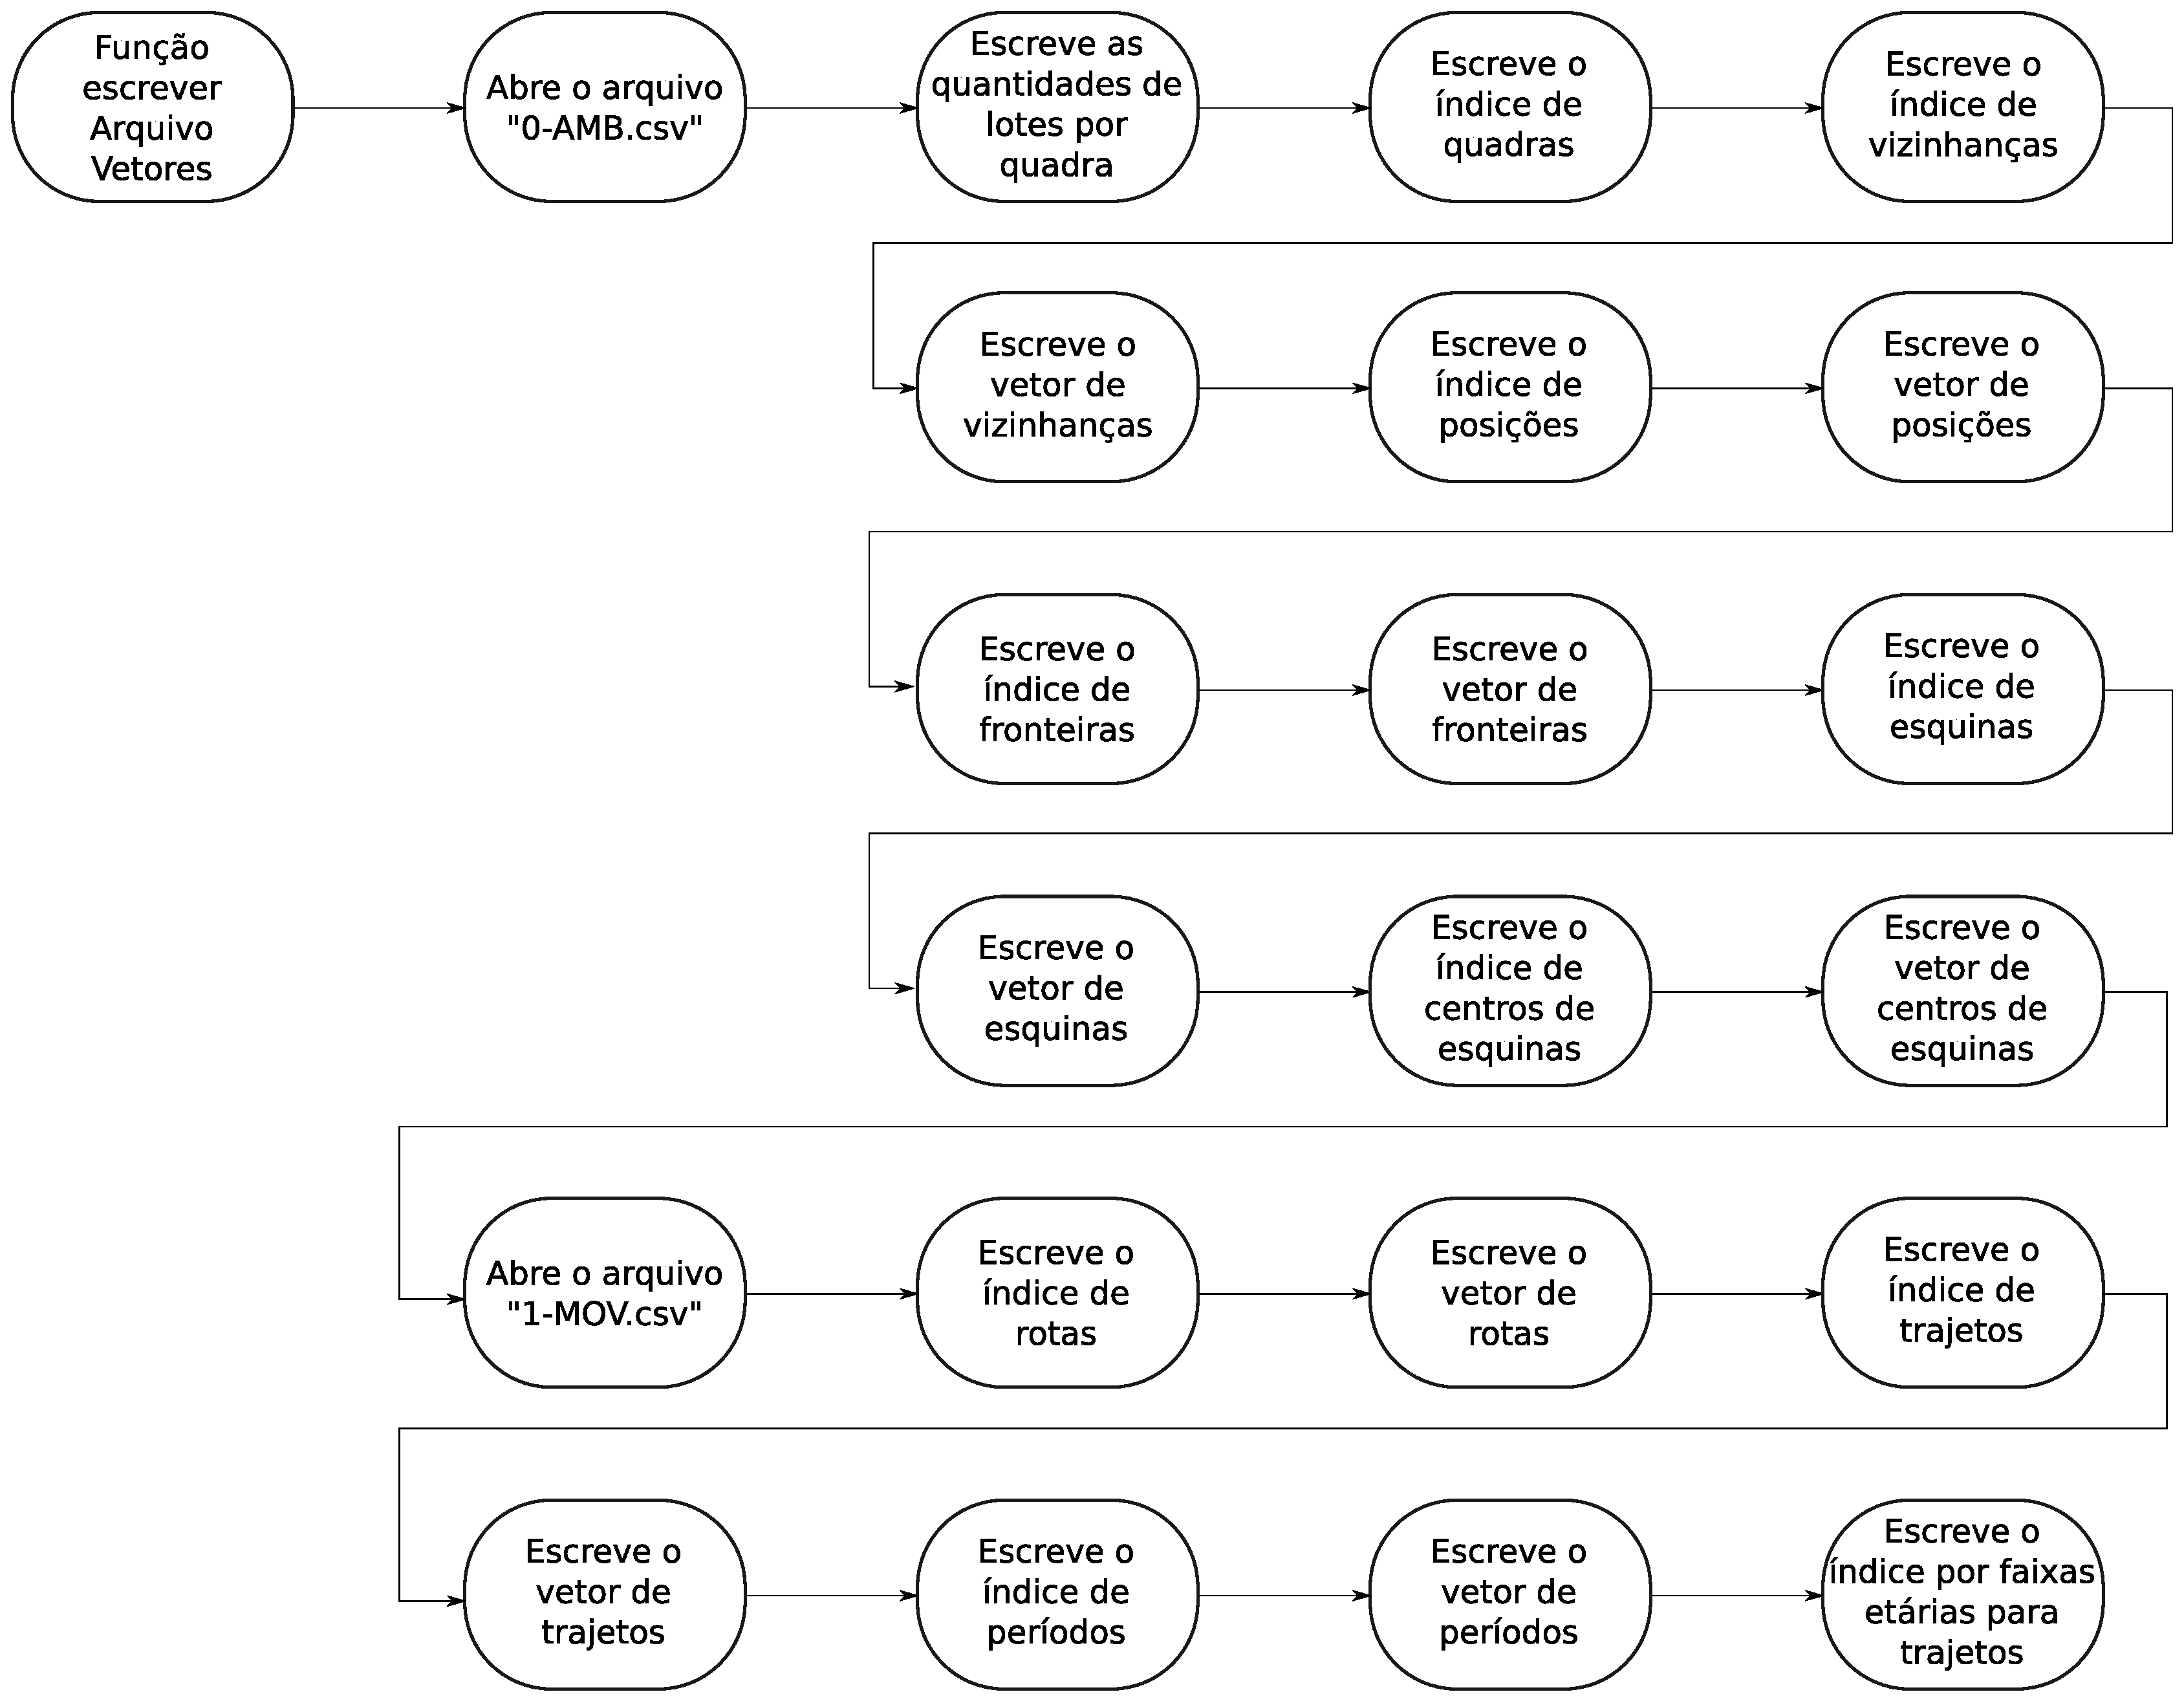
\includegraphics[width=1\textwidth]{Figuras/Simula/Fluxos/escreverArquivoVetores.eps}
  \caption{Função escreverArquivoVetores.}
  \label{fig:escreverArquivoVetores}
\end{figure} 

\newpage

\subsubsection{Função getRegiao}

O Código \ref{cod:getRegiao}, Algoritmo \ref{alg:getRegiao} e Figura \ref{fig:getRegiao} ilustram a rotina responsável pela identificação do índice da região que uma quadra pertence. Este índice é utilizado para identificar as quadras que pertencem às ruas das quadras urbanas e rurais.  

\lstinputlisting[caption=Função getRegiao, label=cod:getRegiao, captionpos=b, language=Java]{Codigos/Simula/Fontes/getRegiao.java}

\begin{algorithm}[H]
   \SetAlgoLined   
   \input{Codigos/Simula/Algoritmos/getRegiao.txt}
   \caption{\textsc{Função getRegiao.}}
   \label{alg:getRegiao}
\end{algorithm}

\begin{figure}[H]
  \centering
  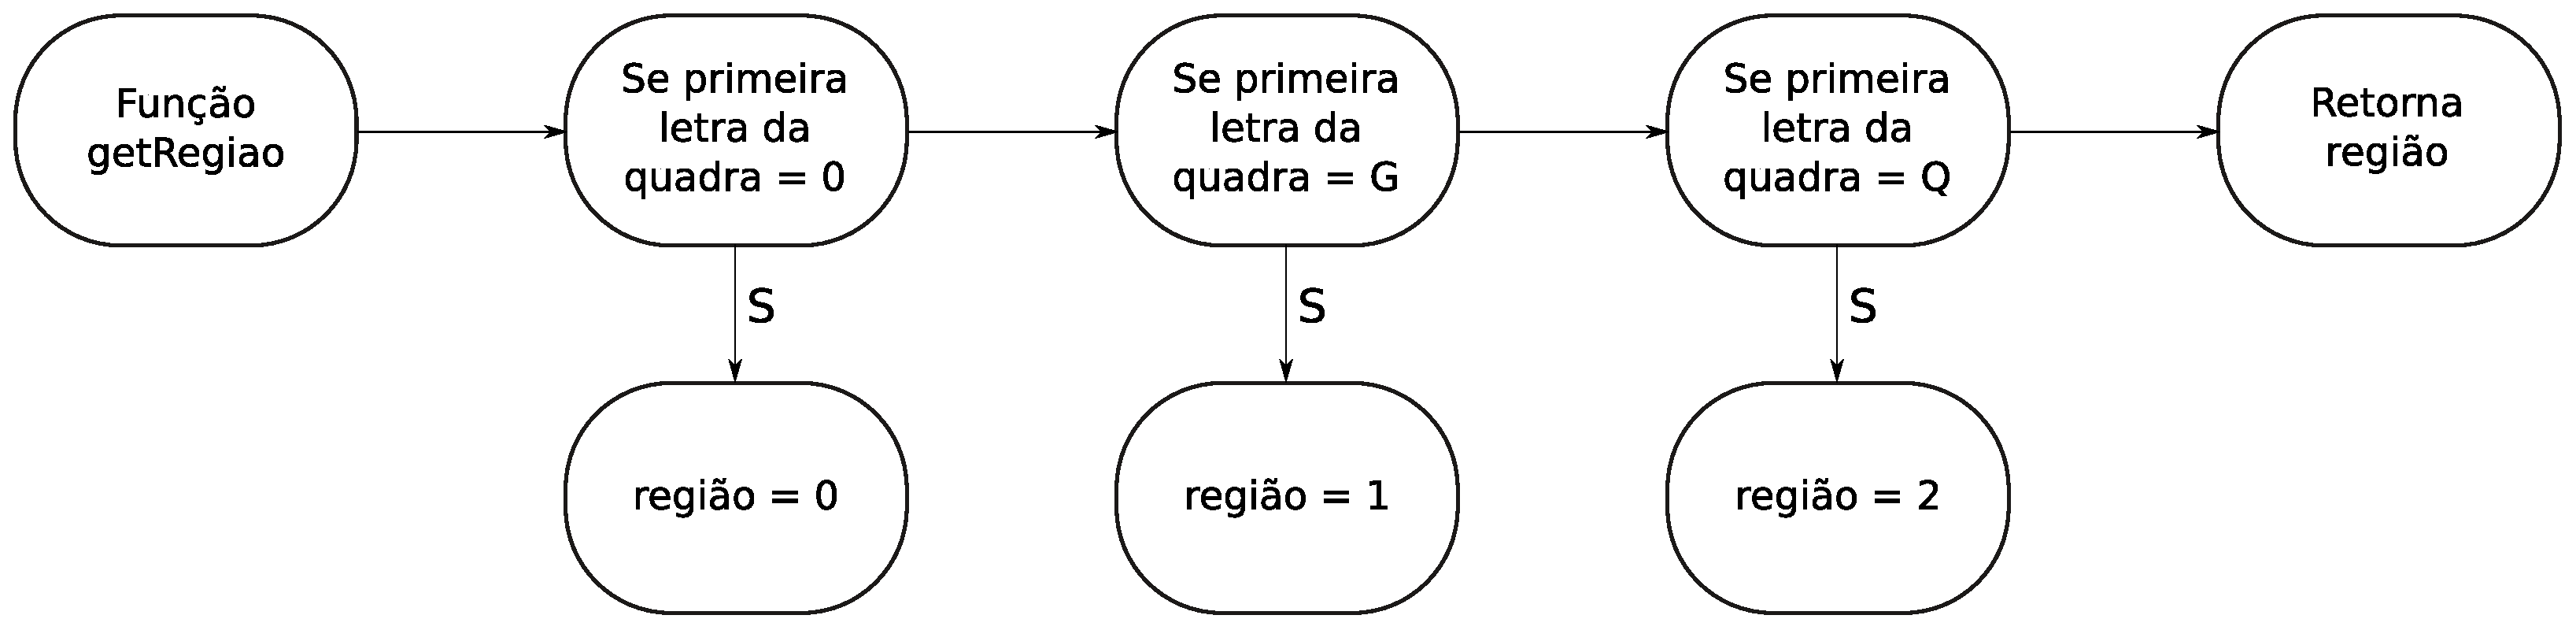
\includegraphics[width=1\textwidth]{Figuras/Simula/Fluxos/getRegiao.eps}
  \caption{Função getRegiao.}
  \label{fig:getRegiao}
\end{figure} 

\newpage

\subsubsection{Função gerarIndexPosicoesRegioes}

O Código \ref{cod:gerarIndexPosicoesRegioes}, Algoritmo \ref{alg:gerarIndexPosicoesRegioes} e Figura \ref{fig:gerarIndexPosicoesRegioes} ilustram a rotina responsável pela geração dos índices das posições por tipo de região. Este índice é utilizado na distribuição dos agentes em posições pertencentes à quadras rurais. 

\lstinputlisting[caption=Função gerarIndexPosicoesRegioes, label=cod:gerarIndexPosicoesRegioes, captionpos=b, language=Java]{Codigos/Simula/Fontes/gerarIndexPosicoesRegioes.java}

\begin{algorithm}[H]
   \SetAlgoLined   
   \input{Codigos/Simula/Algoritmos/gerarIndexPosicoesRegioes.txt}
   \caption{\textsc{Função gerarIndexPosicoesRegioes.}}
   \label{alg:gerarIndexPosicoesRegioes}
\end{algorithm}

\begin{figure}[H]
  \centering
  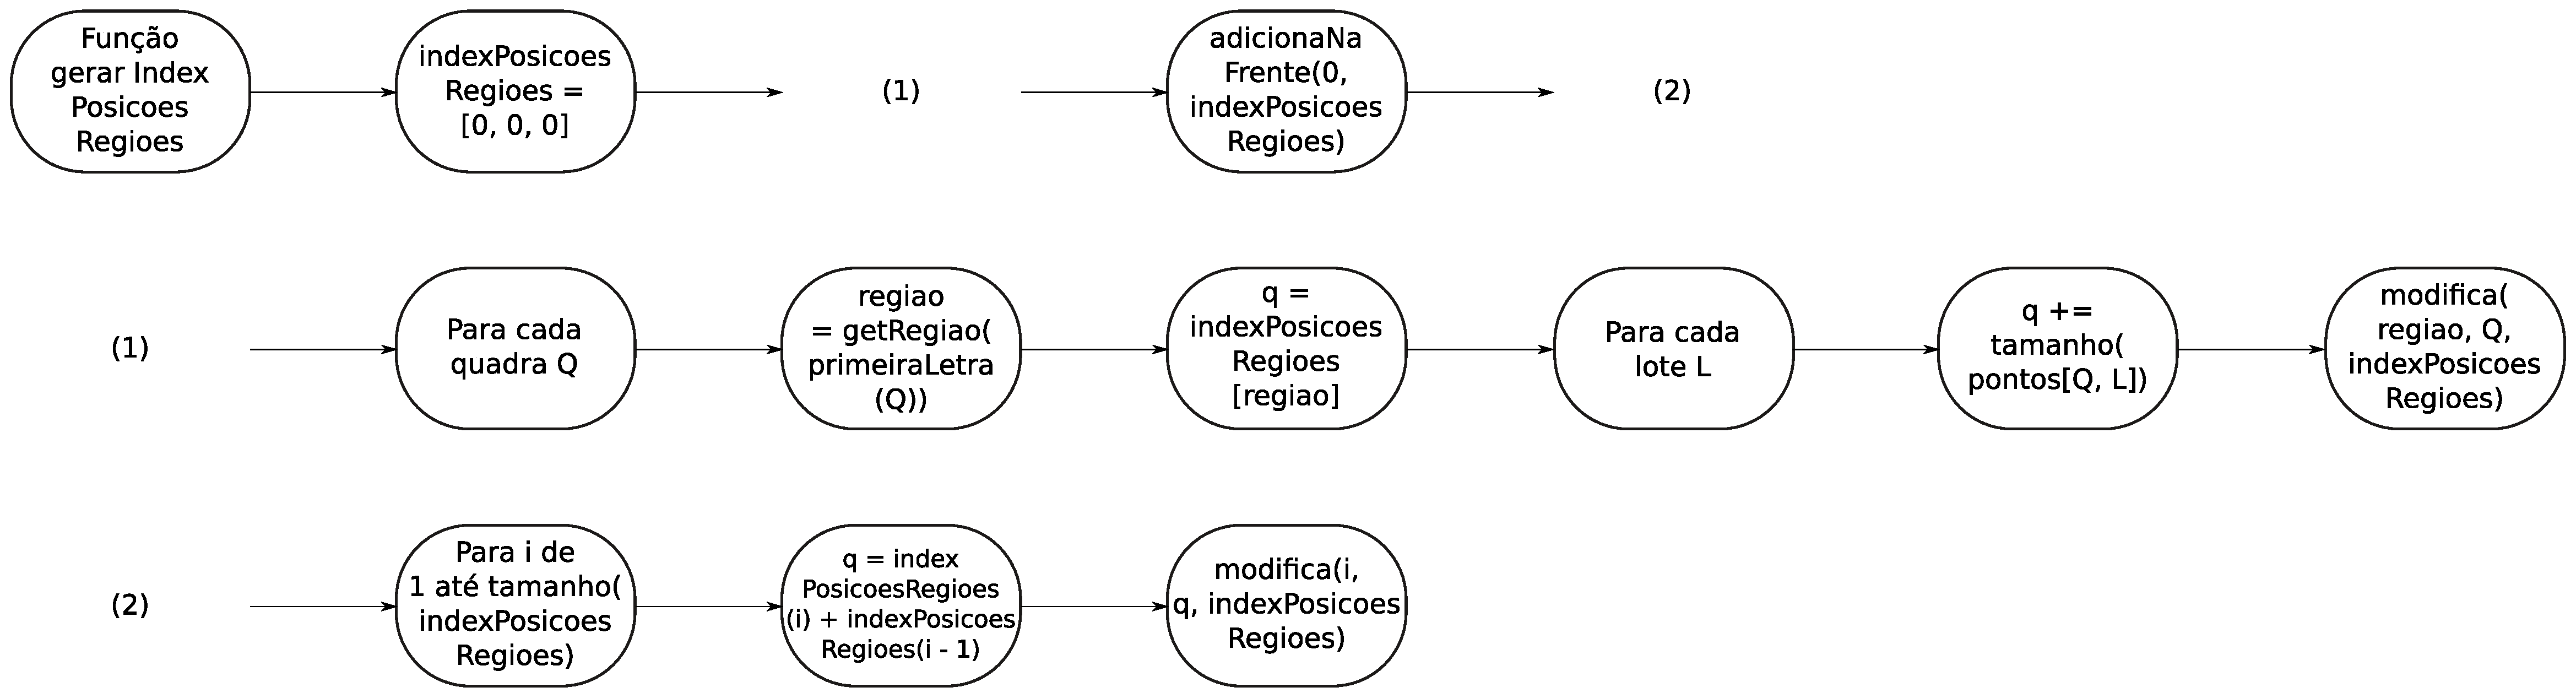
\includegraphics[width=1\textwidth]{Figuras/Simula/Fluxos/gerarIndexPosicoesRegioes.eps}
  \caption{Função gerarIndexPosicoesRegioes.}
  \label{fig:gerarIndexPosicoesRegioes}
\end{figure} 

\newpage

\subsubsection{Função criarDistribuicaoMosquitos}

O Código \ref{cod:criarDistribuicaoMosquitos}, Algoritmo \ref{alg:criarDistribuicaoMosquitos} e Figura \ref{fig:criarDistribuicaoMosquitos} ilustram a rotina responsável pela geração do arquivo de distribuição rural dos agentes. Este arquivo é utilizado no processo de criação das populações iniciais de agentes durante o processo de simulação. A definição das populações de agentes são definidas manualmente no código-fonte. 

\lstinputlisting[caption=Função criarDistribuicaoMosquitos, label=cod:criarDistribuicaoMosquitos, captionpos=b, language=Java]{Codigos/Simula/Fontes/criarDistribuicaoMosquitos.java}

\begin{algorithm}[H]
   \SetAlgoLined   
   \input{Codigos/Simula/Algoritmos/criarDistribuicaoMosquitos.txt}
   \caption{\textsc{Função criarDistribuicaoMosquitos.}}
   \label{alg:criarDistribuicaoMosquitos}
\end{algorithm}

\begin{figure}[H]
  \centering
  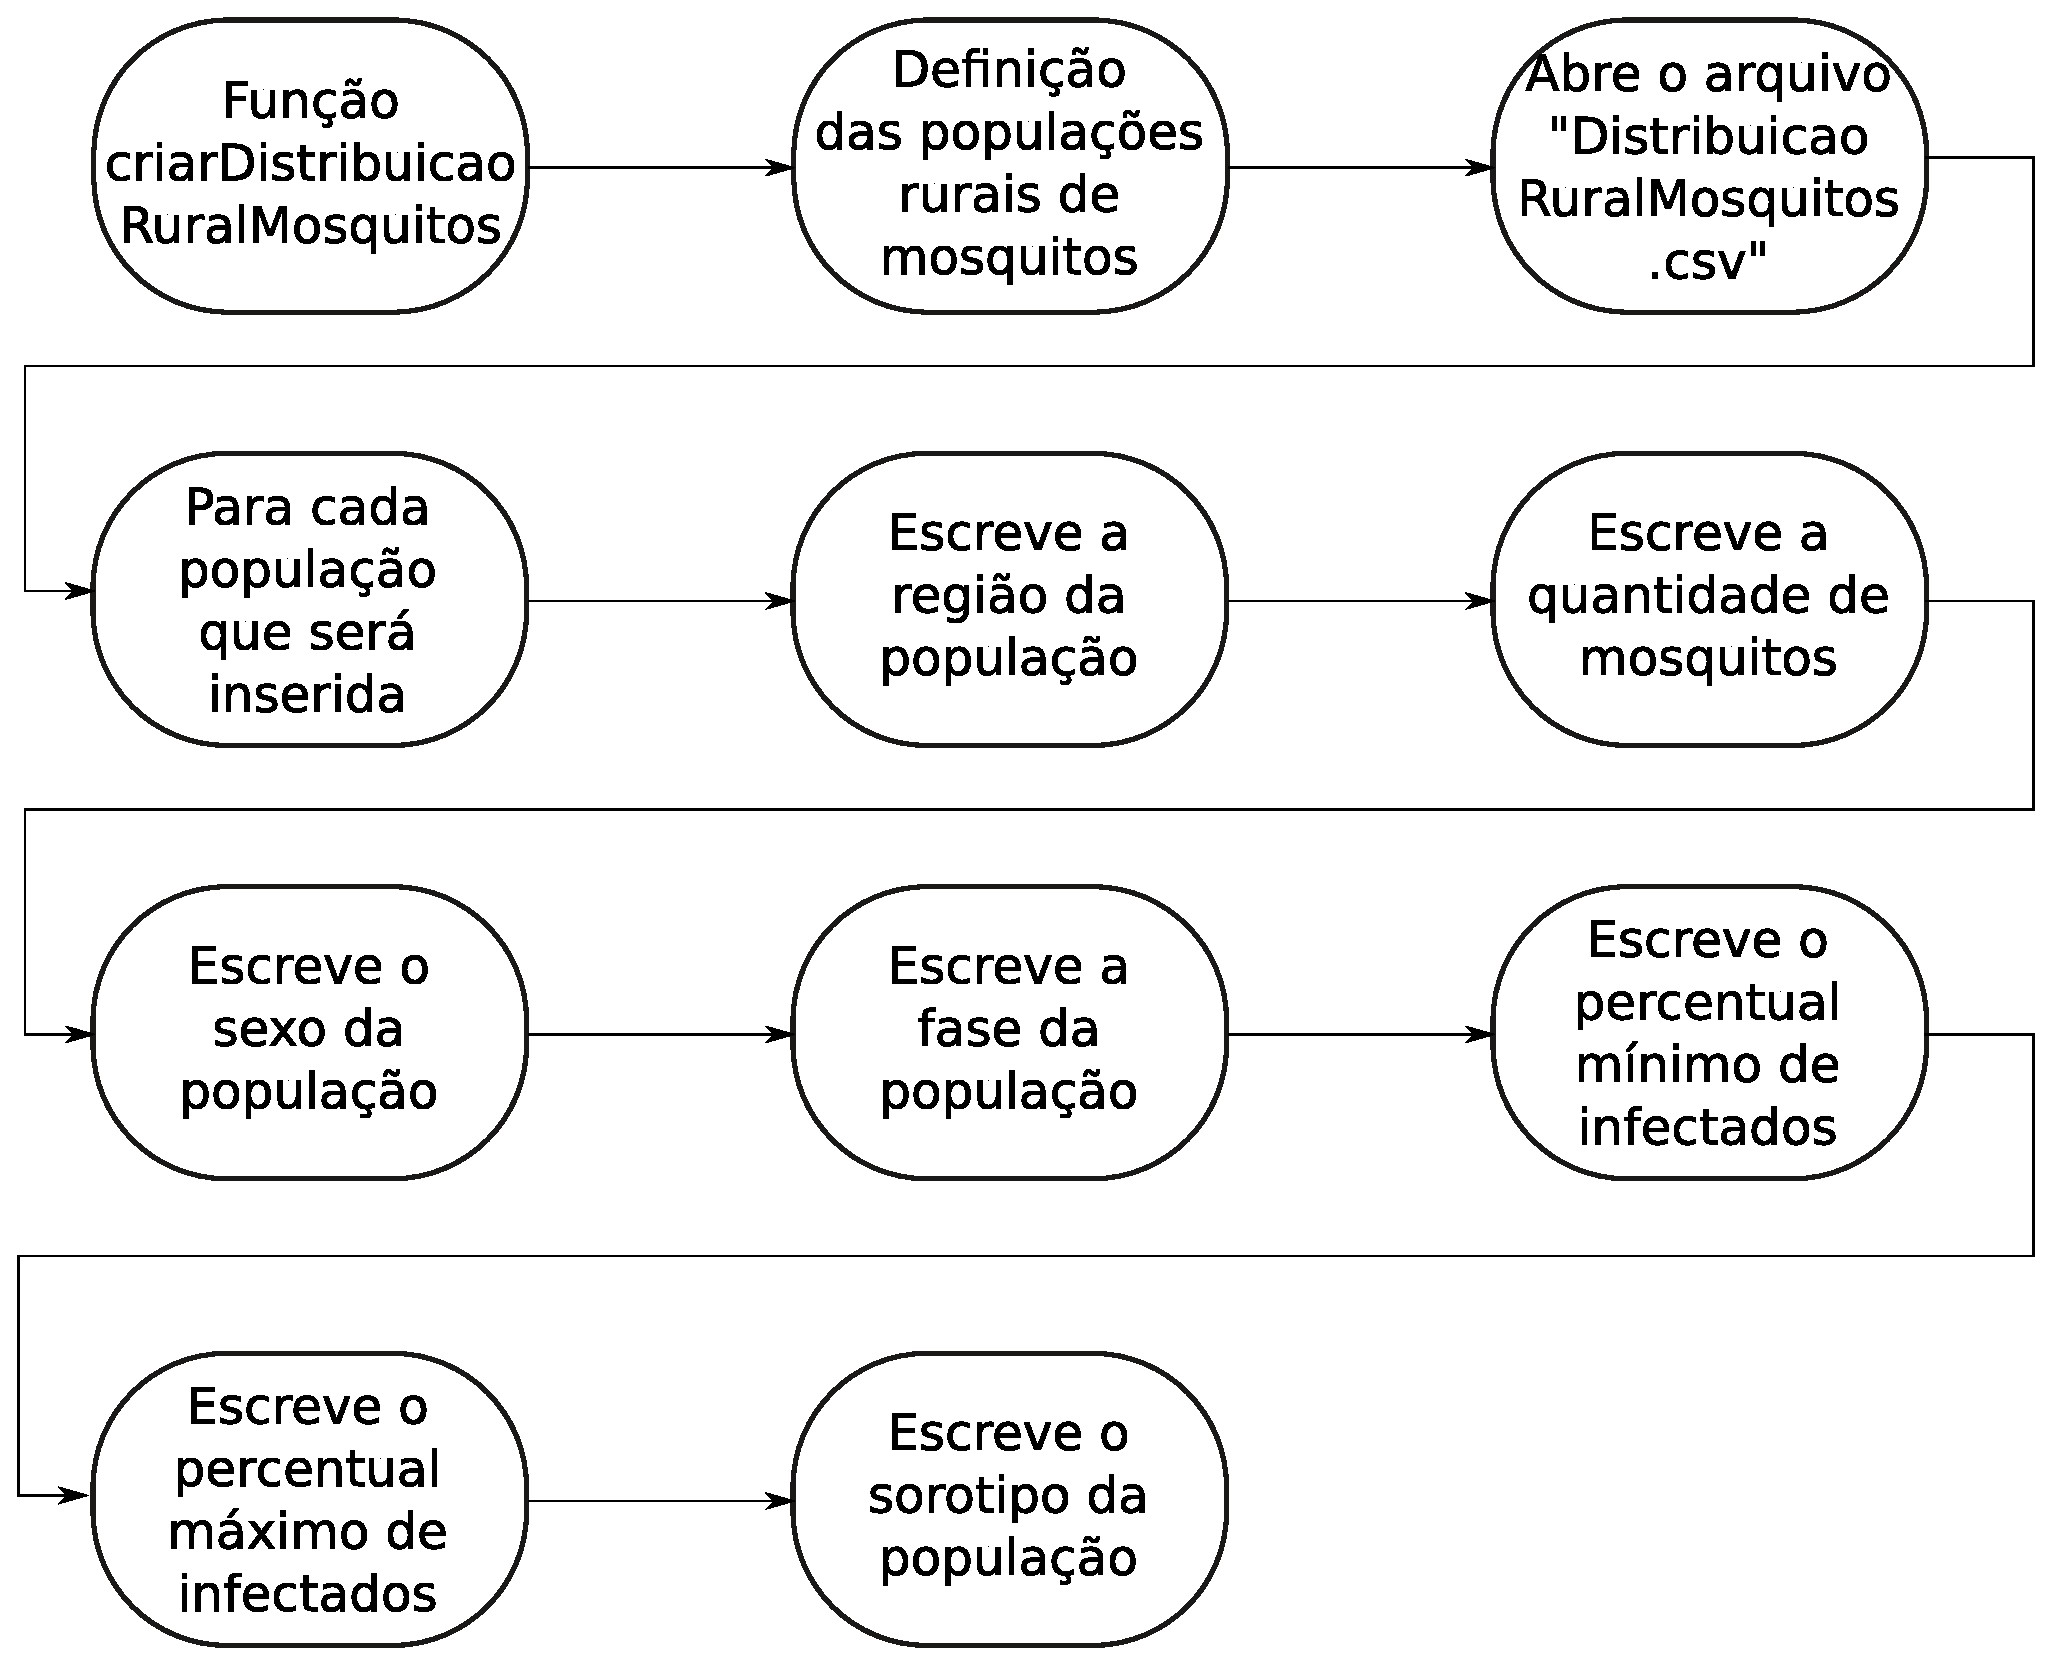
\includegraphics[width=0.6\textwidth]{Figuras/Simula/Fluxos/criarDistribuicaoMosquitos.eps}
  \caption{Função criarDistribuicaoMosquitos.}
  \label{fig:criarDistribuicaoMosquitos}
\end{figure} 

\newpage

\subsubsection{Função criarDistribuicaoHumanos}

O Código \ref{cod:criarDistribuicaoHumanos}, Algoritmo \ref{alg:criarDistribuicaoHumanos} e Figura \ref{fig:criarDistribuicaoHumanos} ilustram a rotina responsável pela geração do arquivo de distribuição rural dos agentes. Este arquivo é utilizado no processo de criação das populações iniciais de agentes durante o processo de simulação. A definição das populações de agentes são definidas manualmente no código-fonte. 

\lstinputlisting[caption=Função criarDistribuicaoHumanos, label=cod:criarDistribuicaoHumanos, captionpos=b, language=Java]{Codigos/Simula/Fontes/criarDistribuicaoHumanos.java}

\begin{algorithm}[H]
   \SetAlgoLined   
   \input{Codigos/Simula/Algoritmos/criarDistribuicaoHumanos.txt}
   \caption{\textsc{Função criarDistribuicaoHumanos.}}
   \label{alg:criarDistribuicaoHumanos}
\end{algorithm}

\begin{figure}[H]
  \centering
  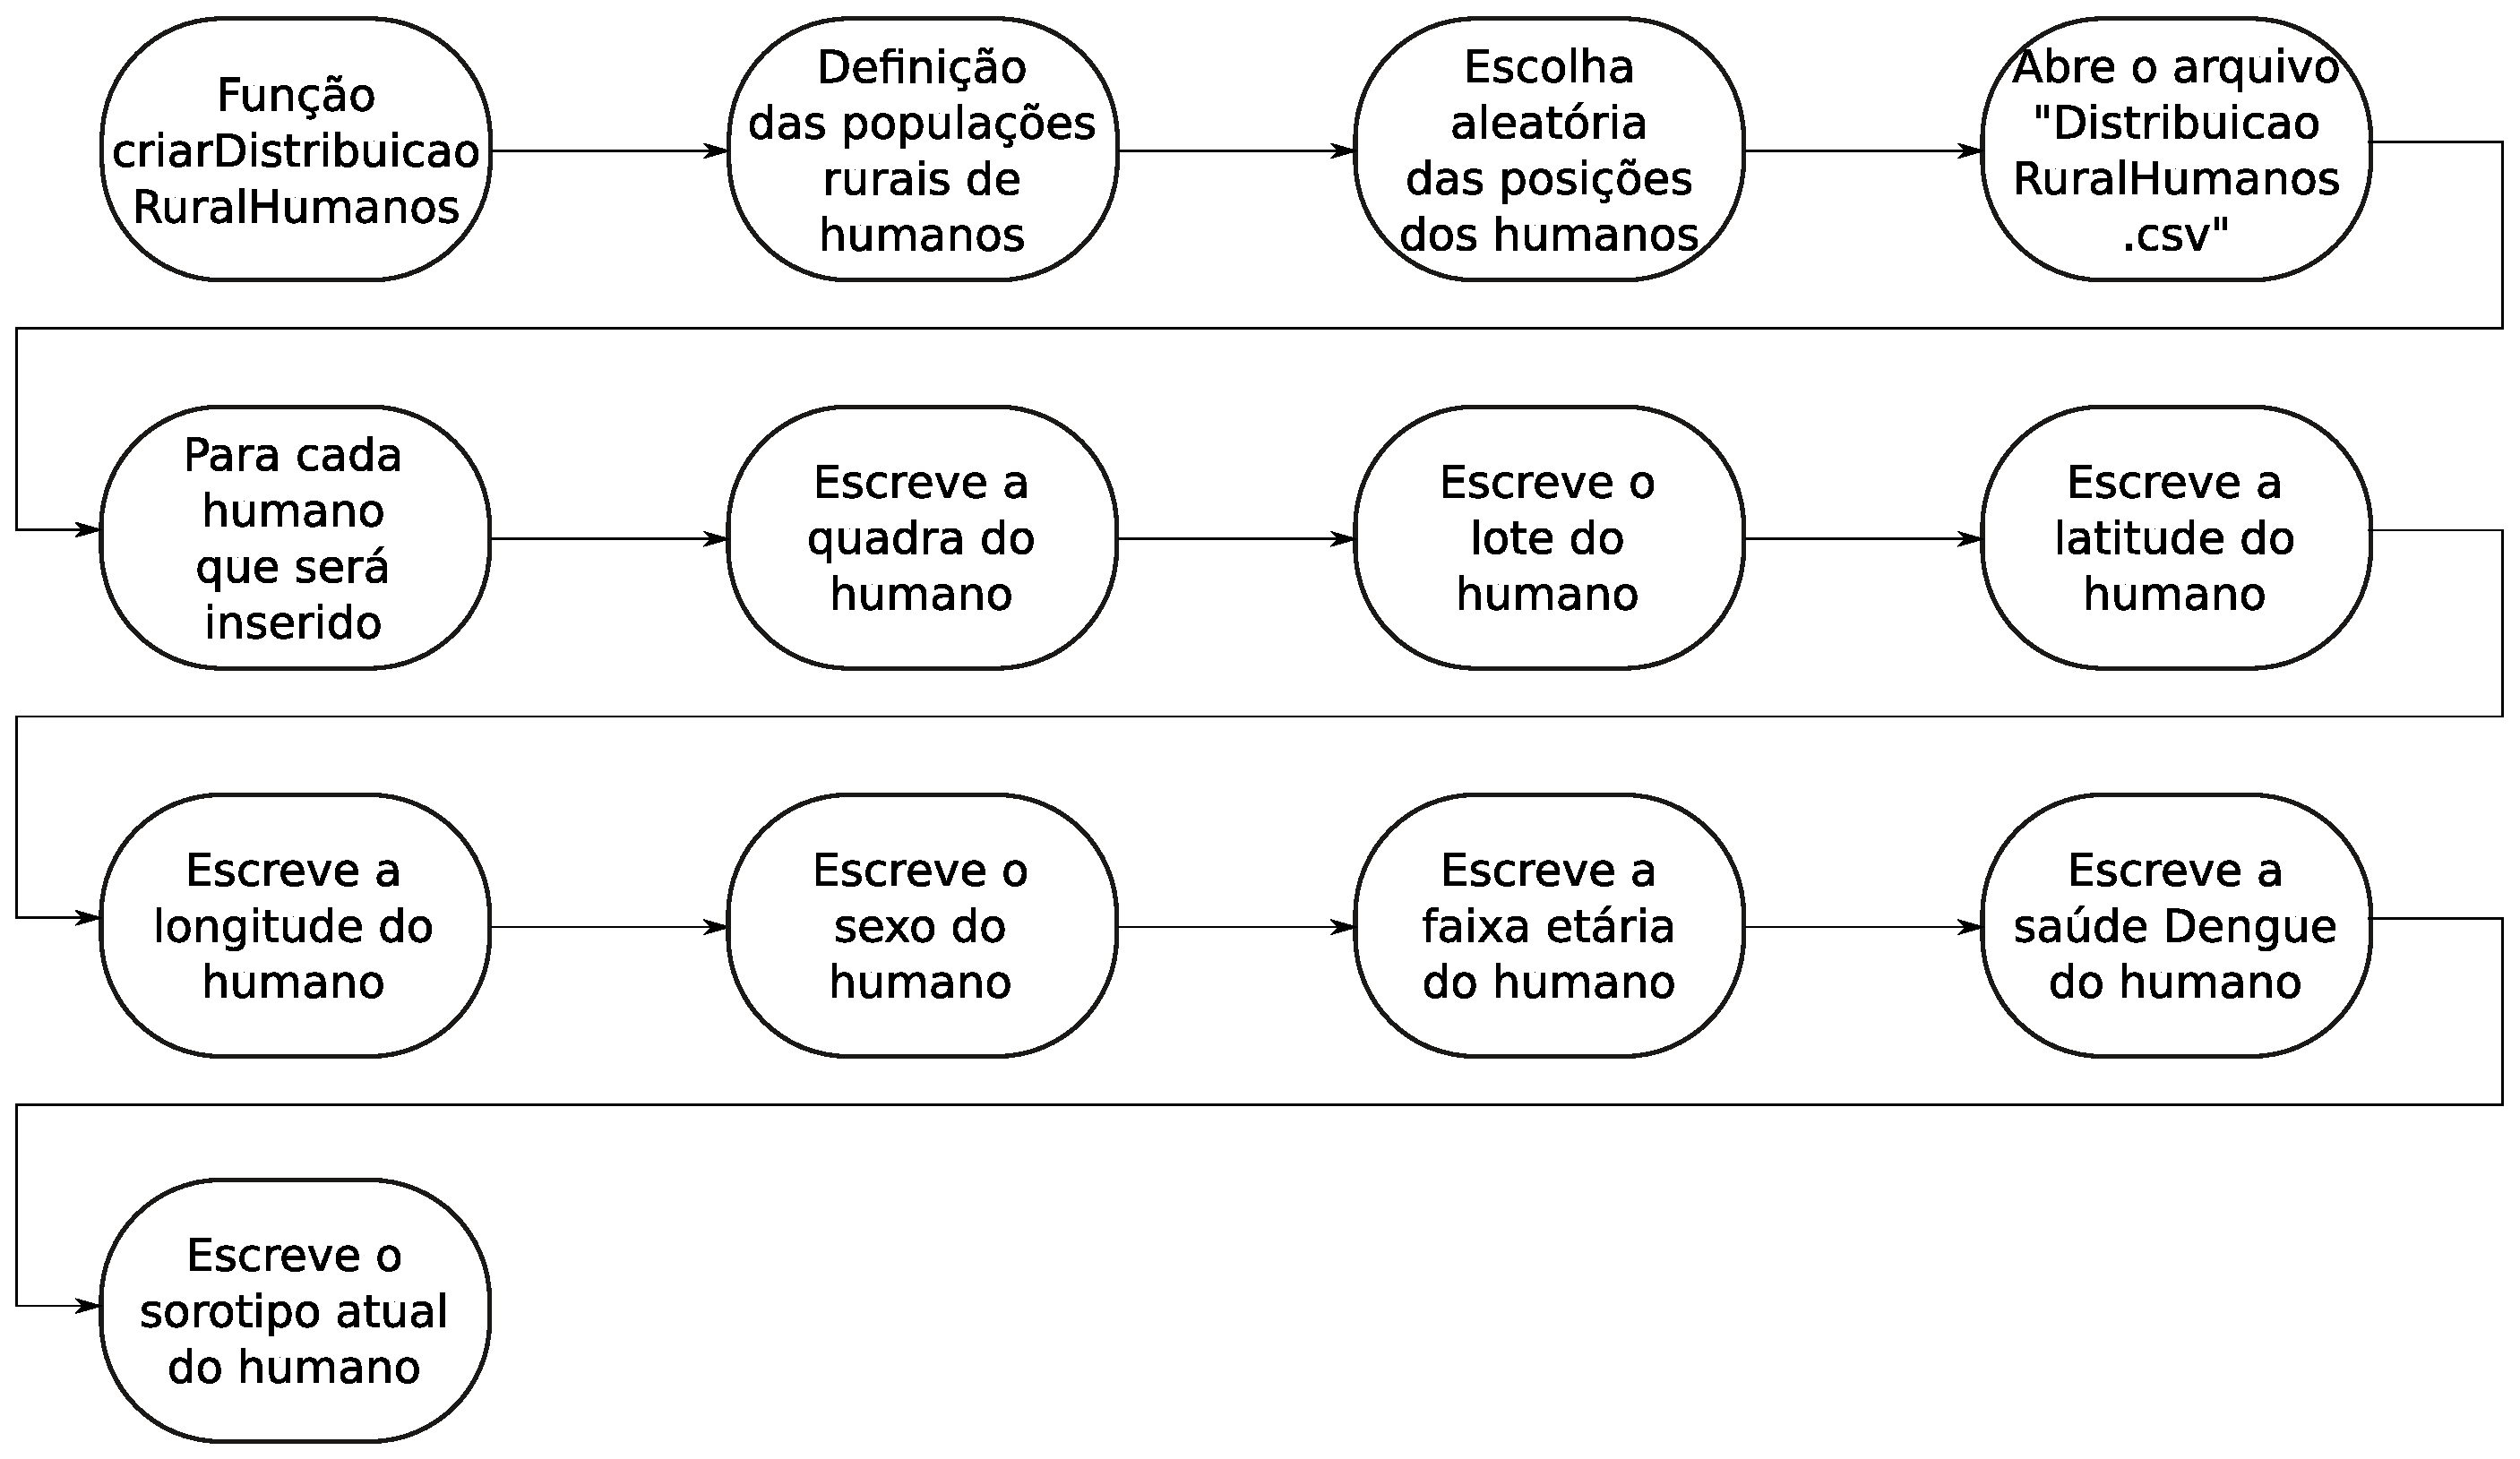
\includegraphics[width=0.8\textwidth]{Figuras/Simula/Fluxos/criarDistribuicaoHumanos.eps}
  \caption{Função criarDistribuicaoHumanos.}
  \label{fig:criarDistribuicaoHumanos}
\end{figure} 

\newpage

\subsubsection{Função gerarArquivoRegioes}

O Código \ref{cod:gerarArquivoRegioes}, Algoritmo \ref{alg:gerarArquivoRegioes} e Figura \ref{fig:gerarArquivoRegioes} ilustram a rotina responsável pela geração do arquivo que descreve as distintas regiões utilizadas na aplicação da vacinação e dos diferentes tipos de controle populacional e ambiental. Estas regiões são utilizadas em diversas operações durante a execução de simulações, destacando-se as rotinas de movimentação e gestação de agentes e controles populacionais e ambientais aplicadas sobre a população de agentes. 

\lstinputlisting[caption=Função gerarArquivoRegioes, label=cod:gerarArquivoRegioes, captionpos=b, language=Java]{Codigos/Simula/Fontes/gerarArquivoRegioes.java}

\begin{algorithm}[H]
   \SetAlgoLined   
   \input{Codigos/Simula/Algoritmos/gerarArquivoRegioes.txt}
   \caption{\textsc{Função gerarArquivoRegioes.}}
   \label{alg:gerarArquivoRegioes}
\end{algorithm}

\begin{figure}[H]
  \centering
  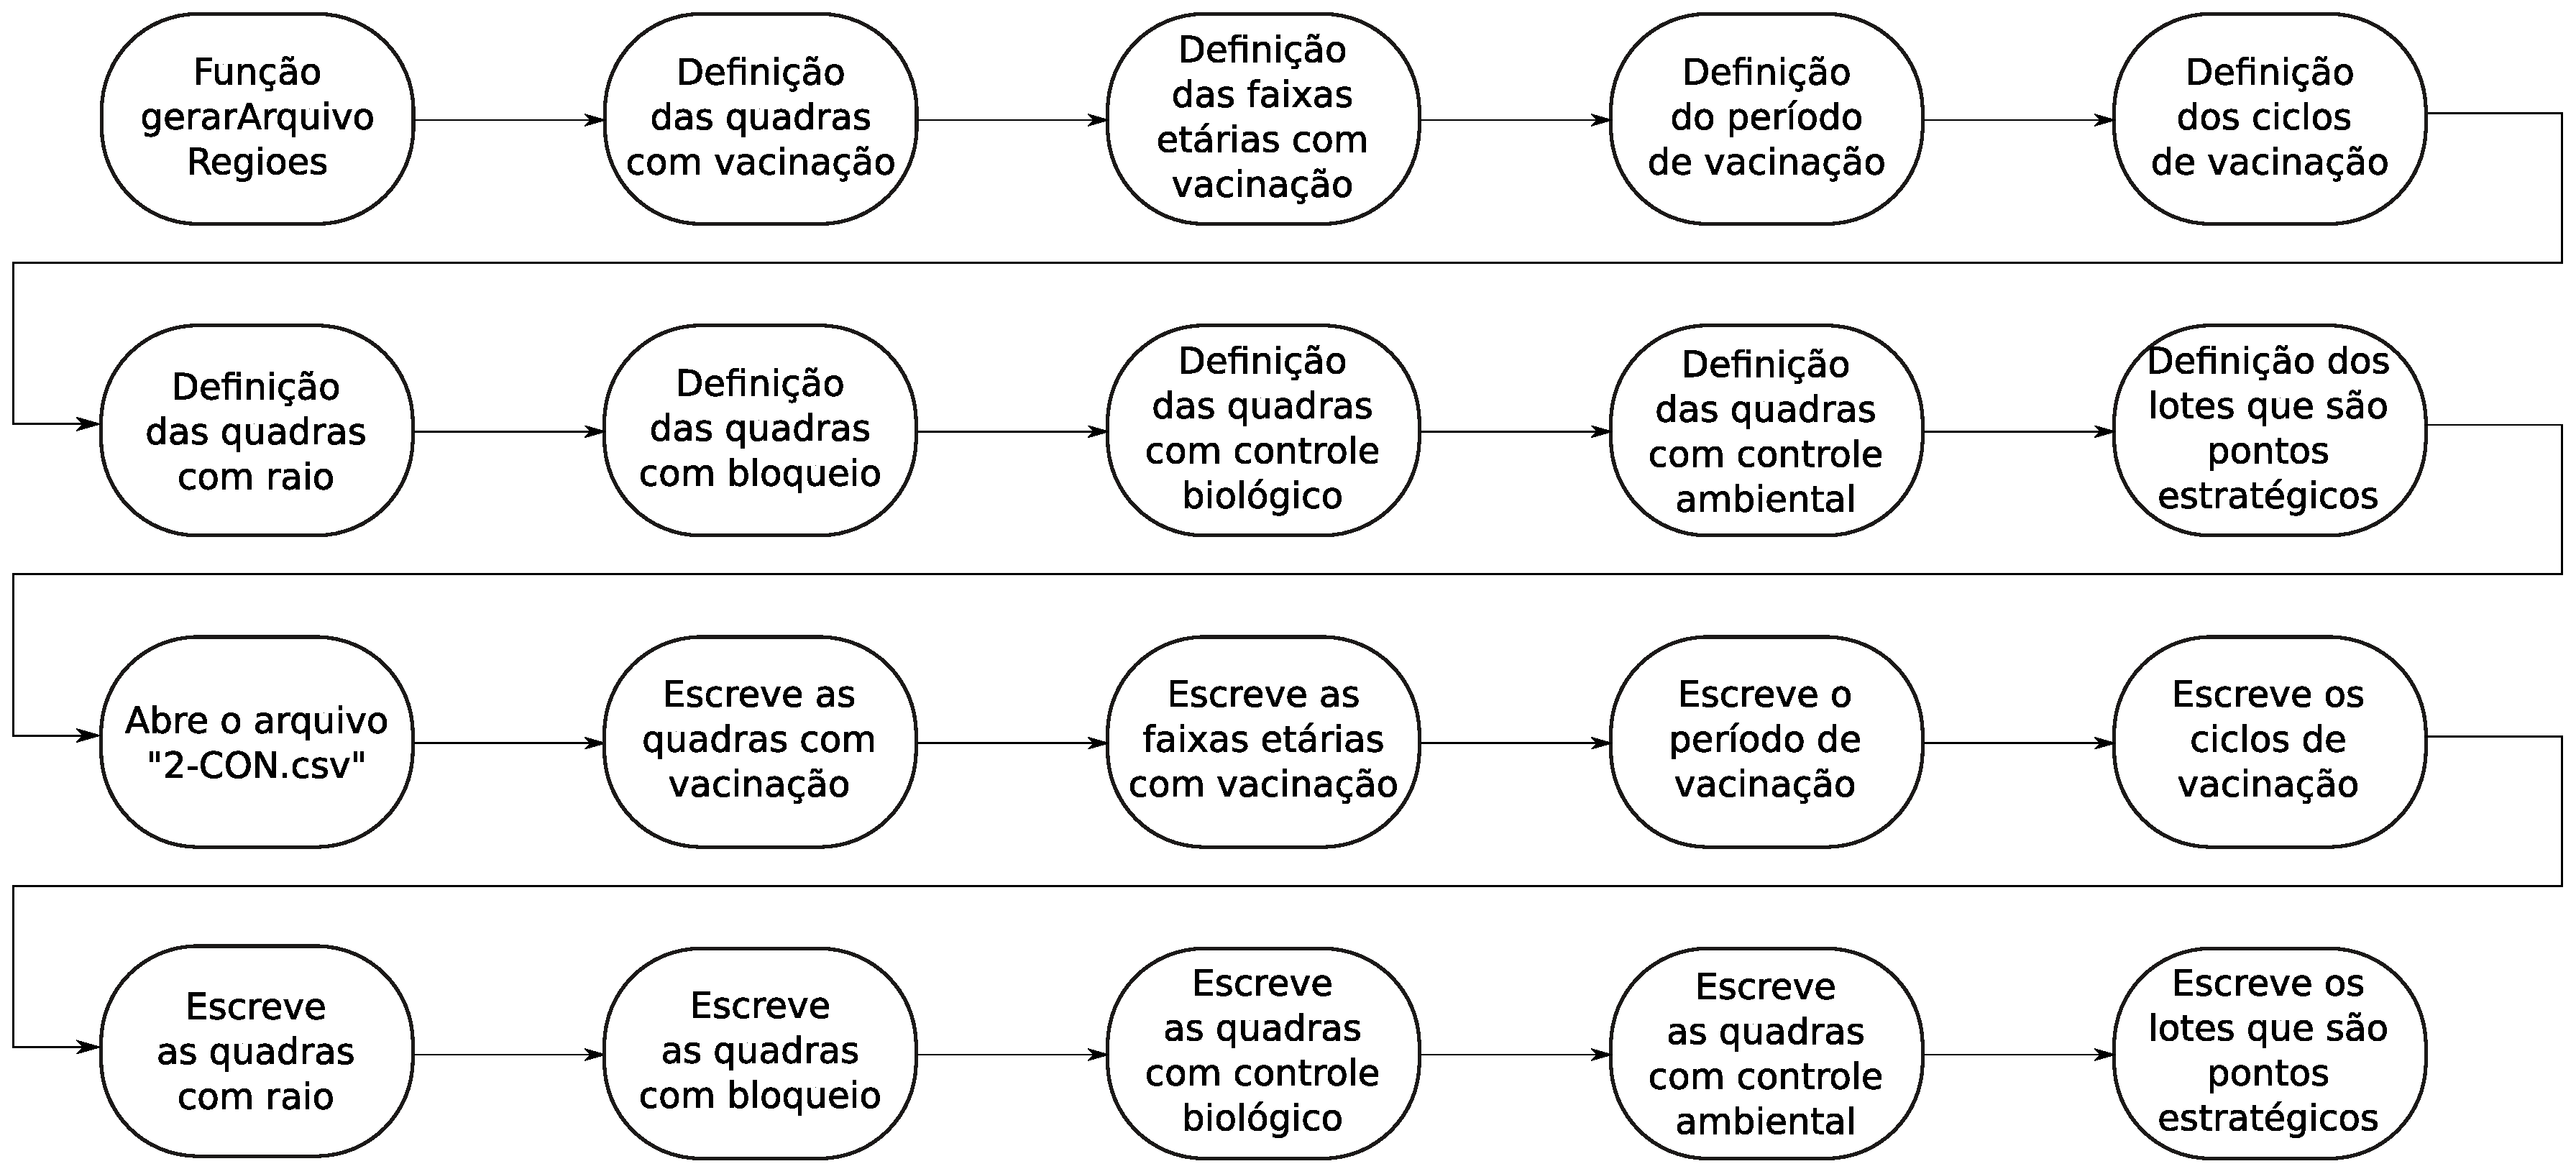
\includegraphics[width=1\textwidth]{Figuras/Simula/Fluxos/gerarArquivoRegioes.eps}
  \caption{Função gerarArquivoRegioes.}
  \label{fig:gerarArquivoRegioes}
\end{figure} 

\newpage
